% Document class with options: openright - chapters start on right-hand pages, twoside - two-sided layout, british - using British English language settings.
\documentclass[openright,a5paper,twoside]{book}

% Load the ptmt package, presumably for formatting.

\usepackage{ptmt}

% Load the blindtext package, which provides commands for generating dummy text.
\usepackage{blindtext}

% Set the title of the book.
\title{Сборник задач по строению вещества}

% Set the authors of the book (multiple authors separated by \and).
\author{First Author \and Second Author}

\setmainfont{Noto Serif}
\setsansfont{Noto Sans}
\setmonofont{Noto Sans Mono}


% Set the date to the current date.
%\date{\today}

% Begin the document.
\begin{document}

% Front matter section.
\frontmatter
% Include the title page, which is located in the FrontMatter subfolder.
% This code snippet creates a title page for a book.

%\setmainfont{Noto Sans}
%\setsansfont{Noto Sans}
%\setmonofont{Noto Sans Mono}

% The 'titlepage' environment starts the title page.
\begin{titlepage}
    \centering
    \small НОВОСИБИРСКИЙ ГОСУДАРСТВЕННЫЙ УНИВЕРСТИТЕТ\\
    КАФЕДРА ФИЗИЧЕСКОЙ ХИМИИ\\
    \vspace{14px}
    % The 'colorbox' is used to create a colored background for the book title and subtitle.
    % 'black!5' sets the color to 5% black (a light gray shade).
    \colorbox{white}{
        % The first 'parbox' is used to center the title and subtitle within the colored background.
        \parbox[t]{0.975\textwidth}{%
            % The second 'parbox' is used to center the title and subtitle text.
            \parbox[t]{0.95\textwidth}{%
                % Right-align the title and subtitle text, and set it in uppercase and huge font size.
                \centering\vspace{0.75cm}\huge\scshape
		%\setmainfont{Noto Sans}
                \textbf{СБОРНИК ЗАДАЧ\\ПО СТРОЕНИЮ ВЕЩЕСТВА} \\[3.5pt]
		%\setmainfont{Noto Serif}
                \large\bf
               % \vspace{0.5cm}
            }
        }
    }
    
    \vspace{16px}
    \centering \normalsize Мельников А.Р., Матвеева А.Г., Афимченко Н.А., Бакаев И.В., Алексеев В.А., Кравец Н.В., Михейлис А.В.
    % Vertically space the content evenly, pushing the text to the center of the page.
    \vspace{18px}
	\begin{figure}[h]
	    \centering
	    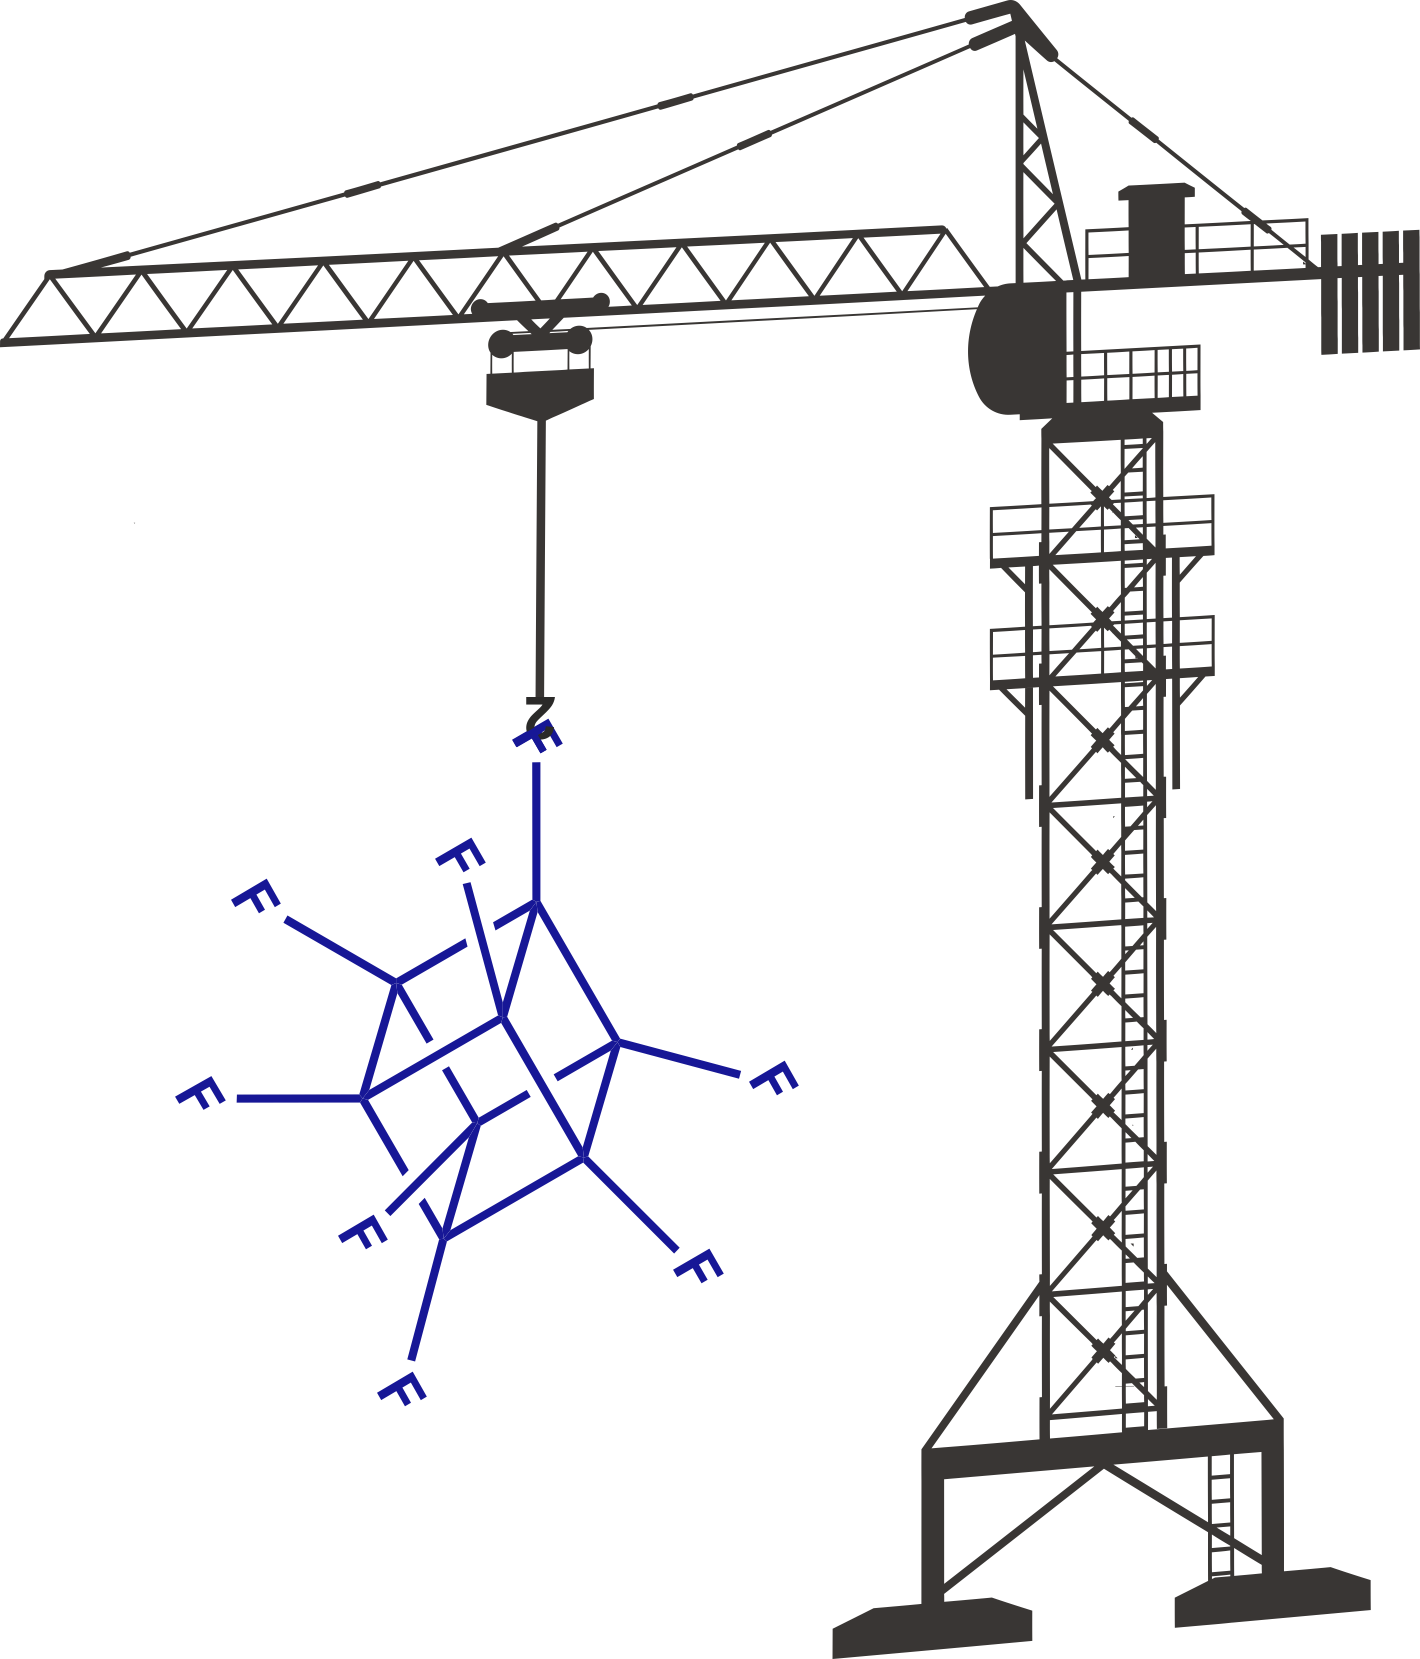
\includegraphics[width=0.73\textwidth]{images/title.png}
	\end{figure}

	%\vfill

    %, Ничипоренко В.А.
    % The first 'parbox' is used to display horizontal rules on both sides of the authors' information.
   % \parbox[t]{0.95\textwidth}{%
        % Right-align the horizontal rule and add some vertical space above and below it.
        %\hfill\rule{0.15\linewidth}{0.5pt}\\[7.5pt]
        % Right-align the authors' names and affiliations.
   %     \centering
        %\:{Мельников Анатолий\textsuperscript{\textdagger}\\
        %    Second Author\textsuperscript{\textdagger}}\\[4pt]
        
        % Display the superscript \textdagger symbol and authors' affiliations.
        %\normalsize} 
        %\\
        %\normalsize
        %2025\\
        % Right-align the second horizontal rule.
        %\hfill\rule{0.15\linewidth}{0.5pt}
    %}
\end{titlepage}


% Create the book's title page.
%\maketitle\pagebreak

% Include the dedication page from the FrontMatter subfolder.
%\include{./FrontMatter/dedication}

% Include the epigraph page from the FrontMatter subfolder.
%% This code snippet creates a quote block attributed to an author.

% Vertically space the content evenly, pushing the quote to the center of the page.
\vspace*{\fill}

% Set the font size to \Large (large) and the text style to italics.
\Large\textit{Если закрыть глаза, становится темно}

% Add some vertical space after the quote.
\bigskip

% The author's name is right-aligned and set in sans-serif small caps.
\begin{flushright}
    \sffamily\scshape Стетхэм
\end{flushright}

% Set the font back to the default (normal font size and style).
\normalfont\normalsize

% Vertically space the content evenly again, pushing any remaining space to the bottom of the page.
\vspace*{\fill}


% Include the foreword page from the FrontMatter subfolder.
%\include{./FrontMatter/foreword}

% Include the preface page from the FrontMatter subfolder.
\setstretch{1.2}
\footnotesize

\chapter*{Предисловие}

Настоящий сборник задач представляет собой учебное пособие к годовому курсу ''Строение вещества'', преподаваемого на химическом отделении факультета естественных наук Новосибирского государственного университета. Сборник разбит на два блока, соответствующих осеннему и весеннему семестру. Каждый блок в свою очередь разбит на 9 тем, соответствующих программе курса. Всего в сборнике приведено 223 задачи. Задачи, рекомендованные для рассмотрения на семинарских занятиях, отмечены буквой \textbf{С}. Задачи, предлагаемые на контрольных работах или экзаменах после 2022 года, отмечены буквой \textbf{K}. Задачи, предлагаемые в качестве теоретических вопросов на экзаменах после 2022 года, отмечены буквой \textbf{Т}. В сборник также включен список теоретических вопросов, предлагаемых на экзамене. Вопросы для переэкзаменовки отмечены буквой \textbf{П}. Все задачи снабжены краткими ответами или указаниями о подхода к решению. 

О~возможных ошибках в ответе, опечатках в условии задачи или в справочных данных просьба сообщать по электронной почте: anatoly.melnikov@tomo.nsc.ru 

%\undersign
%\thispagestyle{empty}

% Include the acknowledgement page from the FrontMatter subfolder.
%\include{./FrontMatter/acknowledgement}

% Table of contents page.
\footnotesize
\tableofcontents

% Main matter section.
\mainmatter

% Part 1: Preliminaries.
\chapter[Описание электронного строения  атомов и молекул]{\texorpdfstring{Описание электронного строения\\атомов и молекул}{Описание электронного строения  атомов и молекул}}
\thispagestyle{empty}

% Include Chapter 1 from the MainMatter subfolder.

\setmainfont{Noto Serif}
\setsansfont{Noto Sans}
\setmonofont{Noto Sans Mono}
\setstretch{1.35}
\footnotesize

\section{Угловой момент, сложение моментов}

1. Найти среднее значение потенциальной энергии в $1s$ состоянии атома водорода. Как полученная величина соотносится с полной и кинетической энергией? 
\par
2. Определите разницу в энергиях $1s$ орбиталей атома водорода и дейтерия.
\par
3. Сверхтонкое взаимодействие между спином электрона и спином ядра задается гамильтонианом $\widehat H = a (\vec S, \vec I\,)$, где $a$ – константа сверхтонкого взаимодействия, $\vec S$ и $\vec I$ – векторы, составленные из операторов электронного и ядерного спина. Определите на сколько уровней расщепится основное состояние атома водорода при учете этого взаимодействия, а также в явном виде выпишите полные волновые функции получившихся состояний.
\par
4. К атому водорода внезапно прилетает протон и прилипает к ядру. Определите чему равна вероятность остаться в основном состоянии?
\par
5С. Постройте полярные диаграммы вещественных сферических гармоник $\textit{Y}_{00}$, $\textit{Y}_{1m}$, $\textit{Y}_{2m}$. Объясните физический смысл полученных картинок.
\par
6С. Определить число спиновых функций симметричных и антисимметричных относительно перестановок для системы, состоящей из двух слабовзаимодействующих частиц со спином $S$. Рассмотрите случаи целого и полуцелого $S$.\par
7С. Постройте связь волновых функций мультипликативного базиса и базиса полного момента для системы двух моментов $L_1 = L_2 = 1$. Какова вероятность обнаружить каждое из значений полного момента, если система находится в~состоянии $\psi = \ket{1\,0}\ket{1\,0}.$
\par
8С. Сколько различных полных моментов существует в системе двух слабовзаимодействующих моментов $L_1 > L_2$?
\par
9С. Система из $N$ электронов, где $N$ – четное число, имеет $K$ возможных значений полного спина. Установите связь между $N$ и $K$. Сколько раз в данной системе встретится $K = 0$? Что изменится, если $N$ будет нечетным числом?
\par
10. Постройте матрицу оператора понижения $\widehat{S}_{-}$ для частицы со спином 5/2.
\par
11. Записать оператор скалярного произведения спинов двух слабо взаимодействующих частиц со спинами $S_1$ и $S_2$. Чему равно среднее значение этого оператора в триплетном и синглетном состояниях системы из двух спинов 1/2?
\par
12C. Определите кратность вырождения электронных уровней в атоме водорода в состоянии $\ket{n\,l\,m} $.
\par
13К. Система из двух слабовзаимодействующих моментов $S_1$, $S_2$ находится в~состоянии с волновой функцией $\ket{S_1\,S_1-1}\ket{S_2\,S_2}$. Определите вероятности обнаружения различных значений полного момента $S$, а также среднее значение квадрата полного момента $\braket{S^2}$.
\par
14С. Для системы из трех слабовзаимодействующих частиц со спинами $S + n$, $S$~и~$S - n$ определите общее число возможных значений полного спина. Считайте для определенности, что $n > 0$, a $S \geq n$.
\par
15C. Система из $2N$ электронов находится в состоянии, описываемой волновой функцией: $\alpha_1\beta_2\beta_3 \ldots \beta_{2N}$. Определите вероятность различных значений полного спина $S$ в этом состоянии.
\par
16. Постройте связь волновых функций мультипликативного базиса и базиса полного момента для системы трех электронов.
\par
17С. Определите количество состояний с определенными проекциями полного момента для системы из $N$ электронов. Как изменится ответ, если рассмотреть систему частиц с моментом 1.
\par
18К. Запишите полные волновые функции системы, состоящей из двух слабовзаимодействующих частиц с координатными функциями $\phi_1$ и $\phi_2$, для случаев: (1) неразличимых частиц со спином 1/2, (2) различимых частиц со спином 1/2, (3) неразличимых частиц со спином 0. В какой ситуации в реальной системе возможна реализация случая (2)?
\par
19. Определите чему равны следующие матричные элементы: $\braket{\textit{Y}_{22}|\widehat L^4_+|\textit{Y}_{2-2}}$, $\braket{\textit{Y}_{21}|3\widehat L_{z}^2- \widehat L^2|\textit{Y}_{21}}$, $\braket{\textit{Y}_{21}\textit{Y}_{20}|3 \widehat L_{z_1}^2- \widehat L_1^2+3 \widehat L_{z_2}^2- \widehat L_2^2|\textit{Y}_{21}\textit{Y}_{20}}$.
\par
20C. Система из $N$ электронов находится в состоянии, описываемой волновой функцией $\psi=\alpha_1\alpha_2 \ldots \alpha_n\beta_{n+1}\beta_{n+2} \ldots \beta_{N}$. Определите среднее значение квадрата суммарного спина системы.
\par

\setmainfont{Noto Serif}
\setsansfont{Noto Sans}
\setmonofont{Noto Sans Mono}
\setstretch{1.35}
\hyphenation{ма-те-ма-ти-ка вос-ста-нав-ли-вать дан-ный}


\section{Термы многоэлектронного атома}

1С. Определите все термы и мультиплеты электронной конфигурации $p^3$ в~пределе слабого по сравнению с межэлектронным отталкиванием взаимодействием между спиновым и орбитальным моментом.
\par
2С. Определите основной терм и основной мультиплет для электронной конфигурации $6s^24f^3$ в пределе слабого по сравнению с межэлектронным отталкиванием спин-орбитального взаимодействия.
\par
3С. Определите все термы и мультиплеты электронной конфигурации $2p^23p^3$ в~пределе слабого по сравнению с межэлектронным отталкиванием спин-орби-тального взаимодействия.
\par
4С. Определите основной терм электронной конфигурации $l^n$ в пределе слабого по сравнению с межэлектронным отталкиванием спин-орбитального взаимодействия.
\par
5С. Для электронной конфигурации $l^{4l}$ в предельном случае слабого по сравнению с межэлектронным отталкиванием спин-орбитального взаимодействия определите основной терм, общее число термов, а также число термов определенной мультиплетности.
\par
6С. Постройте корреляционную диаграмму между предельными случаями слабого и сильного спин-орбитального взаимодействия для электронной конфигурации $p^5s^1$.
\par
7С. Определите, какому терму и какой электронной конфигурации атома принадлежит волновая функция, имеющая вид:
\begin{equation*}
\begin{aligned}
\psi &=\frac{1}{\sqrt{6}}[\sqrt{2}(\textit{Y}_{21}\textit{Y}_{11}-\textit{Y}_{11}\textit{Y}_{21})+(\textit{Y}_{22}\textit{Y}_{10}-\textit{Y}_{10}\textit{Y}_{22})]\cdot\xi_S, \hspace{28mm}
\end{aligned}
\end{equation*}
где $\xi_S$ представляет собой некоторую спиновую частью волновой функции.
\par
8С. Определите все термы электронной конфигурации $p^3$ в~пределе сильного, по сравнению с межэлектронным отталкиванием, спин-орбитального взаимодействия.
\par
9С. В пределе LS связи определите все термы электронной конфигурации $h^2$.
\par
10К.  Пять первых уровней основного терма атома железа $[\text{Ar}]3d^64s^2$ имеют следующие значения относительной энергии (см$^{-1}$): 0; 415,9; 704,0; 888,1; 978,1. Определите величину константы спин-орбитального взаимодействия.
\par
11. В пределе LS связи определите все функции основного терма электронной конфигурации $p^3$.
\par
12. Определите возможную электронную конфигурацию атома, если известно, что без учета спин-орбитального взаимодействия ее основной терм $^9G$.
\par
13. Определите чему равен параметр $m$, соответствующий максимальному вырождению основного терма электронной конфигурации $l^m$.
\par
14. В пределе LS связи определите количество термов с максимальным спином для электронной конфигурации $l^3$.
\par
15К. Определите основной терм конфигурации $s^1l^n$ в случае слабого спин-орби-тального взаимодействия.
\par
16С. Сколько различных состояний с определенным значением $J$ будет возникать из электронной конфигурации $l^2$ в случае слабого и сильного спин-орби-тального взаимодействия.
\par
17К. Покажите, что средняя энергия всех мультиплетов, возникающих из терма $^{2S+1}L$, равна энергии этого терма. Для определенности считайте, что $L\ge S$. Дополнительные справочные данные:
\begin{equation*}
\begin{aligned}
&\sum_{i=0}^{n} i = \frac{1}{2}n(n+1);\quad \sum_{i=0}^{n} i^{\,2} = \frac{1}{6}n(n+1)(2n+1);\quad \sum_{i=0}^{n} i^{\,3} = \frac{1}{4}n^2(n+1)^2;\hspace{11mm}
\\[6pt]
 &\sum_{i=k}^{n+k} i = \frac{1}{2}(2k+n)(n+1);\quad \sum_{i=k}^{n+k} i^{\,2} = \frac{1}{6}(n+1)(6k^2+n+6kn+2n^2);\,
 \\[6pt]
&\sum_{i=k}^{n+k} i^{\,3} = \frac{1}{4}(n+1)(2k+n)(2k^2+n+2kn+n^2).
\end{aligned}
\end{equation*}
\par
18К. Между предельными случаями LS и jj связей возможны различные промежуточные случаи, которые реализуются в основном для электронных конфигураций, возникающих при возбуждении одного электрона из замкнутой электронной оболочки. Одним из таких примеров является JK связь. В этом случае обозначение термов имеет вид: $^{2s_2+1}[K]_J$ , где $\vec{l}_1+\vec{s}_1=\vec{j}_1$, $\vec{j}_1+\vec{l}_2=\vec{K}$, $\vec{K}+\vec{s}_2=\vec{J}$, a $\vec{s}_2$, $\vec{l}_2$ – моменты внешнего электрона, возбуждаемого из замкнутой оболочки. Определите все термы иона $\text{Kr}^{+26}$ в первом возбужденном состоянии c электронной конфигурацией $[$Be$]2p^5 3d^1$.
\par
19. Найти нормировочный множитель $A$ для радиальных слейтеровских функций $R_n(r)=A\left( \sfrac{r}{a_0} \right) ^{n^*-1}\exp[-\xi r/ a_0]$, где $n^*$ – эффективное главное квантовое число, $\xi=\frac{Z-s}{n^*}$, $Z$ – заряд ядра, $s$ – константа экранирования, $a_0$ – радиус Бора. Найти радиус, при котором плотность вероятности данных функций максимальна. Пользуясь полученным выражением, оценить размер атома железа.
\par

\setmainfont{Noto Serif}
\setsansfont{Noto Sans}
\setmonofont{Noto Sans Mono}
\setstretch{1.35}
\hyphenation{ма-те-ма-ти-ка вос-ста-нав-ли-вать}


\section{Дипольные переходы между термами}

1К. Рассчитайте величину электрического дипольного момента перехода между атомными орбиталями $2s$ и~$2p_z$ в~атоме водорода.
\par
2К. Возбужденное состояние атома кальция имеет электронную конфигурацию $1s^22s^22p^63s^23p^63d^14f^1$. Определите все мультиплеты этой конфигурации. Укажите какой из мультиплетов является основным. Атом кальция находится в~состоянии $^3F_2$, порождаемом некоторой другой возбужденной конфигурацией. В какие мультиплеты из найденных разрешен электрический дипольный переход? Какой четностью должна обладать данная возбужденная конфигурация?
\par
3К. Для электронной конфигурации $6s^2 4f^4$ определите: (1) полное количество термов, (2) основной терм, считая спин-орбитальное взаимодействие слабым, (3) одну возбужденную конфигурацию, в которую возможен электрический дипольный переход из исходной электронной конфигурации.
\par
4К. В атоме углерода исследуют электрические дипольные переходы между следующими электронными конфигурациями:
\begin{equation*}
\begin{aligned}
\relax [\text{He}]2s^2 2p^2 \rightarrow \{[\text{He}]2s^1 2p^2 3s^1, [\text{He}]2s^1 2p^2 3p^1, [\text{He}]2s^2 2p^1 3p^1\}.\hspace{19mm}
\end{aligned}
\end{equation*}
Пренебрегая спин-орбитальным взаимодействием, определите сколько всего возможно переходов между данными конфигурациями. При учете спин-орбитального взаимодействия тонкая структура одного из переходов между триплетными термами состоит из 5 линий. Определите каким именно термам соответствует этот переход. Эффективная константа спин-орбитального взаимодействия одинакова во всех термах.
\par
5К. В спектре поглощения атома кальция среди прочих наблюдаются три серии линий, обозначенных A, B, C и соответствующих длинам волн (нм): A:~\{428,30; 428,94; 429,90; 430,25; 430,77; 431,87\}, B: \{394,89; 395,71; 397,37\}, C: \{585,74; 551,30\}. Какие из указанных серий относятся к переходам между мультиплетами электронных конфигураций (1): $[\text{Ar}]4s^14p^1 \rightarrow [\text{Ar}]4p^2$, а какие к переходам между мультиплетами электронных конфигураций (2): $[\text{Ar}]4s^14p^1$ $\rightarrow$ $[\text{Ar}]4p^16s^1$.
\par
\setmainfont{Noto Serif}
\setsansfont{Noto Sans}
\setmonofont{Noto Sans Mono}
\setstretch{1.35}
\hyphenation{ма-те-ма-ти-ка вос-ста-нав-ли-вать}


\section{Многоэлектронный атом во внешних полях}

1С. Определите расщепление самой длинноволновой линии поглощения иона $\text{Ti}^{3+}$ в слабом магнитном поле. Рассмотрите случаи комнатной температуры и~температуры, близкой к абсолютному нулю.
\par
2С. Найти один мультиплет, $g$-фактор которого равен $-10$.
\par
3. Определить на сколько линий расщепляется спектральная линия, соответствующая переходу $^{2S+1}L_J$ $\rightarrow$ $^{2S+1}[L-1]_{J-1}$, в слабом магнитном поле при использовании неполяризованного света.
\par
4К. Тонкая структура линии, соответствующей в некотором атоме электронному переходу между термами $^3P \,\rightarrow\,^3D$, в сильном магнитном поле имеет вид~(см$^{-1}$): 21977,9; 21978,02; 21978,14; 21978,96; 21979,78; 21979,9; 21980,02. Определите эффективную константу спин-орбитального взаимодействия, считая, что она в указанных термах одинакова. Чему равна индукция магнитного поля, в котором был зарегистрирован описанный спектр? Магнетон бора равен 14~ГГц$\cdot$Тл$^{-1}$, скорость света равна 3$\cdot$10$^8$ м$\cdot$с$^{-1}$.
\par
5С. Найти расщепление самой длинноволновой линии атома бора в сильном магнитном поле.
\par
6С. На сколько уровней с различной энергией расщепляется основной терм атома с электронной конфигурации $l^l$ в сильном магнитном поле? Какое максимальное вырождение соответствует этим уровням и сколько будет уровней с найденным максимальным вырождением?
\par
7. Для возбужденного состояния атома водорода с $n = 2$ реализуются мультиплеты $^2S_{1/2}$, $^2P_{1/2}$, $^2P_{3/2}$. Первые два мультиплета имеют одинаковую энергию. Каким образом расщепятся мультиплеты $^2S_{1/2}$, $^2P_{1/2}$ при включении постоянного электрического поля напряженностью $E$.
\par
8. Спиновая мультиплетность основного терма электронной конфигурации, заполненной более чем наполовину, равна $S$. В этом состоянии имеется $k$ пар спаренных электронов. Определите $g$-фактор наименьшего по энергии мультиплета, возникающего из этого терма.
\par
9. Определить число линий и расстояние между ними при расщеплении в~слабом магнитном поле второй линии серии Бальмера атома водорода при поляризации, совпадающей с направлением внешнего магнитного поля.
\par
10. Определить количество уровней с различной энергией, на которое расщепится уровень атома водорода с главным квантовым числом $n = 100$ в~постоянном электрическом поле напряженностью $E$.
\par
11С. Определить расщепление электронной конфигурации $p^2$ в очень сильном магнитном поле, энергия взаимодействия с которым больше, чем энергия межэлектронного отталкивания, но меньше, чем энергия кулоновского взаимодействия электронов с ядром.
\par
12. Определите $g$-фактор основного терма электронной конфигурации $2s^12p^1$ в~случае jj связи.
\par
13С. Качественно нарисовать спектр поглощения атома водорода, помещенного во внешнее электрическое поле напряженностью $E$, в районе второй линии Лаймана. Указать поляризацию компонент спектра.
\par
14К. Основной терм электронной конфигурации $l^4$ вырожден 65 раз. Определите, что это за терм и чему равен $l$, считая спин-орбитальное взаимодействие слабым. На сколько уровней и с каким расстоянием между ними расщепится основной мультиплет найденного терма в слабом, по сравнению со спин-ор-битальным взаимодействием, магнитном поле?
\par
15. Рассчитайте $g$-факторы мультиплетов с наименьшей и наибольшей энергией, возникающих из основного терма электронной конфигурации $[2k]^{4k}$, где $k>0$ в пределе слабого по сравнению с межэлектронным отталкиванием взаимодействием между спиновым и орбитальным моментом.
\par

\setmainfont{Noto Serif}
\setsansfont{Noto Sans}
\setmonofont{Noto Sans Mono}
\setstretch{1.35}
\hyphenation{ма-те-ма-ти-ка вос-ста-нав-ли-вать}


\section{Правила Вигнера-Витмера}
1С. Чему равно число независимых волновых функций, которые соответствуют молекулярным термам $^1\Sigma^-$, $^3\Sigma^+$, $^3\Pi$, $^1\Phi$, $^6\Delta$?
\par
2С. Какие молекулярные термы возникают при сближении атомов углерода в~состоянии $^3P_g$ и азота в состоянии $^4S_u$?
\par
3С. Определите термы молекулы фтора, которые могут возникнуть при ее образовании в результате сведения: (1) двух атомов фтора в основном состоянии, (2)~двух атомов фтора, один из которых имеет однократно возбужденную $(s \rightarrow p)$ электронную конфигурацию, (3) ионов $\text{F}^+$ и $\text{F}^-$ в основных состояниях.
\par
4С. Определите полное количество термов, которые могут возникнуть при образовании гетероядерной молекулы из двух атомов, находящихся в состояниях $^{2S_1 + 1}L_1$ и $^{2S_2 + 1}L_2$. Для определенности считайте, что $L_1 \geq L_2$ и $S_1 \geq S_2$.
\par
\begin{wrapfigure}{r}{35mm} %this figure will be at the right
    \centering
    \vspace{0mm}
    
\includegraphics[width=35mm]{images/Fig_1_5_5.png}
    \vspace{-5mm}
\end{wrapfigure}
5. Определите электронные термы, которые могут возникнуть при сближении двух атомов водорода и~двух атомов дейтерия, как это показано на рисунке, с образованием линейной молекулы $\text{H}_2 \text{D}_2$.
\par
6К. Определите термы молекулы, образующейся при сведении атомов бериллия и кислорода в основных состояниях. Может ли при этом получиться основное состояние молекулы $\text{BeO}$? Если нет, то предложите возможное возбужденное состояние одного из атомов в паре (соответствующий терм атома и~электронная конфигурация), при котором возможно образование молекулы в~основном состоянии.
\par
7К. В газовой фазе при низких температурах исследовался распад молекулы $\text{BeF}$, находящейся в электронном состоянии $^1 \Sigma ^-$ . Можно ли однозначно сказать по гетеролитическому ($\text{Be}^+$, $\text{F}^-$) или гомолитическому ($\text{Be}$, $\text{F}$) механизму идет данная реакция, если в результате проведенных экспериментов были зарегистрированы продукты распада $\text{BeF}$ только в своих основных электронных состояниях?
\par
8. Может ли при сведении атомов $\text{C}$ ($2s^2 2p^2$) и $\text{O}$ ($2s^2 2p^4$) в основных состояниях получиться молекула $\text{CO}$ в основном состоянии?
\par
9. Определить молекулярные термы, которые могут возникнуть при сближении двух атомов гелия, находящихся в нижнем по энергии возбужденном состоянии, полученным из основного под действием электромагнитного излучения.
\par
10. Определите полное количество четных термов, которые могут возникнуть при образовании гетероядерной молекулы из двух атомов, находящихся в~одинаковых состояниях $^{2S + 1}L$.
\par
\setmainfont{Noto Serif}
\setsansfont{Noto Sans}
\setmonofont{Noto Sans Mono}
\setstretch{1.35}
\hyphenation{ма-те-ма-ти-ка вос-ста-нав-ли-вать}


\section{Электронное строение двухатомных молекул}

1С. С помощью теории МО ЛКАО рассмотреть электронное строение молекулы фтора. Определите основной терм, а также термы катион-, анион-радикала молекулы фтора и термы первого возбужденного состояния. Укажите также несколько разрешенных электрических дипольных переходов в данной молекуле.
\par
2. Проверьте, что дипольный момент молекулы водорода в основном и возбужденном состоянии равен нулю, в то время как дипольный момент одноэлектронного перехода отличен от нуля.
\par
3С. Молекула угарного газа является хорошим лигандом в координационной химии. Используя теорию МО ЛКАО объясните с чем это связано. Каким атомом координируется угарный газ в комплексах? Как это можно объяснить исходя из его электронного строения? Энергия атомных орбиталей углерода равна $E_{2s}$ = $-$19,4 эВ, $E_{2p}$ = $-$10,7 эВ. Энергия атомных орбиталей кислорода равна $E_{2s}$~= $-$32,4 эВ, $E_{2p}$ = $-$15,9 эВ. Точный расчет (RHF/3-21G*) показывает, что вклад различных атомных орбиталей в третью по энергии $\sigma$ молекулярную орбиталь равен, соответственно, $\text{C}_{2p_z}$ $\approx$ 32\%, $\text{C}_{2s}$ $\approx$ 56\%, $\text{O}_{2p_z}$ $\approx$ 11\%.
\par
4С. С помощью теории МО ЛКАО показать, что  $\text{He}_2$ является неустойчивой молекулой, а $\text{He}_2^{+}$ – устойчивой. Определите порядок связи в указанных двух молекулах.
\par
5. Определите основной терм $\text{OH}^-$ и $\text{OH}$.
\par
6К. Определите основной терм молекулы $\text{NO}$. В результате значительного спин-орбитального взаимодействия $\text{NO}$ при низкой температуре практически не~проявляет магнитных свойств. Объясните этот факт, считая, что при учете спин-орбитального взаимодействия состояния молекулы $^{2S+1}\Lambda$ расщепляются по величине полной проекции на ось молекулы $\Omega = \Lambda + M_s$, которая пробегает ряд значений от $\Lambda + S$ до $\Lambda - S$ через единицу. Почему магнитные свойства появляются при повышении температуры?
\par
7. Найти основной терм молекулы $\text{MoC}$. Можно ли получить основное электронное состояние $\text{MoC}$ при сведении атомов $\text{Mo}$ и $\text{C}$ в основных состояниях. Энергия атомных орбиталей углерода равна $E_{2s}$ = $-$19,4 эВ, $E_{2p}$ = $-$10,7 эВ. Энергия атомных орбиталей молибдена равна $E_{5s}$ = $-$7,4 эВ, $E_{5d}$ = $-$9,1 эВ.
\par
8. Найти основной терм линейной молекулы $\text{C}_3$. Что изменится при замене одного или двух атомов углерода на азот? Рассмотреть все возможные варианты замены атомов углерода. 
\par
\setmainfont{Noto Serif}
\setsansfont{Noto Sans}
\setmonofont{Noto Sans Mono}
\setstretch{1.35}
\hyphenation{ма-те-ма-ти-ка вос-ста-нав-ли-вать}
\input{insbox}

\section{Электронное строение многоатомных молекул}
1К. Определите поляризацию самой длинноволновой линии поглощения линейного катион-радикала $\text{BeH}_2^{+\boldsymbol{\cdot}}$. Потенциал ионизации $1s$ электрона водорода равен 13,6 эВ, $2s$ электрона атома бериллия 9,3 эВ. Разница между $2s$ и $2p$ подуровнями в атоме бериллия равна 3,4 эВ.
\par
%\vspace{\parskip}
%\InsertBoxR{0}{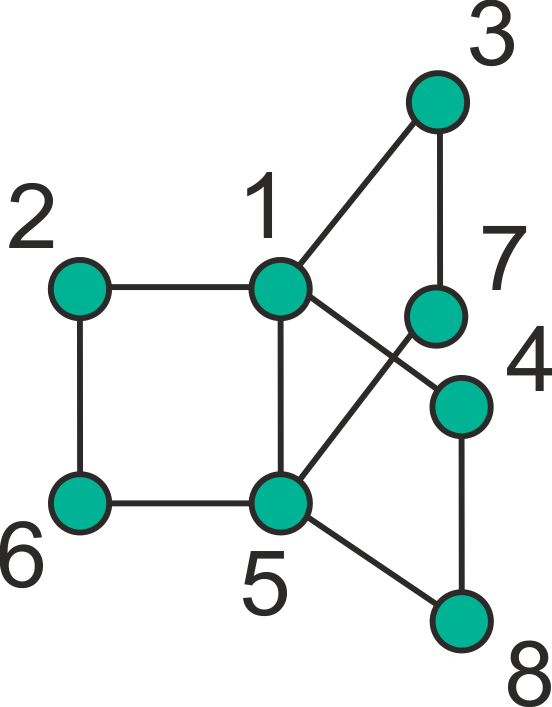
\includegraphics[width=10mm,height=10mm,keepaspectratio]{images/Fig_1_7_1.png}}[0]
\begin{wrapfigure}{r}{20mm} %this figure will be at the right
    \centering
    \vspace{-5.6ex}
     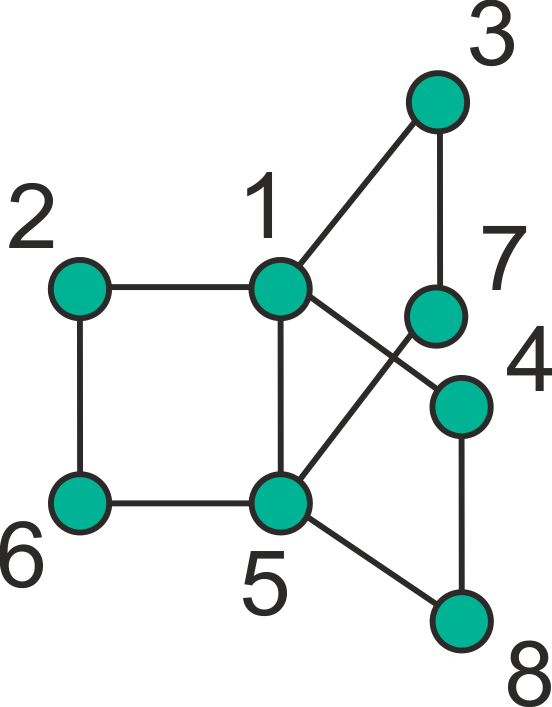
\includegraphics[width=14mm]{images/Fig_1_7_1.png}
    \vspace{-6mm}
\end{wrapfigure}
%\vspace{0.5pc}
2С. В базисе $1s$ орбиталей определите электронное строение хюккелевской системы, строение которой приведено на рисунке справа. Определите основной терм, а также количество разрешенных электрических дипольных переходов.
\par
3С. С помощью теории МО ЛКАО рассмотрите электронное строение молекулы озона, считая ее линейной. Определите основной терм.
\par
%\vspace{\parskip}
%\InsertBoxR{0}{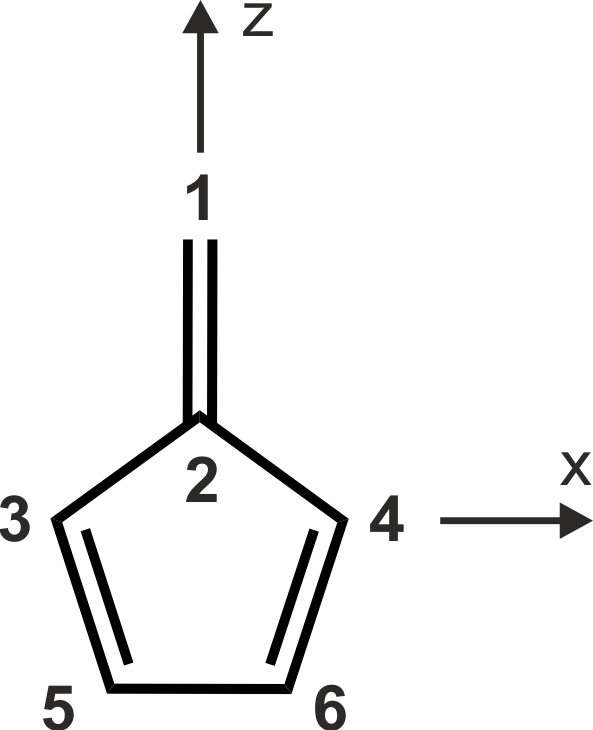
\includegraphics[width=10mm,height=10mm,keepaspectratio]{images/Fig_1_7_2.png}}[3]
\begin{wrapfigure}{r}{20mm} %this figure will be at the right
    \centering
    \vspace{-8.5mm}
    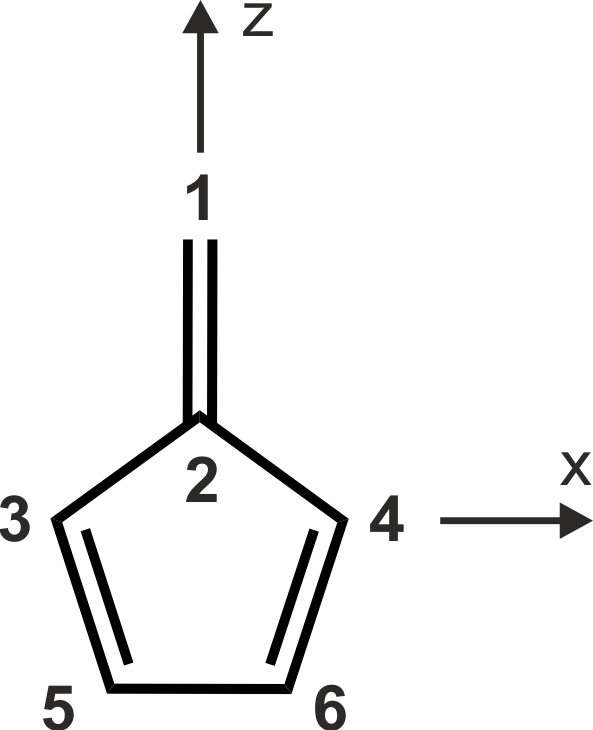
\includegraphics[width=17mm]{images/Fig_1_7_2.png}
    \vspace{-5mm}
\end{wrapfigure}
4К. Определите энергетические уровни $\pi$-системы изомера бензола – фульвена, структурная формула которого приведена на~рисунке. Чем может быть вызвано наличие большого дипольного момента у данной молекулы?
\par
5К. Используя теорию МО ЛКАО качественно определите электронное строение молекулы метана. Определите терм основного состояния нейтральной молекулы и ее катион- и анион-радикалов. Какой из указанных ионов/молекулы обладает наибольшей устойчивостью?
\par
\begin{wrapfigure}{r}{20mm} %this figure will be at the right
    \centering
    \vspace{0mm}
    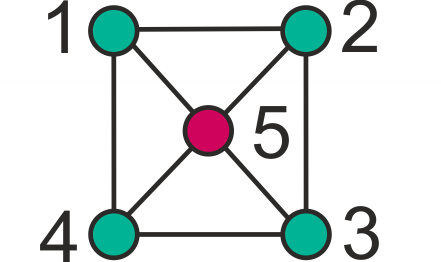
\includegraphics[width=17mm]{images/Fig_1_7_6.png}
    \vspace{-3.6mm}
\end{wrapfigure}
6С. Определите спиновую плотность хюккелевской системы, строение которой приведено на рисунке справа, в базисе $2p_z$ орбиталей. Как изменится полная электронная энергия данной системы при замене центрального атома, с кулоновским интегралом равным $\alpha$, на другой атом, с кулоновским интегралом равным $1,1\alpha$. Считайте, что резонансные интегралы при этом не изменились.
\par
7К. Постройте корреляционную диаграмму трех первых синглетных термов молекулы воды при изменении угла $\text{H}-\text{O}-\text{H}$ от 110º до 180º. Относительные энергии термов равны, соответственно, $^1A_1$, $^1B_1$, $^1A_2$: 0,0 эВ, 7,2 эВ, 8,0 эВ и $^1\Sigma _g^+$, $^1\Pi _u$, $^1\Pi _g$: 2,0 эВ, 6,4 эВ, 11,2 эВ. Каким электронным конфигурациям соответствуют указанные термы? Энергии атомных орбиталей кислорода и водорода равны: $E(2s,\text{O})$ = $-$32,4 эВ, $E(2p,\text{O})$ = $-$15,9 эВ, $E(1s,\text{H})$ = $-$13,6 эВ. При рассмотрении нелинейной молекулы воды считайте, что ось $x$ перпендикулярна плоскости молекулы.
\par
8К. Определите энергетические уровни и полную электронную энергию $\pi$-сис-темы аллильного радикала учитывая перекрывание $p_z$ орбиталей, которое задается интегралом перекрывания $S$. Считайте, что $S$ равен 0,25 для $p_z$ орбиталей соседних центров и равен 0 в ином случае. Сравните результат со~стандартным методом Хюккеля.
\par
9. Определите электронное строение ферроцена.
\par
\begin{wrapfigure}{r}{20mm} %this figure will be at the right
    \centering
    \vspace{0mm}
    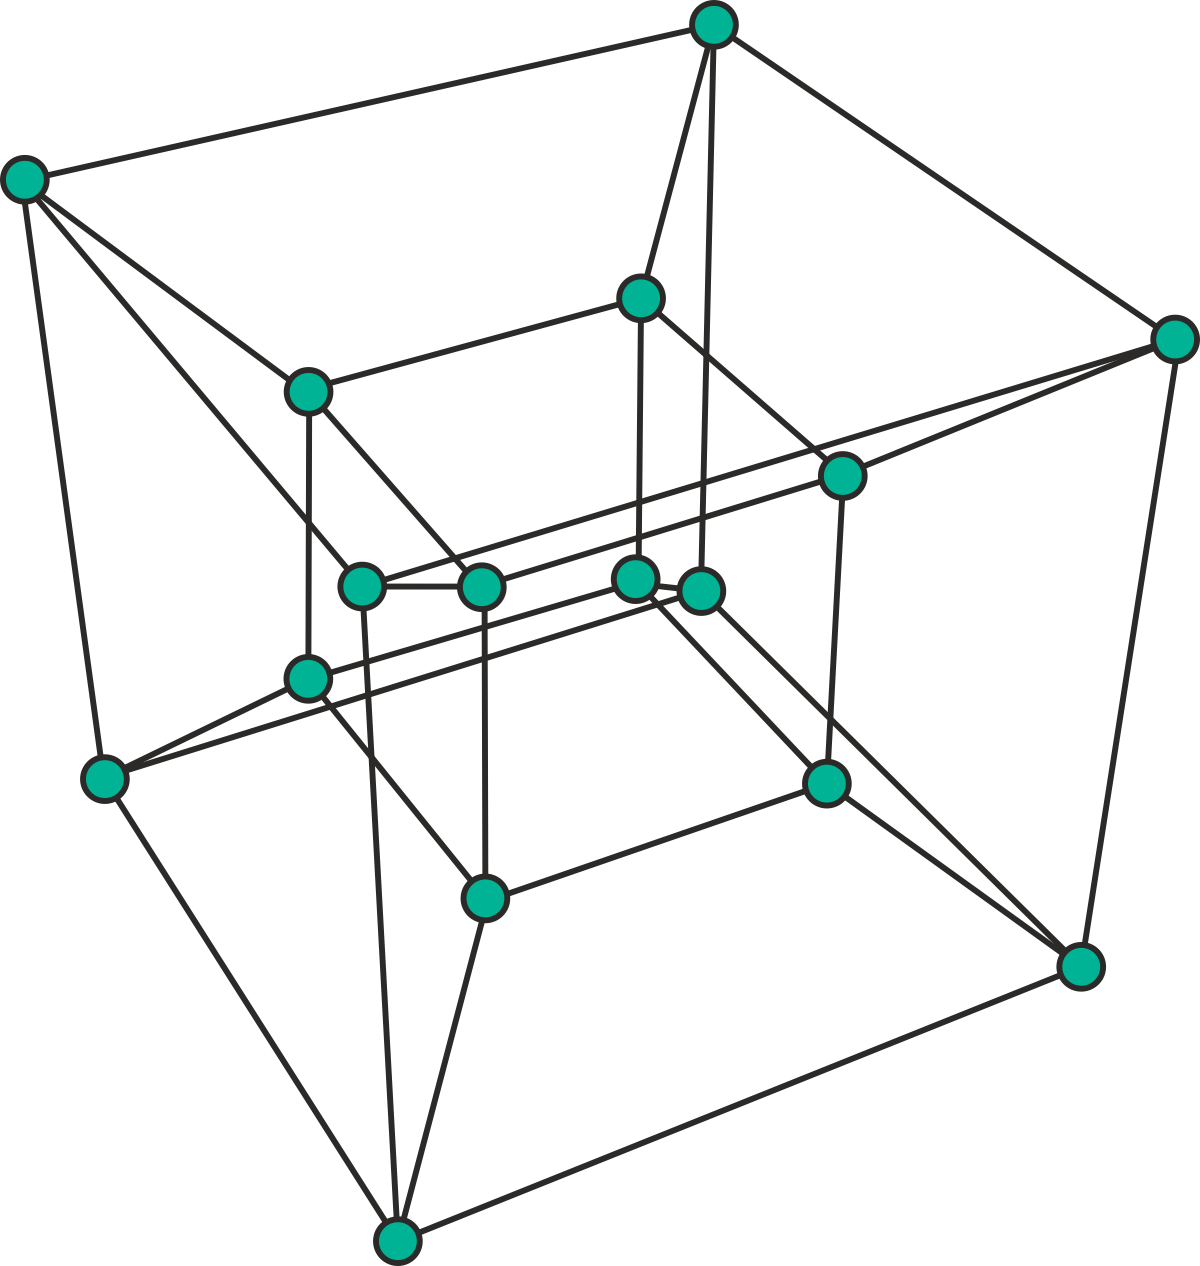
\includegraphics[width=20mm]{images/Fig_1_7_10.png}
    \vspace{-4mm}
\end{wrapfigure}
10К. В базисе $1s$ атомных орбиталей определите электронное строение (энергии и кратности вырождения всех молекулярных орбиталей) произвольной хюккелевской системы c $2^n$ центрами, где $n=0, 1, 2,\ldots$ относящейся к ряду гиперкубов: 0-куб ($n=0$, изолированный центр), 1-куб ($n$ = 1, линейная система из 2 центров), 2-куб ($n$ = 2, квадрат), 3-куб ($n$ = 3, куб), 4-куб ($n$ = 4, тессеракт) и т.д. Двухмерная проекция тессеракта приведена на рисунке справа. Определите также полную электронную энергию описанной в задаче системы для произвольного $n$. Ответ не должен содержать символ суммирования.
\par
\begin{wrapfigure}{r}{20mm} %this figure will be at the right
    \centering
    \vspace{-9mm}
    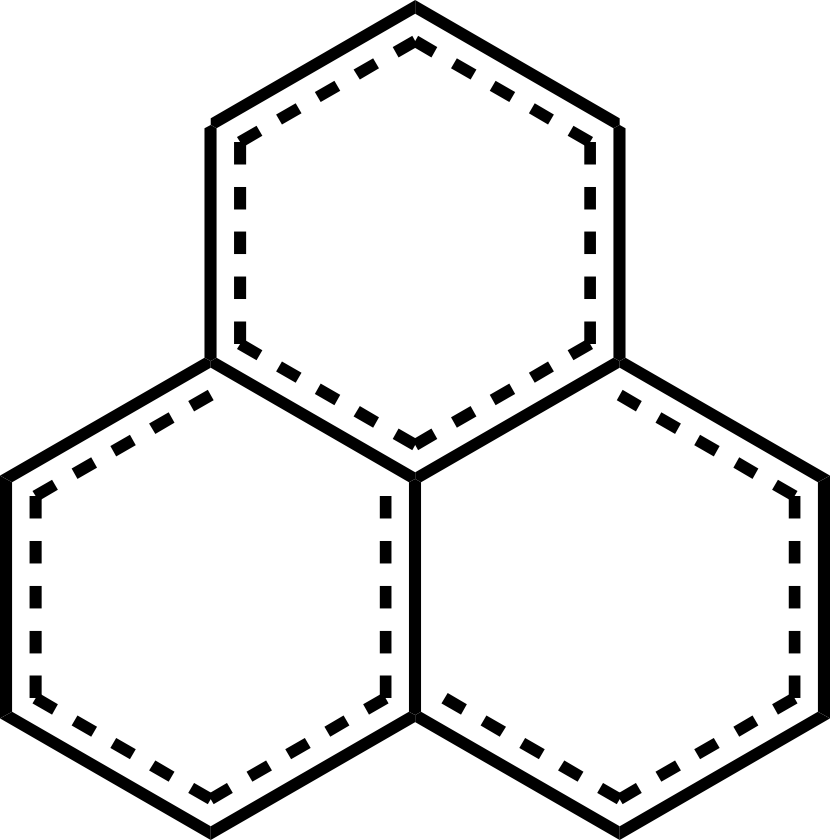
\includegraphics[width=16mm]{images/Fig_1_7_11.png}
    \vspace{-7mm}
\end{wrapfigure}
11. Определите электронное строение $\pi$-системы феналенила, структура которого приведена на рисунке. Сравните результат с теорией возмущений.
\par
12К. Определите поляризацию самой коротковолновой линии в~спектре поглощения $\pi$-системы пентадиенильного радикала.
\par
\begin{wrapfigure}{r}{30mm} %this figure will be at the right
    \centering
    \vspace{-9mm}
    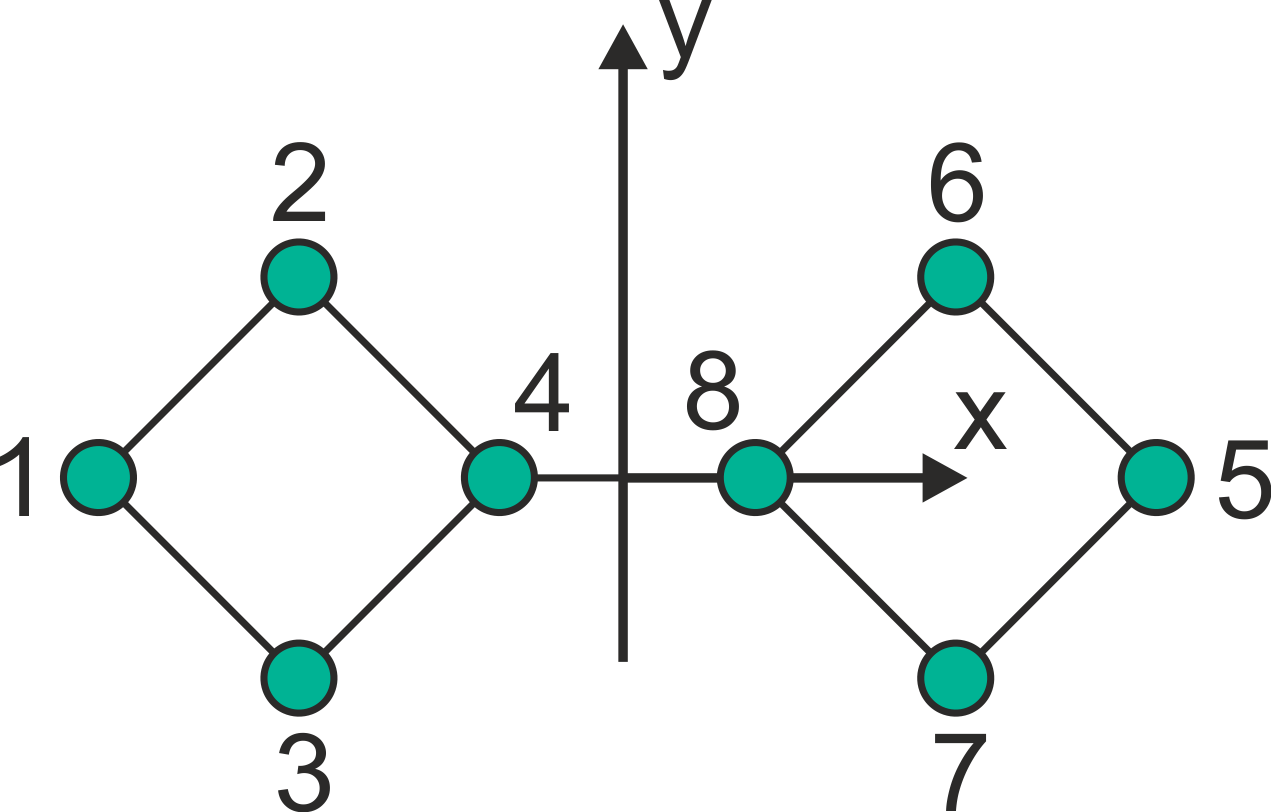
\includegraphics[width=27mm]{images/Fig_1_7_13.png}
    \vspace{-6mm}
\end{wrapfigure}
13К. Определите энергетические уровни и основной терм хюккелевской системы, изображенной на рисунке, в базисе $2p_z$ орбиталей. Все резонансные интегралы одинаковые.
\par
\setmainfont{Noto Serif}
\setsansfont{Noto Sans}
\setmonofont{Noto Sans Mono}
\setstretch{1.35}
\hyphenation{ма-те-ма-ти-ка вос-ста-нав-ли-вать}


\section{Специальные хюккелевские системы}

1С. Определите основной терм $\pi$-системы циклобутадиена.
\par
2. Определите число разрешенных электрических дипольных переходов в~линейном радикале с $n$ центрами. Сколько разрешенных переходов имеют различную энергию?
\par
3С. Определите энергию высшей занятой молекулярной орбитали циклической системы с $n$ центрами ($n = 4k$, $n = 4k + 2$) при введении одного индуктивного заместителя $-\text{CH}_3$ группы.
\par
\begin{wrapfigure}{r}{45mm} %this figure will be at the right
    \centering
    \vspace{-4mm}
    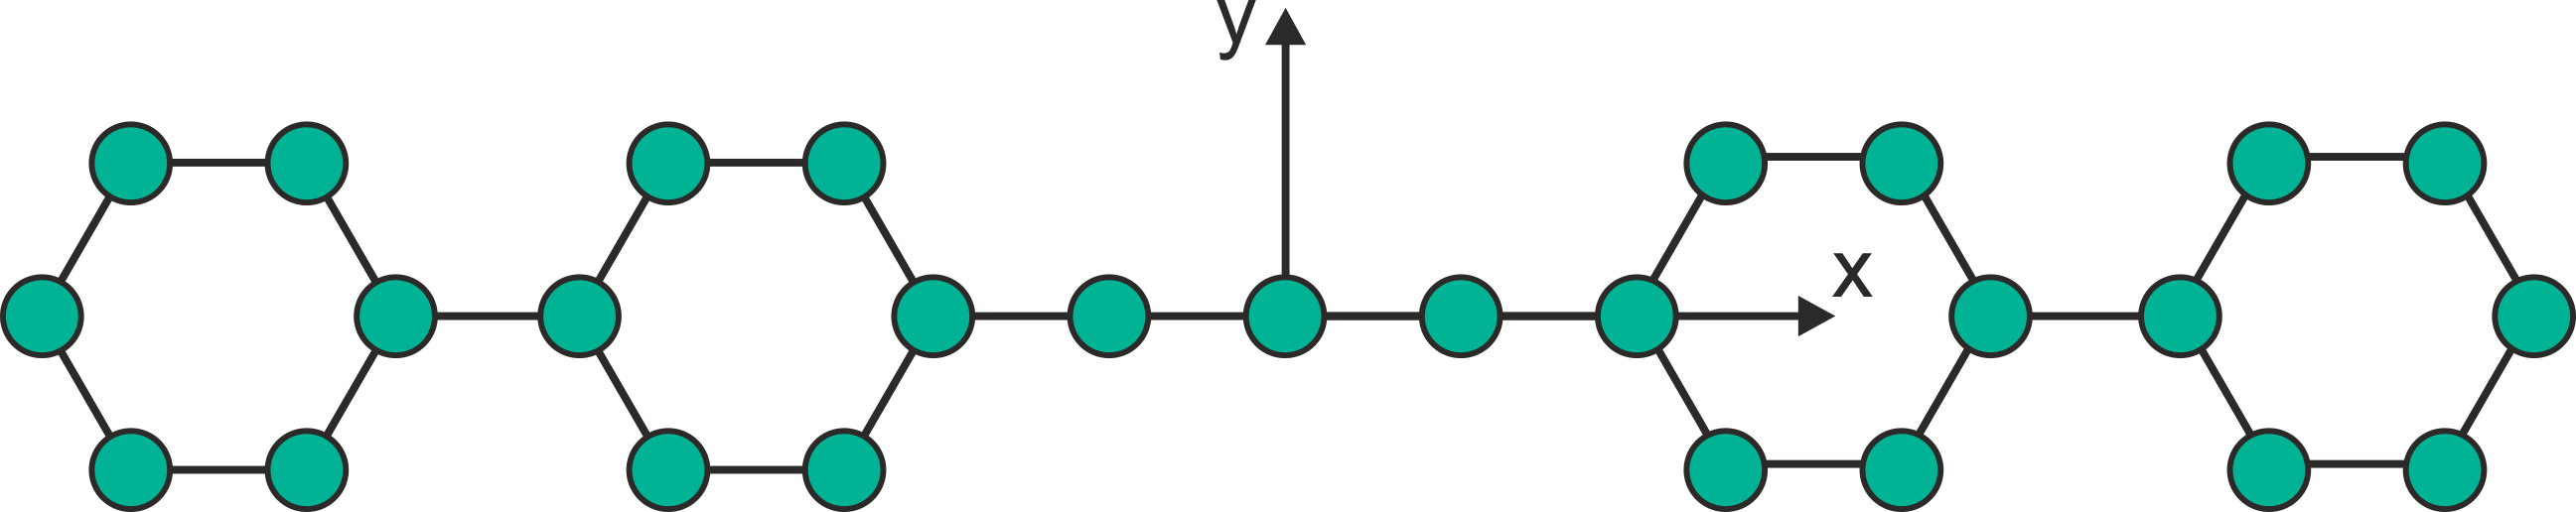
\includegraphics[width=45mm]{images/Fig_1_8_4.png}
    \vspace{-6mm}
\end{wrapfigure}
4С. Определите поляризацию электрического дипольного перехода между молекулярной орбиталью неспаренного электрона и~разрыхляющей молекулярной орбиталью с самой большой энергией для хюккелевской системы, изображенной на рисунке, в базисе $2p_z$ орбиталей.
\par
5. Используя метод Хюккеля качественно опишите электронное строение бесконечной линейной $\pi$-системы. Чему равно расстояние между энергетическими уровнями с максимальной и минимальной энергией?
\par
\begin{wrapfigure}{r}{30mm} %this figure will be at the right
    \centering
    \vspace{-7mm}
    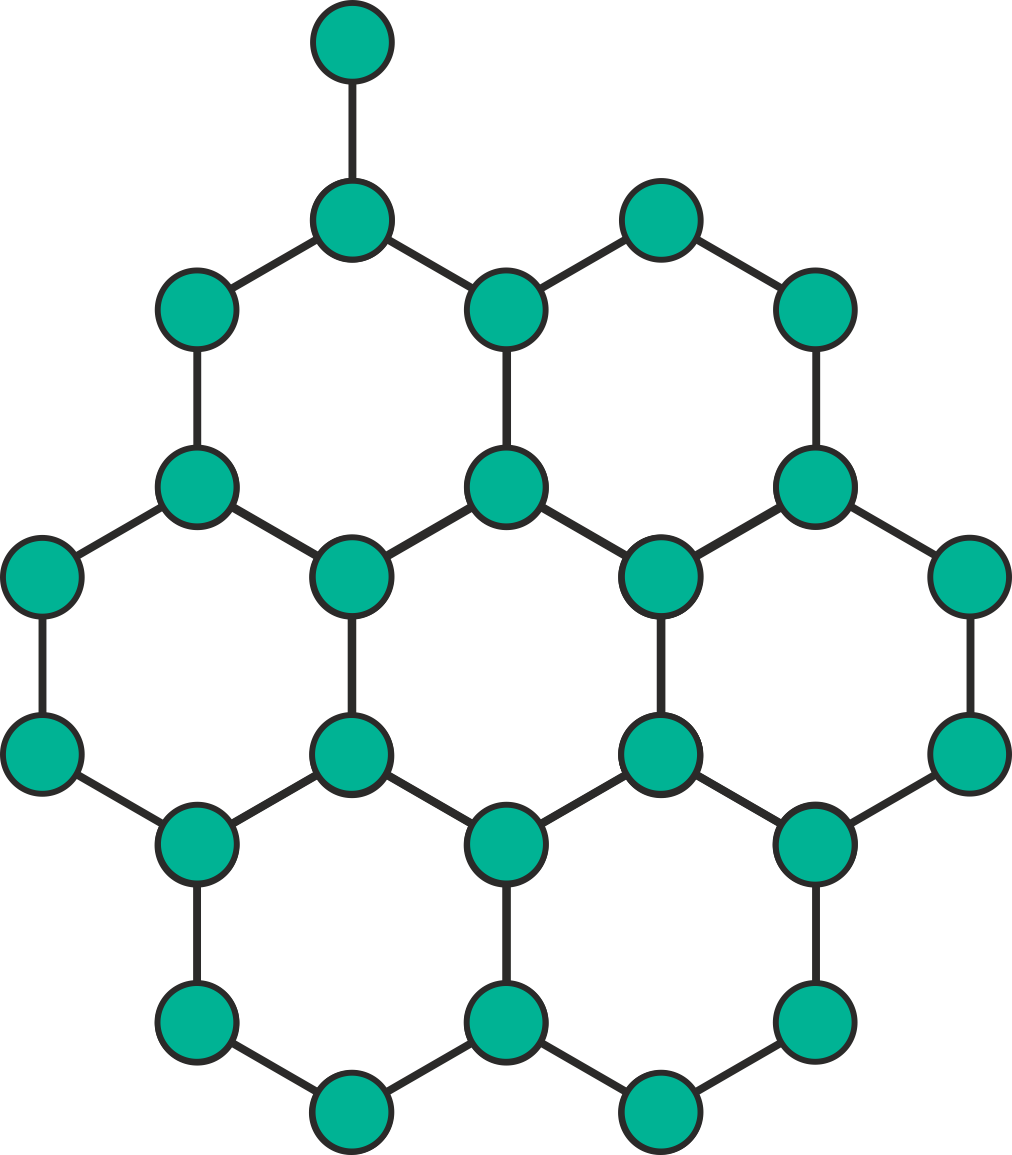
\includegraphics[width=17mm]{images/Fig_1_8_6.png}
    \vspace{-8mm}
\end{wrapfigure}
6С. Определите распределение спиновой плотности для $\pi$-системы, изображенной на рисунке справа. 
\par
7. Определите порядок $\pi$-связи между соседними центрами в~циклической системе с $n= 4k + 2$ центрами.
\par
8. Можно ли с помощью спектра поглощения определить квадратную или прямоугольную геометрию имеет $\pi$-система циклобутадиена? Все резонансные интегралы считать одинаковыми.
\par
9. Определить, какая из трех структур: (1) линейная, (2) угловая, (3) циклическая более устойчива для частиц $\text{H}_3$, $\text{H}_3^+$, $\text{H}_3^-$. В каждом случае определить распределение спиновой плотности и порядок связи.
\par
\begin{wrapfigure}{r}{36mm} %this figure will be at the right
    \centering
    \vspace{2mm}
    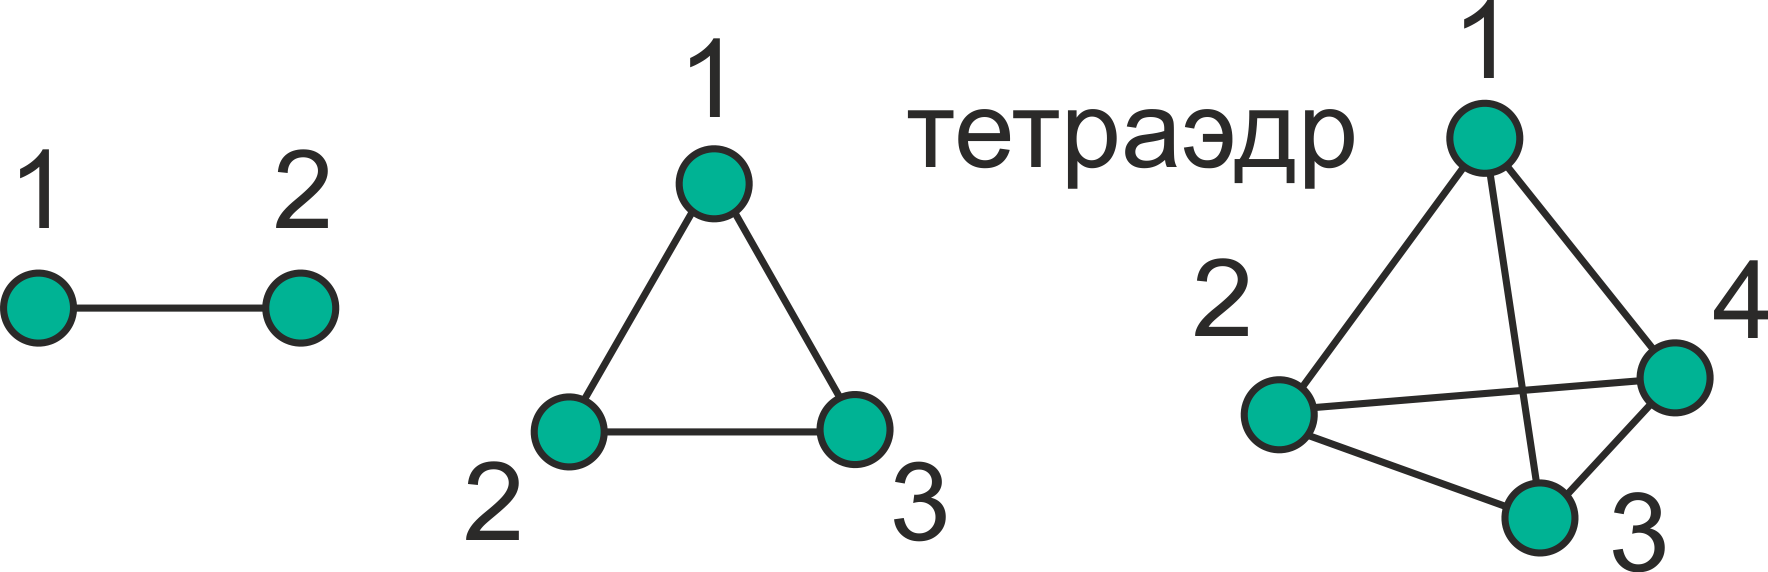
\includegraphics[width=34mm]{images/Fig_1_8_11.png}
    \vspace{-1mm}
\end{wrapfigure}
10К. Помимо циклических и альтернантных, к системам специального типа относятся также полносвязанные хюккелевcкие системы, в которых каждый центр связан с каждым. Три простейших примера таких систем изображены на рисунке. Используя приведенные примеры, экстраполируйте полученный для них ответ и~изобразите схему энергетических уровней для полносвязанной системы с~$n$~центрами. Определите также полную электронную энергию ее $\pi$-системы.
\par
\begin{wrapfigure}{r}{36mm} %this figure will be at the right
    \centering
    \vspace{-7.4ex}
    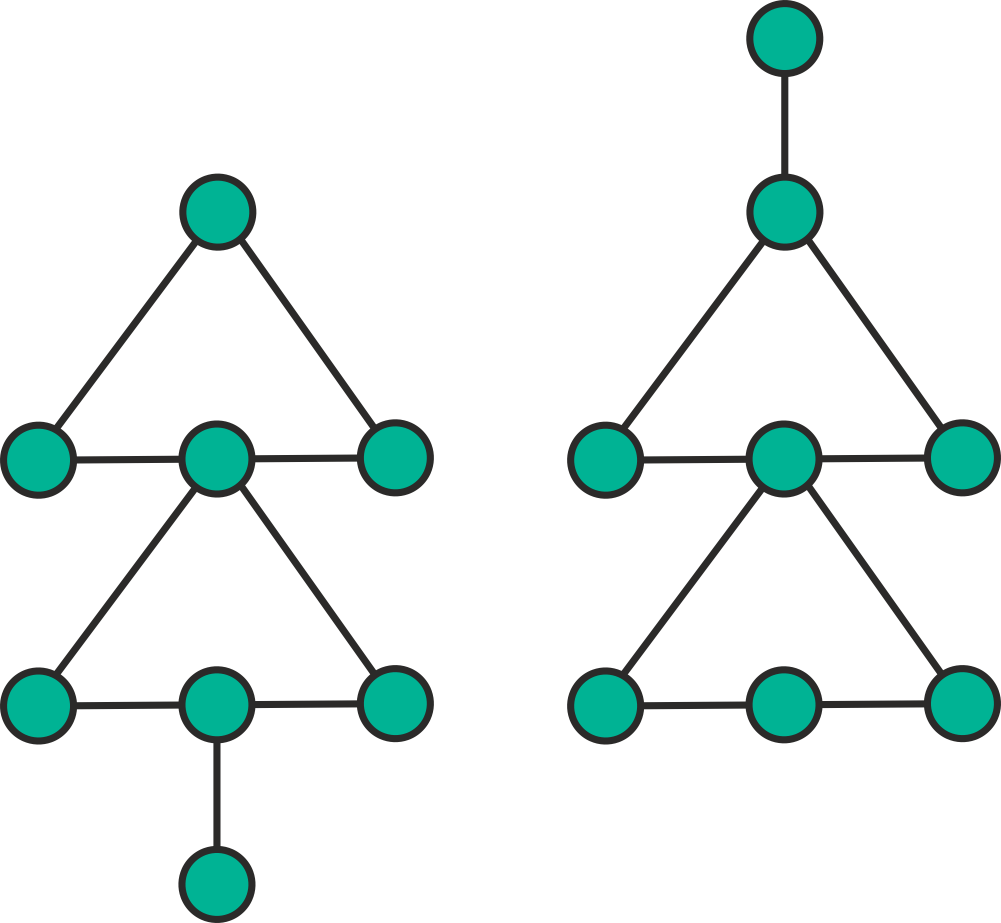
\includegraphics[width=19mm]{images/Fig_1_8_9.png}
    \vspace{-3ex}
\end{wrapfigure}
11. Определить распределение спиновой плотности в радикале, который имеет строение елочки. Рассмотрите два случая, изображенные на рисунке: (1)~елочка с ножкой, считая при этом, что резонансный интеграл с~самым нижним центром елочки равен $\sqrt{2}\beta$, (2) елочка со~звездочкой.
\par
\setmainfont{Noto Serif}
\setsansfont{Noto Sans}
\setmonofont{Noto Sans Mono}
\setstretch{1.35}
\hyphenation{ма-те-ма-ти-ка вос-ста-нав-ли-вать}


\section{Применение теории возмущений}
1. Определите изменение порядка $\pi$-связи в молекуле этилена при введении в~его $\pi$-систему метильной группы.
\par
2С. Используя теорию возмущений определите вид нижней по энергии молекулярной орбитали в молекуле нафталина.
\par
3С. Определите изменение полной электронной энергии $\pi$-системы циклобутадиена, при изменении геометрии молекулы с плоской квадратной на~прямоугольную. Считать, что при таком искажении длины соответствующих связей изменились на 0,1 относительно неискаженной геометрии.
\par
4. Используя теорию возмущений определите распределение спиновой плотности в~анион-радикале п-терфенила.
\par
\begin{wrapfigure}{r}{36mm} %this figure will be at the right
    \centering
    \vspace{-7ex}
    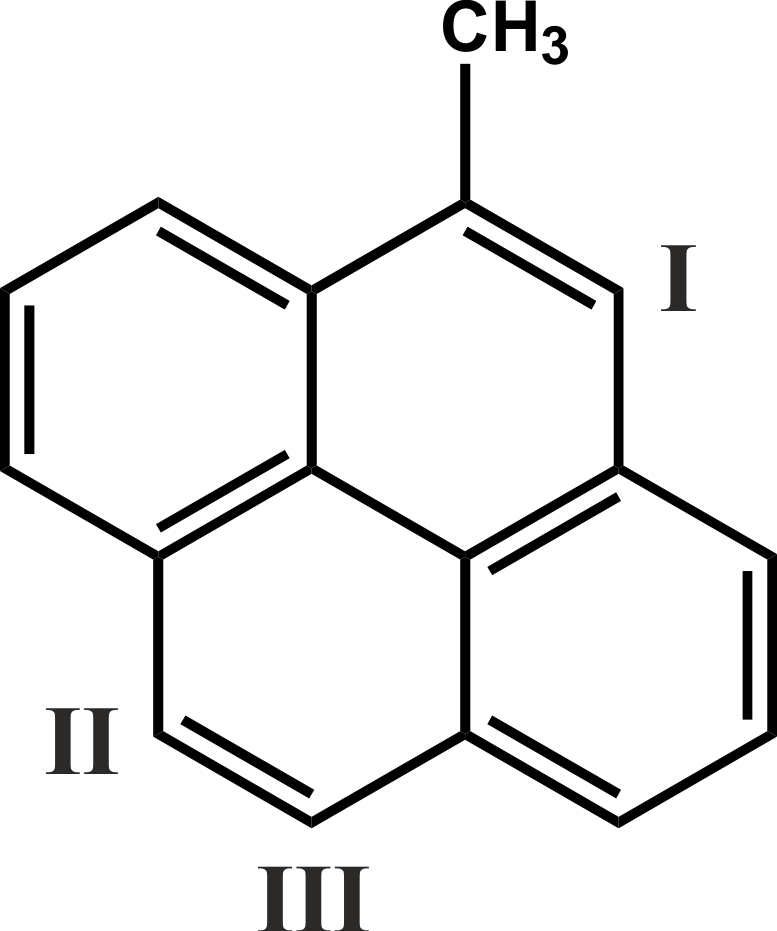
\includegraphics[width=20mm]{images/Fig_1_9_6.png}
    \vspace{-6ex}
\end{wrapfigure}
5К. В первом порядке теории возмущений определите преимущественное направление (центры I, II или III, см.~рисунок) электрофильного ароматического замещения в 4-метилпирене, $\xi$ = $-$0,1.
\par
6. Рассчитать распределение спиновой плотности в анион- и катион-радикале дурола (1,2,4,5-тетраметилбензола). Как изменится энергия и поляризация самого длинноволнового электрического дипольного перехода при переходе от бензола к дуролу?
\par
7. Используя теорию возмущений сравнить относительную устойчивость изомерных $\pi$-систем антрацена и фенантрена.
\par
8С. Определить направление преимущественного нуклеофильного ароматического замещения в 1-метил-2-трифторметил-циклобутадиене.
\par
\begin{wrapfigure}{r}{30mm} %this figure will be at the right
    \centering
    \vspace{-4ex}
    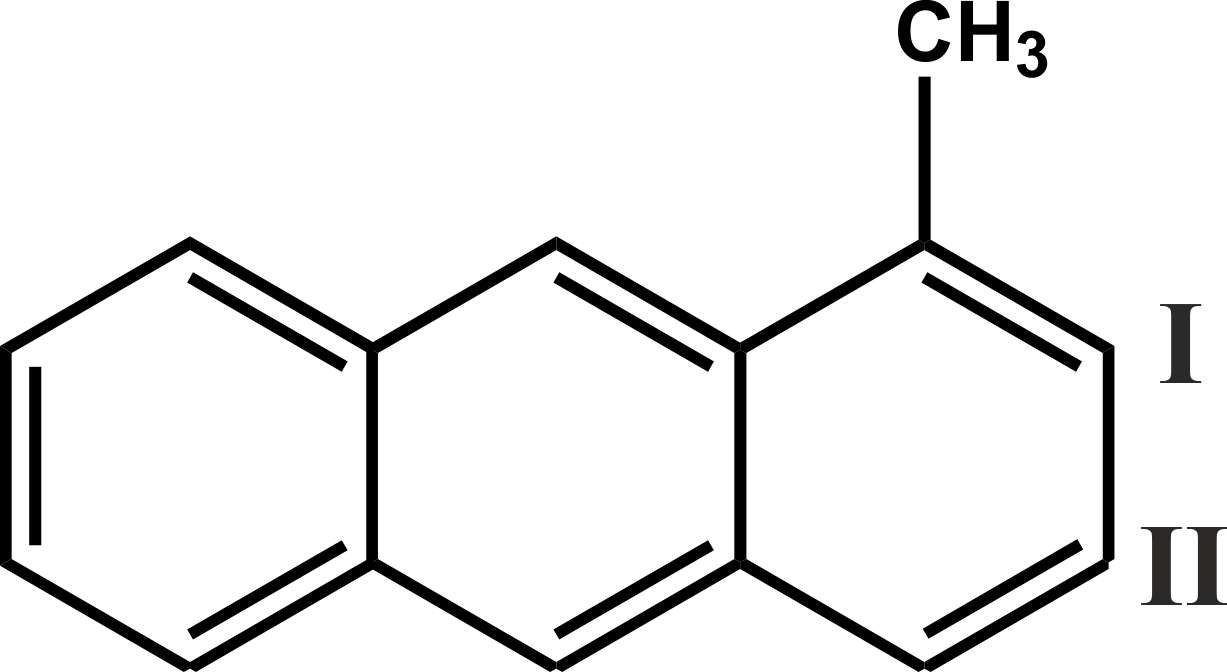
\includegraphics[width=27mm]{images/Fig_1_9_9.png}
    \vspace{-3ex}
\end{wrapfigure}
9К. В первом порядке теории возмущений определите преимущественное направление (центры I или II, см.~рисунок) нуклеофильного ароматического замещения (R$^-$) в~1-метилантрацене, $\xi$ = $-$0,1.
\par
10. В первом порядке теории возмущений определите преимущественное направление нуклеофильного и электрофильного ароматического замещения в~молекуле 4-трифторметилтолуола, $\xi_{\text{CH}_3}$ = $-$0,1, $\xi_{\text{CF}_3}$ = +0,3.
\par
\begin{wrapfigure}{r}{30mm} %this figure will be at the right
    \centering
    \vspace{-3ex}
    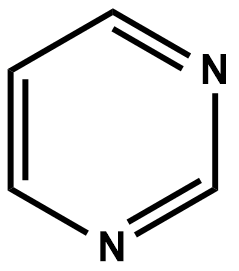
\includegraphics[width=10mm]{images/Fig_1_9_11.png}
    \vspace{-4ex}
\end{wrapfigure}
11Т. Опишите подходы к описанию электронного строения $\pi$-сопряженных соединений, имеющих в своей структуре один или несколько гетероатомов. В качестве примера рассчитайте изменение спиновой плотности в катион-радикале пиримидина, строение которого приведено на рисунке.
\par
12. Определите направление преимущественного электрофильного замещения для молекулы резорцина (1,3-дигидроксибензол). Считайте, что кулоновский интеграл для $2p_z$ атомной орбитали кислорода равен $\alpha_O=\alpha_C+1,2\beta$, резонансные интегралы для связи С–O равны $1,1\beta$.
\par
13. Определить преимущественный продукт одновременного радикального замещения водорода в бензоле двумя одинаковыми радикалами.
\par
14. Можно ли различить изомеры дважды дейтерированного бензола по энергии самой коротковолновой полосы поглощения $\pi$-системы?
\par
\begin{wrapfigure}{r}{30mm} %this figure will be at the right
    \centering
    \vspace{-4ex}
    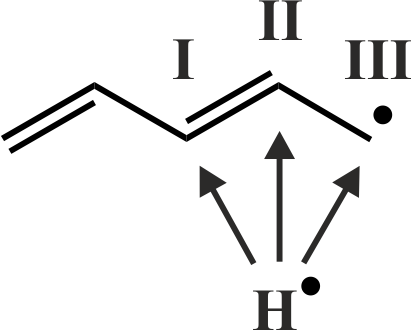
\includegraphics[width=18mm]{images/Fig_1_9_15.png}
    \vspace{-4ex}
\end{wrapfigure}
15К. Определите направление преимущественного присоединения (центры I, II или III, см. рисунок) атома водорода к $\pi$-системе пентадиенильного радикала.
\par


\chapter[Электронное строение координационных соединений.\\Спектроскопические методы исследования вещества]{\texorpdfstring{Электронное строение\\координационных соединений.\\Спектроскопические методы исследования вещества}{Электронное строение координационных соединений. Спектроскопические методы исследования вещества}}
\thispagestyle{empty}

\setmainfont{Noto Serif}
\setsansfont{Noto Sans}
\setmonofont{Noto Sans Mono}
\setstretch{1.35}

\section{Правила Вудворда-Хоффмана}
1С. Постройте корреляционную диаграмму образования хюккелевской системы, имеющей строение треугольной призмы, из двух одинаковых треугольных хюккелевских систем. Определите чему равно изменение полной электронной энергии в ходе данной реакции. Используйте базис $1s$ атомных орбиталей.
\par
\begin{wrapfigure}{r}{28mm} %this figure will be at the right
    \centering
    \vspace{-1mm}
    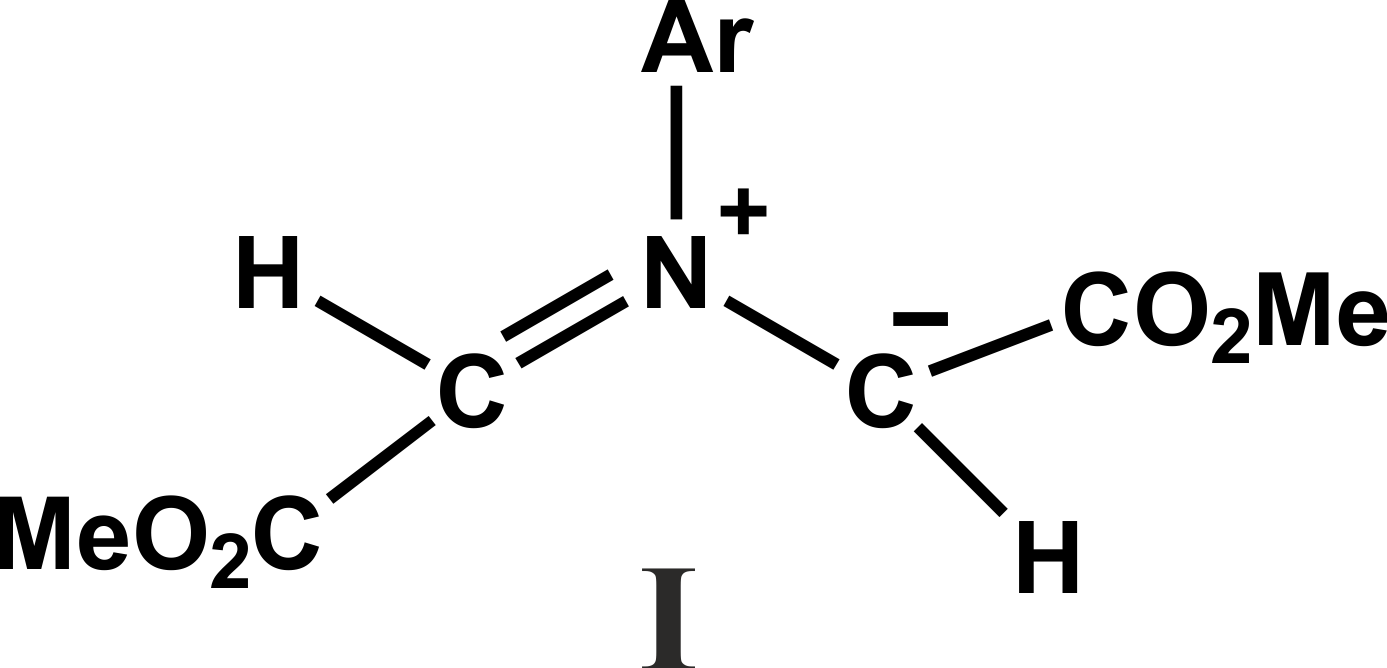
\includegraphics[width=28mm]{images/Fig_2_1_2.png}
    \vspace{0mm}
\end{wrapfigure}
2К. Определите по какому механизму (кон- или дисротаторный) протекает реакция термической циклизации транс-азометинового илида I, изображенного на рисунке. Укажите стереохимию продукта реакции и постройте корреляционную диаграмму. Соединение I изоэлектронно аллил-аниону, $\text{Ar}=\text{C}_6\text{H}_4-\text{OCH}_3$.
\par
%$\leftrightarrows$
3. Постройте корреляционную диаграмму цис-транс-изомеризации производных этилена.
\par
4С. Постройте корреляционную диаграмму реакции термического циклоприсоединения бутадиена и этилена в $4\pi_s$ + $2\pi_s$ топологии. Используя правила Вудворда-Хоффмана рассмотрите протекание реакции в других топологиях. Можно ли в этих случаях построить корреляционную диаграмму?
\par
5Т. Каким образом протекает реакция $\text{H}_2$ + $\text{D}_2$ $\rightleftarrows$ 2$\text{HD}$:  термически или фотохимически? Постройте корреляционную диаграмму.
\par
\begin{wrapfigure}{r}{34mm} %this figure will be at the right
    \centering
    \vspace{-1.9mm}
    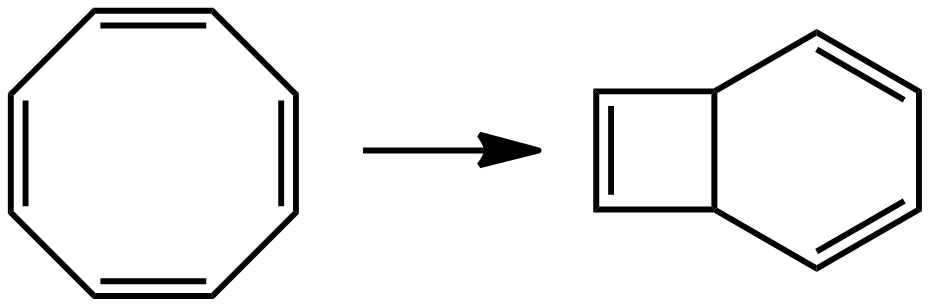
\includegraphics[width=28mm]{images/Fig_2_1_5.png}
    \vspace{-3.4mm}
\end{wrapfigure}
6С. Постройте корреляционную диаграмму изомеризации  циклооктатетраена по дисротаторному механизму согласно реакции, приведенной на рисунке. Может ли данная реакция протекать термически?
\par
\begin{wrapfigure}{r}{34mm} %this figure will be at the right
    \centering
    \vspace{-1mm}
    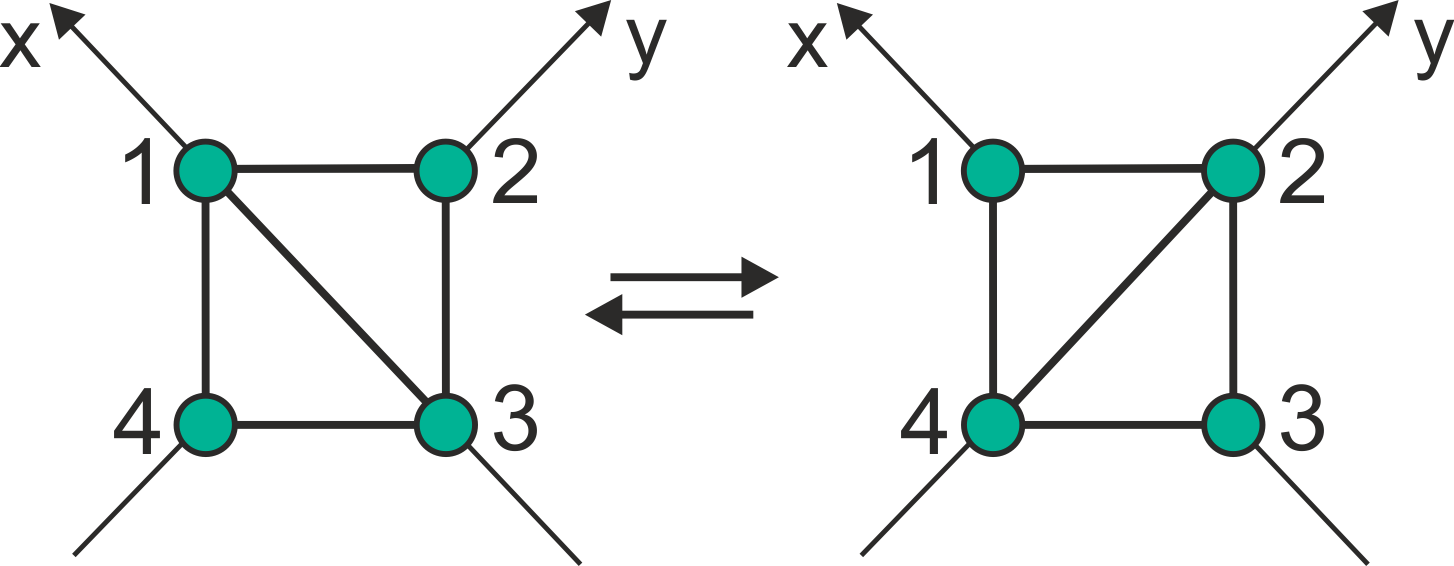
\includegraphics[width=34mm]{images/Fig_2_1_7.png}
    \vspace{-3.5mm}
\end{wrapfigure}
7. Постройте корреляционную диаграмму реакции изомеризации, изображенной на рисунке справа. Разрешена или запрещена данная реакция при термическом протекании? Чему равно изменение полной электронной энергии в ходе данной реакции?
\par
8Т. Сформулируйте правила Вудворда-Хоффмана для реакции циклоприсоединения Дильса-Альдера в общем случае.
\par
9. Определить термически или фотохимически разрешена реакция присоединения атома водорода к молекуле водорода. Предполагается образование циклической молекулы при сближении $\text{H}$ и $\text{H}_2$ перпендикулярно направлению связи $\text{H}$$-$$\text{H}$. Определите симметрию молекулярных орбиталей продуктов и~реагентов реакции в терминах неприводимых представлений сохраняющейся группы симметрии. В случае фотохимического механизма предварительно определить, разрешен ли электрический дипольный переход в предполагаемое возбужденное состояние.
\par
\begin{wrapfigure}{r}{17.5mm} %this figure will be at the right
    \centering
    \vspace{-3mm}
    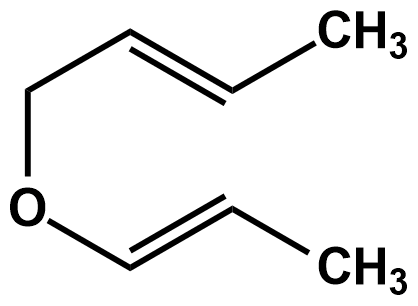
\includegraphics[width=17.5mm]{images/Fig_2_1_10.png}
    \vspace{-5mm}
\end{wrapfigure}
10С. Исходя из правил Вудворда-Хоффмана опишите механизм протекания [3,3]-сигматропного сдвига (перегруппировка Кляйзена) в производном 2,6-октадиена, который изображен на рисунке, в случае ее термического протекания. Укажите стереохимию продукта реакции.
\par
11. Определите разрешена ли реакция присоединения $\text{N}$$-$$\text{H}$ к $\text{H}$$-$$\text{H}$ с образованием NH$_3$? Сближение происходит так, что связи $\text{N}$$-$$\text{H}$ и $\text{H}$$-$$\text{H}$ перпендикулярны друг другу. Для атома азота учитывайте только $2p$ атомные орбитали.
\par
12. Реакция циклоприсоединения двух молекул этилена в супра-/супра- топологии запрещена термически. Может ли металл в конфигурации $d^n$ снять этот запрет? Чему равно минимальное и максимальное значение $n$?
\par
13К. Постройте корреляционную диаграмму термического превращения циклооктатетраена в кубан в супра-\,/\,супра- топологии.
\par
\setmainfont{Noto Serif}
\setsansfont{Noto Sans}
\setmonofont{Noto Sans Mono}
\setstretch{1.35}

\section{Теория кристаллического поля}
1С. Определите расщепление электронных уровней основного терма иона $\text{Ti}^{3+}$ ($3d^1$) в октаэдрическом комплексе, в котором расстояния до всех лигандов одинаковые, а заряд одного из лигандов в два раза меньше, чем заряд остальных пяти.
\par
2С. Определите расщепление электронных уровней основного терма центрального атома металла с электронной конфигурацией $3d^1$ в поле лиганда, представляющего собой окружность радиуса $a$, по которой равномерно распределен заряд $Q$.
\par
3С. Определите расщепление электронных уровней основного терма центрального атома металла с электронной конфигурацией $p^2$ в координационном соединении, имеющем квадратное строение.
\par
4. Определите изменение энергии $3d_{z^2}$ орбитали при удалении двух аксиальных лигандов из комплекса иона $\text{Ti}^{3+}$ ($3d^1$), имеющего строение правильной треугольной бипирамиды.
\par
5. Определите расщепление электронных уровней основного терма иона $\text{Ti}^{2+}$ ($3d^2$) в октаэдрическом комплексе.
\par
6С. Используя теорию поля лигандов качественно опишите электронное строение тетраэдрического аминокомплекса металла с конфигурацией $3d^n$.
\par
7С. Объясните, почему коэффициент экстинкции комплекса цис-$\text{[Co(NH}_3)_4\text{Cl}_2]^+$ заметно больше, чем соответствующего транс-изомера.
\par
8. Сравнить относительную возможность протекания реакций замещения в~октаэдрических комплексах по механизму $S_{N}1$ (переходное состояние – квадратная пирамида) и $S_{N}2$ (переходное состояние – пентагональная бипирамида) для электронных конфигураций центрального металла $d^4$, $d^5$, $d^6$. Рассмотреть случаи сильного и слабого поля.
\par
9С. Как расщепляются термы $^4G_g$ и $^4G_u$ в поле тетраэдра?
\par
10. Как будут расщепляться $p$ орбитали в поле двух точечных зарядов $q_1$ и $q_2$, расположенных на оси $х$ на расстоянии $\pm a$ от начала системы координат?
\par
\begin{wrapfigure}{r}{33mm} %this figure will be at the right
    \centering
    \vspace{-3.8mm}
    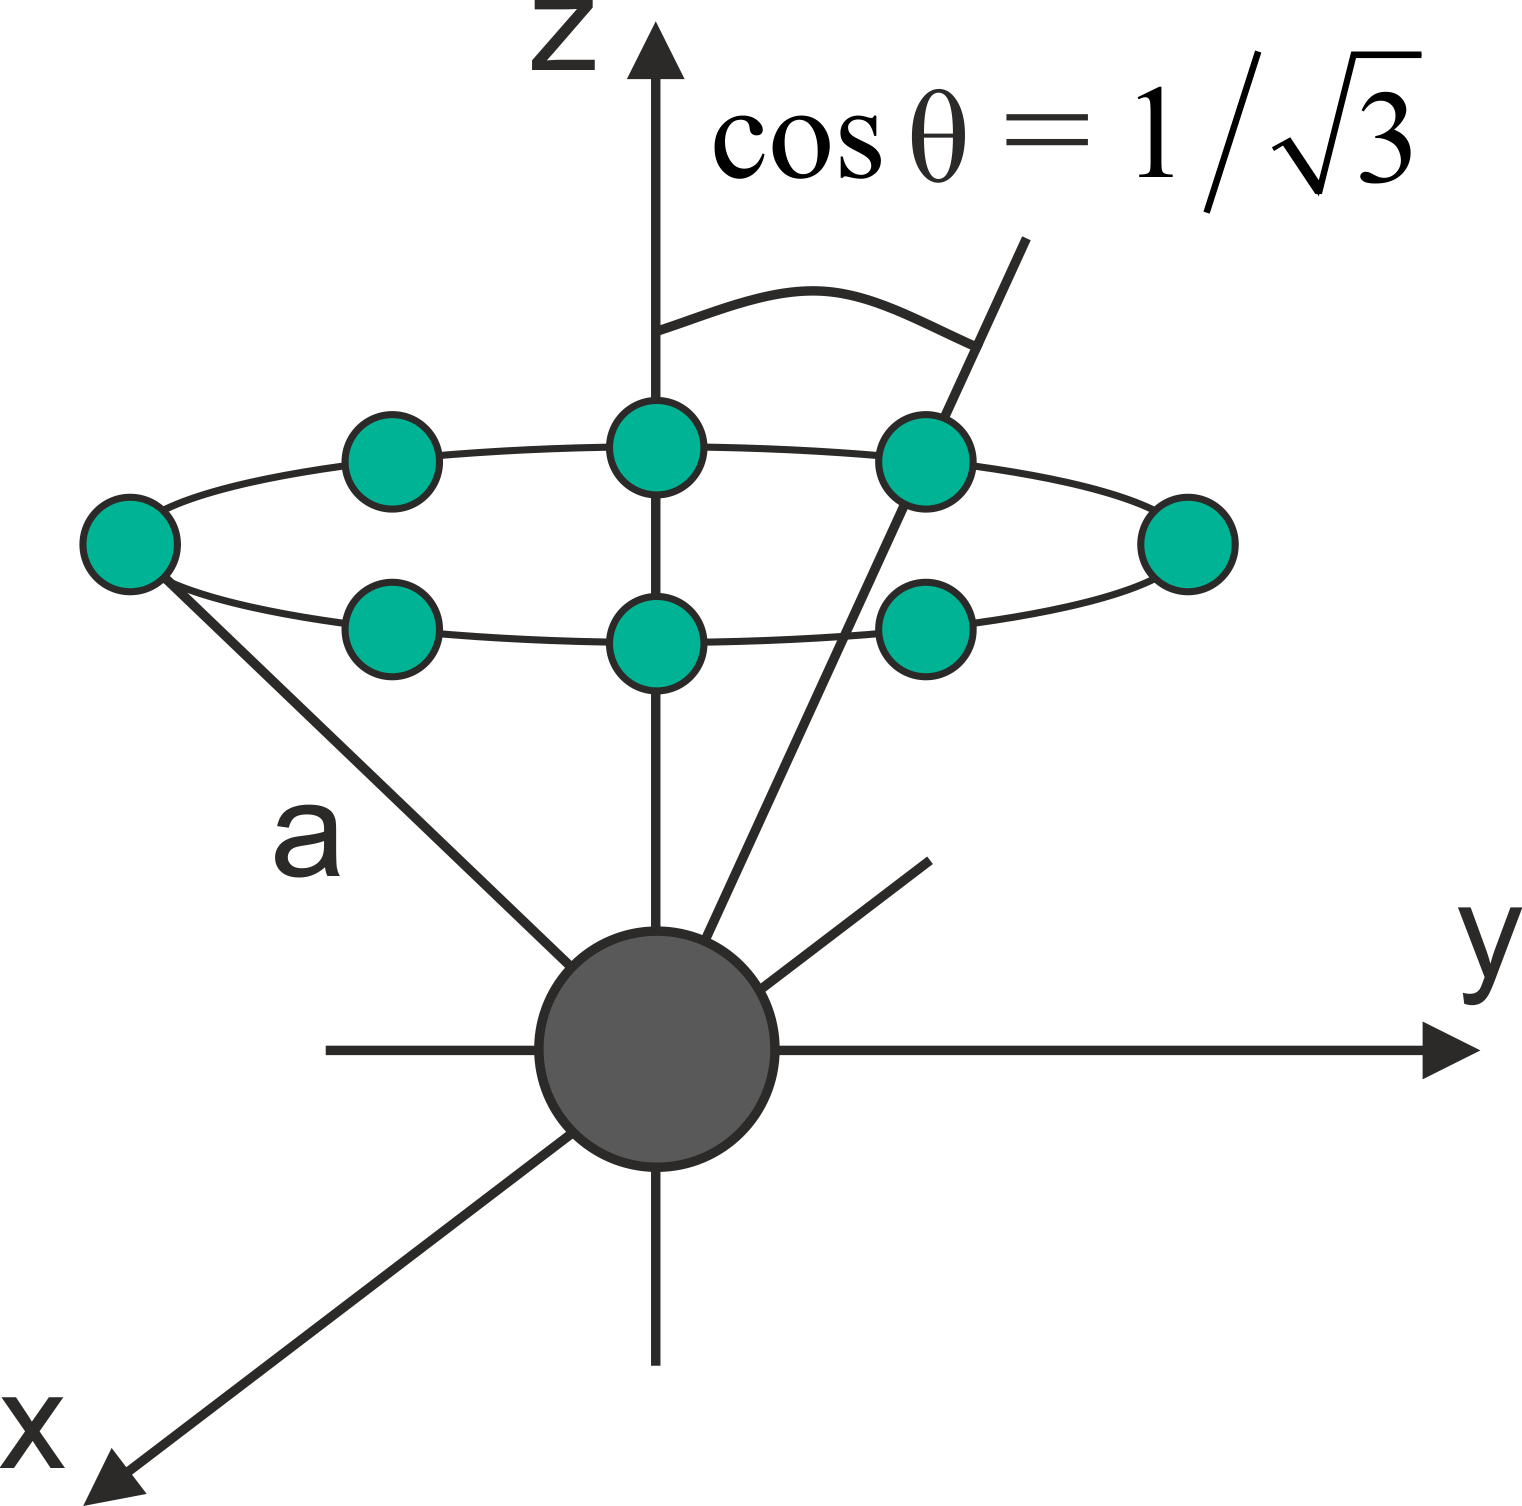
\includegraphics[width=28mm]{images/Fig_2_2_14.png}
    \vspace{-5mm}
\end{wrapfigure}
11К. В структуре цеолитов можно встретить каналы различного размера. Пренебрегая спин-орби-тальным взаимодействием, определите энергию $f_{z^3}$ орбитали иона $\text{Ce}^{3+}$ ($4f^1$), расположенного над восьмичленным кольцом цеолита, как изображено на~рисунке. Лигандные атомы кислорода расположены в~вершинах правильного плоского восьмиугольника. Расстояния от центрального атома до атомов кислорода равны $a$, угол $\theta$ такой, что $\cos\theta=\sqrt{3}/3$. Дополнительные справочные данные приведены ниже.
\\
Некоторые эквивалентные операторы для угловых интегралов с $\textit{Y}_{3m}$:
\vspace{0.1mm}
\begin{equation*}
\begin{aligned}
\widehat L_{60} &= -\frac{1}{2376}\sqrt{\frac{1}{13\pi}}\left( 231\widehat L_z^6-315\widehat L^2\,\widehat L_z^4 +735\widehat L_z^4+105({\widehat L^2})^2\,\widehat L_z^2\,- \right.\\[6pt]
&\quad\qquad\qquad\qquad\ \left. -\,525\widehat L^2\,\widehat L^2_z +294\widehat L^2_z - 5 (\widehat L^2)^3 + 40 (\widehat L^2)^2-60 \widehat L^2 \right);
\\[2pt]
 \widehat L_{64} &= -\frac{1}{1584}\sqrt{\frac{7}{26\pi}}\left( (11\widehat L^2_z - \widehat L^2 -38)(\widehat L^4_++\widehat L^4_-)+(\widehat L^4_++\widehat L^4_-)(11\widehat L^2_z - \widehat L^2 -38) \right); 
\\[6pt]
  \widehat L_{66} &= -\frac{1}{144}\sqrt{\frac{7}{429\pi}}\left(\widehat L^6_++\widehat L^6_-\right); \quad  \widehat L_{44} =\frac{1}{264}\sqrt{\frac{7}{10\pi}} \left( \widehat L_+^4 + \widehat L_-^4  \right);
\\[6pt]
\widehat L_{40} &= \frac{1}{1320}\sqrt{\frac{1}{\pi}}\left( 35\widehat L_z^4-30\widehat L_z^2 \widehat L^2+25\widehat L_z^2-6\widehat L^2+3 (\widehat L^2)^2 \right); 
\\[6pt]
\widehat L_{20} &= -\frac{1}{18}\sqrt{\frac{1}{5\pi}}\left(3\widehat L_z^2-\widehat L^2\right);
\end{aligned}
\end{equation*}
\\
Вид некоторых сферических гармоник $\textit{Y}_{6m}$:
\begin{equation*}
 \begin{aligned}
&\textit{Y}_{60} =\frac{1}{32}\sqrt{\frac{13}{\pi}}\left(231 \cos^6{\theta}-315\cos^4{\theta}+105\cos^2{\theta}-5 \right); 
\\[6pt]
&\textit{Y}_{6\pm4} =\frac{3}{32}\sqrt{\frac{91}{2\pi}} \left( 11\cos^2{\theta}-1\right) \sin^4 {\theta} \, e^{\,\pm4i\phi}; \quad \textit{Y}_{6\pm6}=\frac{1}{64}\sqrt{\frac{3003}{\pi}} \sin^6 {\theta} \, e^{\,\pm6i\phi};\,\,\quad\quad
 \end{aligned}
\end{equation*}
\par
12. Какого типа полосы переноса заряда следует ожидать для координационных соединений $\text{Fe}^{2+}$ и $\text{Fe}^{3+}$ с органическими лигандами?
\par
13. Качественно и количественно определить, как изменится расщепление $d$~орбиталей в поле лигандов квадратной конфигурации, если (1) одну из сторон квадрата повернуть на 90º, (2) каждый лиганд поделить пополам и два получившихся квадрата сдвинуть вверх и вниз, то есть превратить квадрат в~куб. Для обоих случаев нарисовать корреляционные диаграммы.
\par
14. Определить основной терм для случая электронной конфигурации центрального атома $p^2$ в среднем и сильном поле лигандов, которые расположены в вершинах правильного треугольника.
\par
15К. Качественно изобразите корреляционную диаграмму слабое кристаллическое поле $\leftrightarrow$ сильное кристаллическое поле для триплетных термов иона металла с электронной конфигурацией $3d^2$ в тетраэдрическом окружении.
\par
\setmainfont{Noto Serif}
\setsansfont{Noto Sans}
\setmonofont{Noto Sans Mono}
\setstretch{1.35}

\section{Электронная спектроскопия}
1. Студенту ФЕН НГУ вручили нитку из молекул полистирола и предложили построить такую геометрию эксперимента по исследованию анизотропии люминесценции, чтобы установить расположение бензольных колец. Каким образом необходимо провести данный эксперимент? Считать, что бензол прикреплен перпендикулярно направлению цепи, а цепь ориентирована строго вдоль нитки.
\par
2С. Известны квантовые выходы и времена флуоресценции ($\phi_f^0$, $\tau_f^0$) и фосфоресценции ($\phi_p^0$, $\tau_p^0$) некоторого люминофора. Молекула Q тушит возбужденные синглетные и триплетные состояния люминофора с одинаковой константой скорости $k$. Получите выражение, аналогичное уравнению Штерна-Фольме-ра, для зависимости квантового выхода фосфоресценции $\phi_p$ от концентрации тушителя Q.
\par
\begin{wrapfigure}{r}{30mm} %this figure will be at the right
    \centering
    \vspace{-4.2ex}
    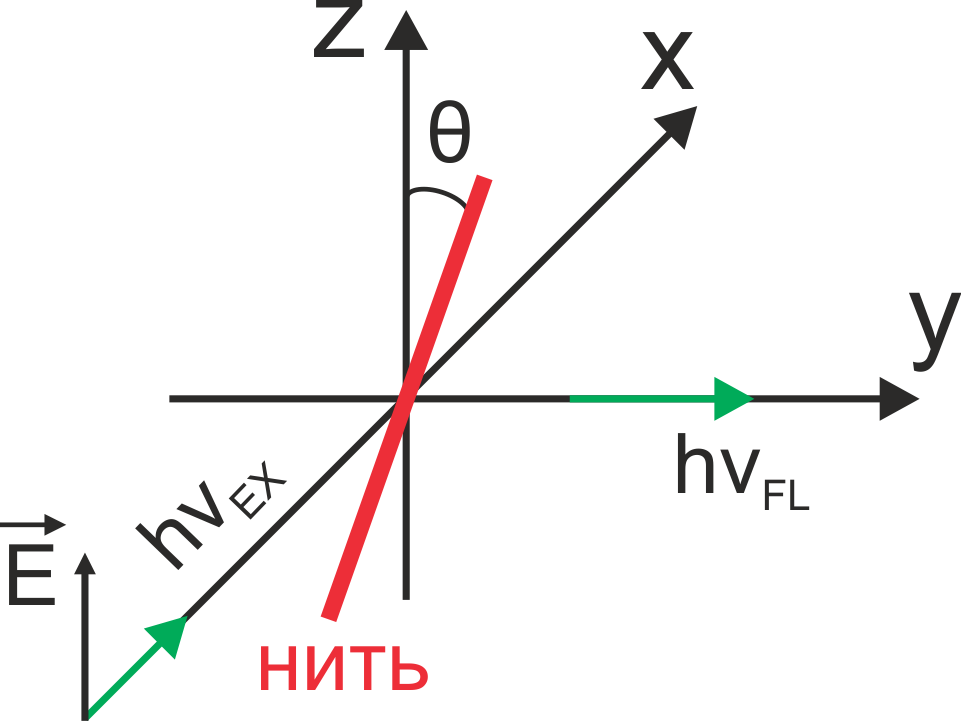
\includegraphics[width=28mm]{images/Fig_2_3_3.png}
    \vspace{-5ex}
\end{wrapfigure}
3С. Определить степень поляризации люминесценции для геометрии опыта, показанной на рисунке. Образцом является тонкая нить, в которой дипольные моменты всех молекул направлены вдоль оси нити. Нить лежит в плоскости $xz$ под углом $\theta$ к оси $z$.
\par
4К. Определите число разрешенных электрических дипольных переходов в молекуле аммиака. Между какими электронными состояниями они протекают?
\par
5С. Определите степень поляризации люминесценции вдоль оси $x$ твердого образца, в котором нет диффузии, если лазерное возбуждающее излучение распространяется по оси $y$, а электрическое поле лазерного излучения отклонено на угол $\theta$ от оси $z$.
\par
6К. Молекулярный кислород обладает значительной растворимостью во многих органических растворителях и воде, а также является тушителем люминесценции. Считая, что точность измерения времени жизни возбужденного состояния $\tau$ составляет 3\%, определите, начиная с какого $\tau$ растворенный кислород начинает оказывать влияние на экспериментально определенное время жизни возбужденного состояния некого люминофора в воде. Растворимость кислорода в воде равна 1,3$\cdot$10$^{-3}$ М, диффузионная константа скорости равна 10$^{10}$ М$^{-1}$$\cdot$с$^{-1}$.
\par
7Т. В какой из молекул (бензол, нафталин, антрацен) расщепление между уровнями $S_1$ и $T_1$ больше?
\par
8. Переход $S_0$ $\rightarrow$ $S_1$ в пиридине поляризован вдоль оси, перпендикулярной плоскости молекулы. Определить поляризацию перехода $S_0$ $\rightarrow$ $T_1$.
\par
9С. Каждая молекула донора D жестко связана с акцептором A так, что расстояние между ними равно $R_0$, где $R_0$ – радиус Ферстера. Время жизни возбужденного состояния D в отсутствии тушителя равно 1 мкс. В раствор добавлен еще один тушитель B с концентрацией 1 мМ. Определите константу бимолекулярного тушения донора D молекулой B, если квантовый выход люминесценции донора уменьшился в 3 раза по сравнению со случаем отсутствия обоих тушителей.
\par
10С. Определите степень поляризации люминесценции растянутой пленки, в~которой дипольные моменты люминесцирующих молекул могут находиться только в плоскости этой пленки. Возбуждающее лазерное излучение распространяется по оси $y$ и имеет $\sigma$ поляризацию, пленка расположена под углом $\phi$ к оси $z$, детектирование люминесценции происходит по оси $y$.
\par
11С. Квантовые выходы флуоресценции и фосфоресценции некоторого красителя равны по 0,5, а его время жизни флуоресценции составляет 10 нс. Определите константу скорости интеркомбинационной конверсии.
\par
12С. Определите степень поляризации люминесценции образца, в котором люминесцирующие молекулы находятся в жесткой молекулярной матрице, при его облучении двумя световыми потоками: (1) вдоль оси $z$ с поляризацией вдоль оси $y$, (2) вдоль оси $y$ с поляризацией вдоль оси $z$. Регистрация люминесценции производится вдоль оси $x$.
\par
\begin{wrapfigure}{r}{47mm} %this figure will be at the right
    \centering
    \vspace{0mm}
    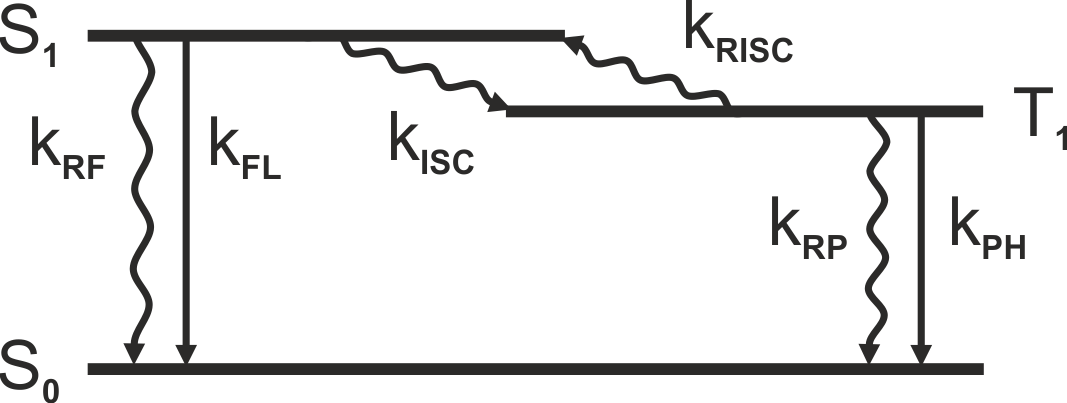
\includegraphics[width=47mm]{images/Fig_2_3_15.png}
    \vspace{-5mm}
\end{wrapfigure}
13К. Одним из способов повышения эффективности органических светодиодов является использование процесса термически активируемой задержанной флуоресценции (TADF). В простейшей трехуровневой TADF системе E-типа протекают процессы, изображенные на рисунке. Получите выражение для квантового выхода задержанной флуоресценции. Покажите, что его величина растет при увеличении $k_{RISC}$. Как вы считаете, с чем связано название процесса TADF?
\par
14К. Тушение кумарина C120 урацилом происходит по динамическому и статическому механизму. Определите динамическую константу тушения $k_q$ и~статическую константу равновесия $K_s$ реакции C120 + Q $\leftrightarrows$ [C120$-$Q], где Q – тушитель, если интенсивность флуоресценции падает в 1,26 раз при использовании 9,5~мМ концентрации тушителя. Время флуоресценции C120 без тушителя равно 5~нс. При концентрации тушителя 20 мM время флуоресценции укорачивается и~оказывается равным 3,85 нс.
\par
15Т. Относительный квантовый выход фосфоресценции нафталина при температуре 77 К зависит от концентрации бензофенона, выступающего в роли тушителя, в соответствии с таблицей, приведенной ниже. Выведите уравнение, описывающее $\phi/ \phi_0$ для данных экспериментальных условий, а также определите радиус тушения.

\begin{center}
\begin{tabular}{ c c c c c c c }

 $C$, M & 0 & 0,08 & 0,16 & 0,24 & 0,32 & 0,40 \\ 
 \hline
 $\phi / \phi_0$ & 1 & 0,65 & 0,45 & 0,23 & 0,19 & 0,13 \\  
\end{tabular}
\end{center}

\par

\setmainfont{Noto Serif}
\setsansfont{Noto Sans}
\setmonofont{Noto Sans Mono}
\setstretch{1.35}

\section{ИК и КР спектроскопии}
1С. Определите полное количество частот $\text{C}-\text{C}$ колебаний для 1,2,3,4-тетра-метилциклобутадиена. Укажите сколько из них можно зарегистрировать с~помощью ИК спектроскопии, а сколько с помощью КР спектроскопии. Сколько из~этих колебаний являются плоскими? Сколько деформационными? Укажите симметрию всех колебаний.
\par
\begin{wrapfigure}{r}{45mm} %this figure will be at the right
    \centering
    \vspace{-1.5ex}
    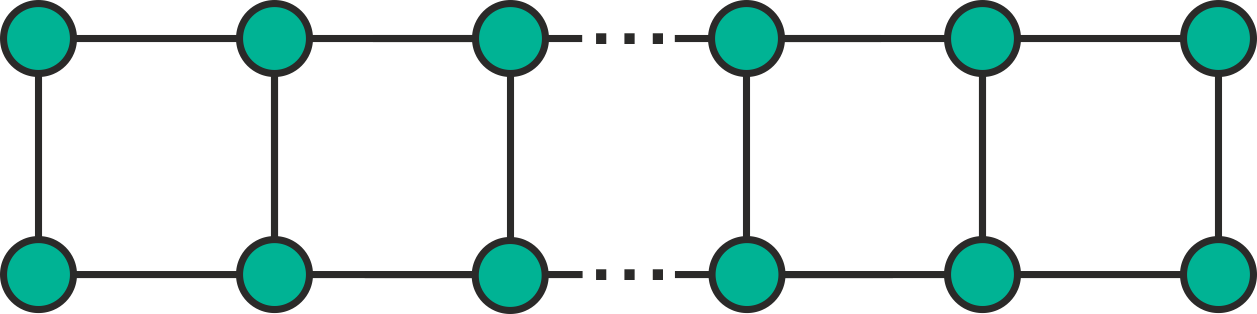
\includegraphics[width=30mm]{images/Fig_2_4_2.png}
    \vspace{-3ex}
\end{wrapfigure}
2C. Определите насколько отличается количество частот колебаний, разрешенных в ИК спектре, от количества частот колебаний, разрешенных в КР спектре, для плоской молекулы из $N$ одинаковых атомов, структура которой схематично изображена на рисунке.
\par
3С. Спектр комбинационного рассеяния карбонат-иона содержит 3 частоты. Используя данный спектр можно ли однозначно установить имеет ли карбонат-ион плоскую или объемную структуру?
\par
\begin{wrapfigure}{r}{58mm} %this figure will be at the right
    \centering
    \vspace{-1mm}
    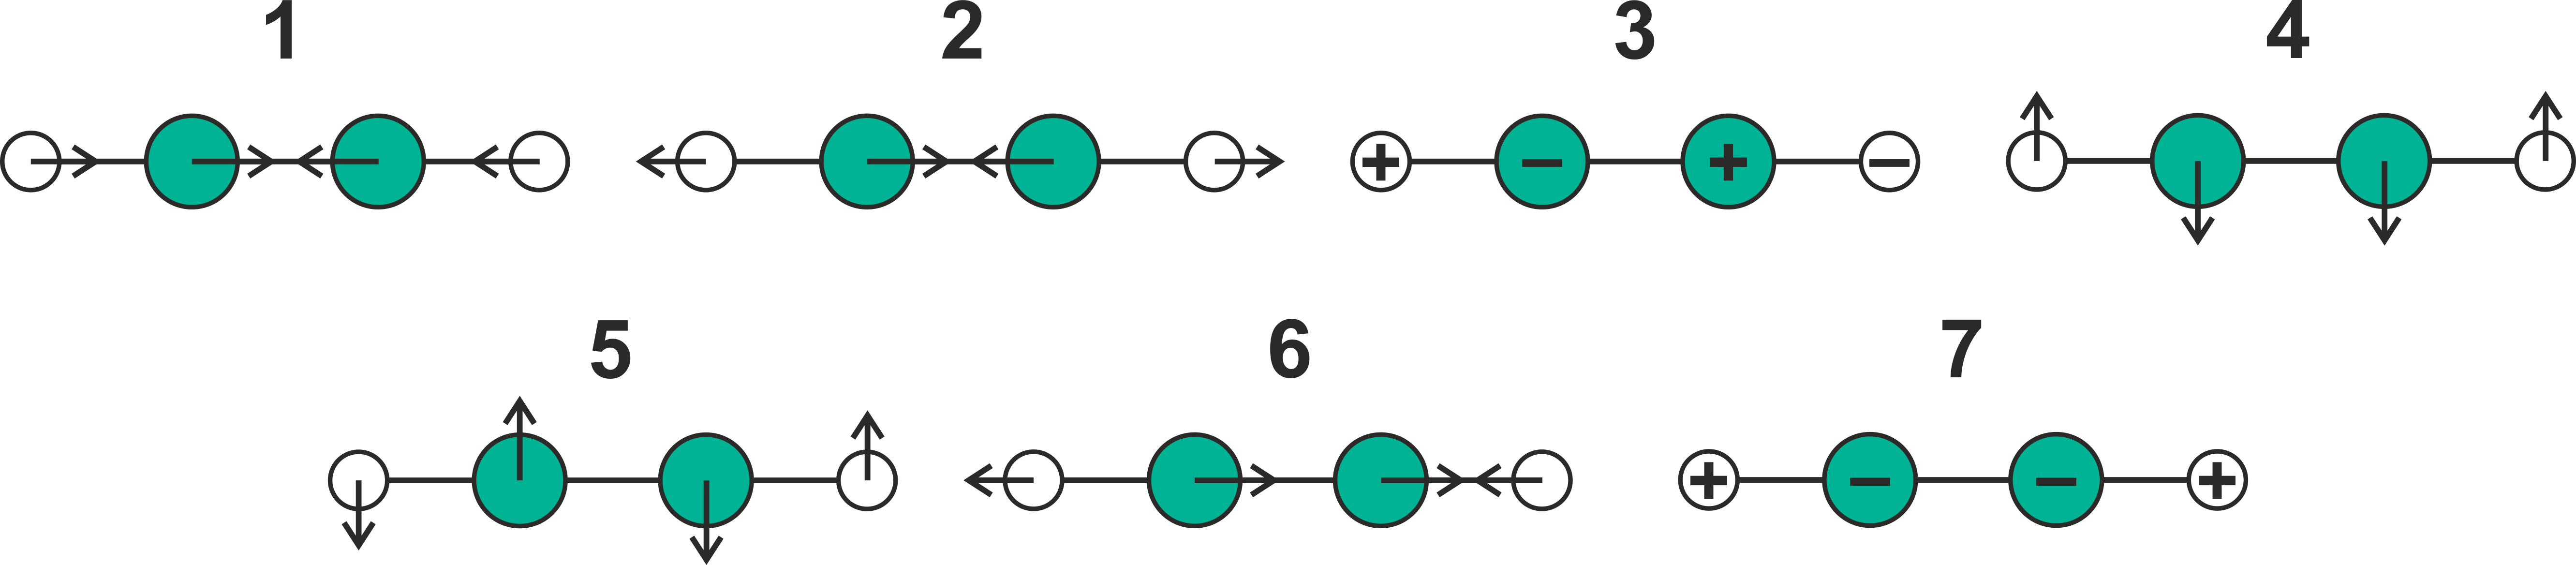
\includegraphics[width=58mm]{images/Fig_2_4_4.png}
    \vspace{-6mm}
\end{wrapfigure}
4К. Какие из изображенных на рисунке колебаний 1–7 молекулы ацетилена можно зарегистрировать с~помощью инфракрасной спектроскопии? Сколько им соответствует частот?
\par
5К. Определите симметрию колебаний цис-изомера плоской нелинейной молекулы $\text{N}_2\text{F}_2$. Какие колебания из найденных проявятся в спектре комбинационного рассеяния?
\par
\begin{wrapfigure}{r}{35mm} %this figure will be at the right
    \centering
    \vspace{-0.7ex}
    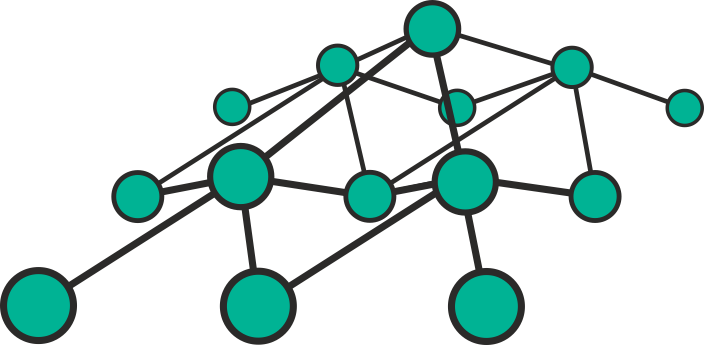
\includegraphics[width=28mm]{images/Fig_2_4_5.png}
    \vspace{-2ex}
\end{wrapfigure}
6C. Определите процент частот, наблюдаемых в ИК спектре, от общего числа частот для молекулы, имеющей строение четырехгранной пирамиды и состоящей из одинаковых атомов, уложенных плотноупакованными слоями как показано на рисунке. В~молекуле всего $N$ слоев, где $N$ – четное число.
\par
7. Какие изменения в количестве частот и их симметрии произойдут в ИК спектре сульфат-иона при его координации к атому металла через атом кислорода?
\par
8С. Можно ли с помощью ИК спектроскопии установить в какой конформации заслоненной или заторможенной находится молекула этана?
\par
9К. При исследовании методом инфракрасной спектроскопии некоторой пробы газообразного углекислого газа был получен спектр, в котором наблюдаются 4 частоты с волновыми числами: 667 и 649 см$^{-1}$, 2349 и 2283 см$^{-1}$. Соотношение интенсивностей в каждой из двух групп линий равно 100 к 1. Определите количество частот, которые должны наблюдаться в ИК спектре углекислого газа, а~также их симметрию. Объясните природу описанного выше экспериментального спектра, в частности природу указанных двух групп линий и относительного положения линий внутри каждой группы. Как будет выглядеть спектр комбинационного рассеяния данной пробы?
\par
10К. Определите число и симметрию валентных и деформационных колебаний в молекуле метана.
\par
11К. Можно ли с помощью ИК спектроскопии различить цис- и транс- изомеры октаэдрического комплекса $[\text{FeCl}_4\text{Br}_2]^{3-}$. 
\par
\setmainfont{Noto Serif}
\setsansfont{Noto Sans}
\setmonofont{Noto Sans Mono}
\setstretch{1.35}

\section{Эффект Яна-Теллера}
1С. Используя теорию поля лигандов определите в каких из тетрахлорных комплексов $\text{[MeCl}_4]^{2-}$ кобальта, никеля и меди проявляется эффект Яна-Теллера. Для ян-теллеровских комплексов определите симметрию колебания, которое приводит к понижению симметрии.
\par
2С. В каких циклических системах возможен линейный эффект Яна-Теллера? Для случая циклопропиенильного радикала установите симметрию колебания, которое приводит к искажению геометрии. Определите также изменение полной электронной энергии данного радикала при понижении симметрии с $D_{3h}$ до $C_{2v}$. Считайте, что резонансные интегралы соответствующих связей изменились на 10\%.
\par
3. Определите проявляется ли эффект Яна-Теллера в молекулах $\text{BeH}_2$, $\text{CO}$.
\par
\begin{wrapfigure}{r}{25mm} %this figure will be at the right
    \centering
    \vspace{-2.6ex}
    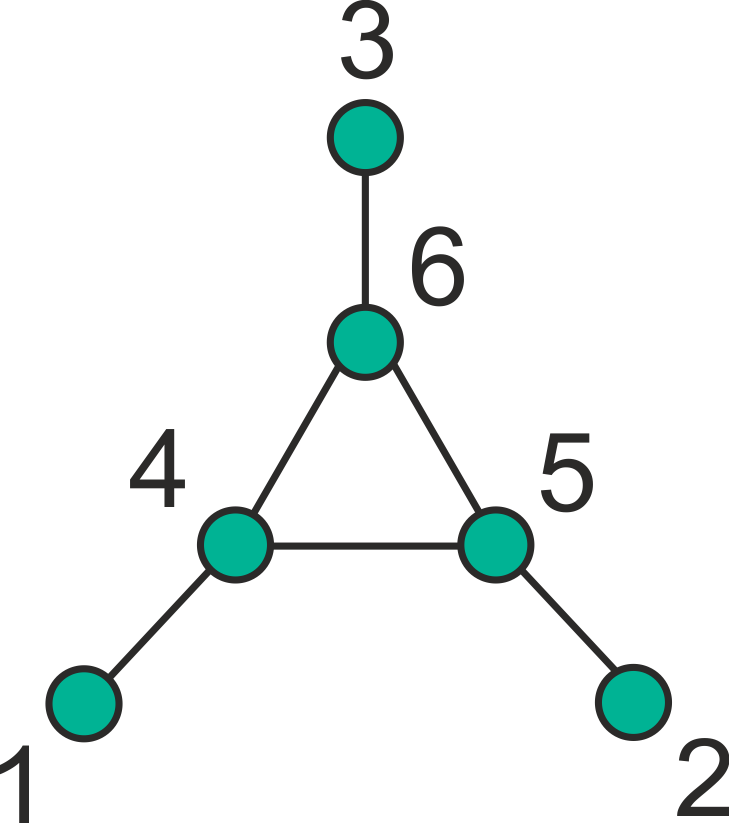
\includegraphics[width=16.5mm]{images/Fig_2_5_4.png}
    \vspace{-5ex}
\end{wrapfigure}
4С. Для какой формы (нейтральная молекула, катион-, анион-радикал) хюккелевской системы, изображенной на~рисунке может быть характерен эффект Яна-Теллера?
\par
5. Какова геометрия иона $\text{CH}_4^+$?
\par
6. Рассмотреть стабильность октаэдрических комплексов металлов с конфигурацией $d^1$–\,$d^{10}$ в высокоспиновом состоянии по отношению к эффекту Яна-Теллера.
\par
\begin{wrapfigure}{r}{45mm} %this figure will be at the right
    \centering
    \vspace{-4mm}
    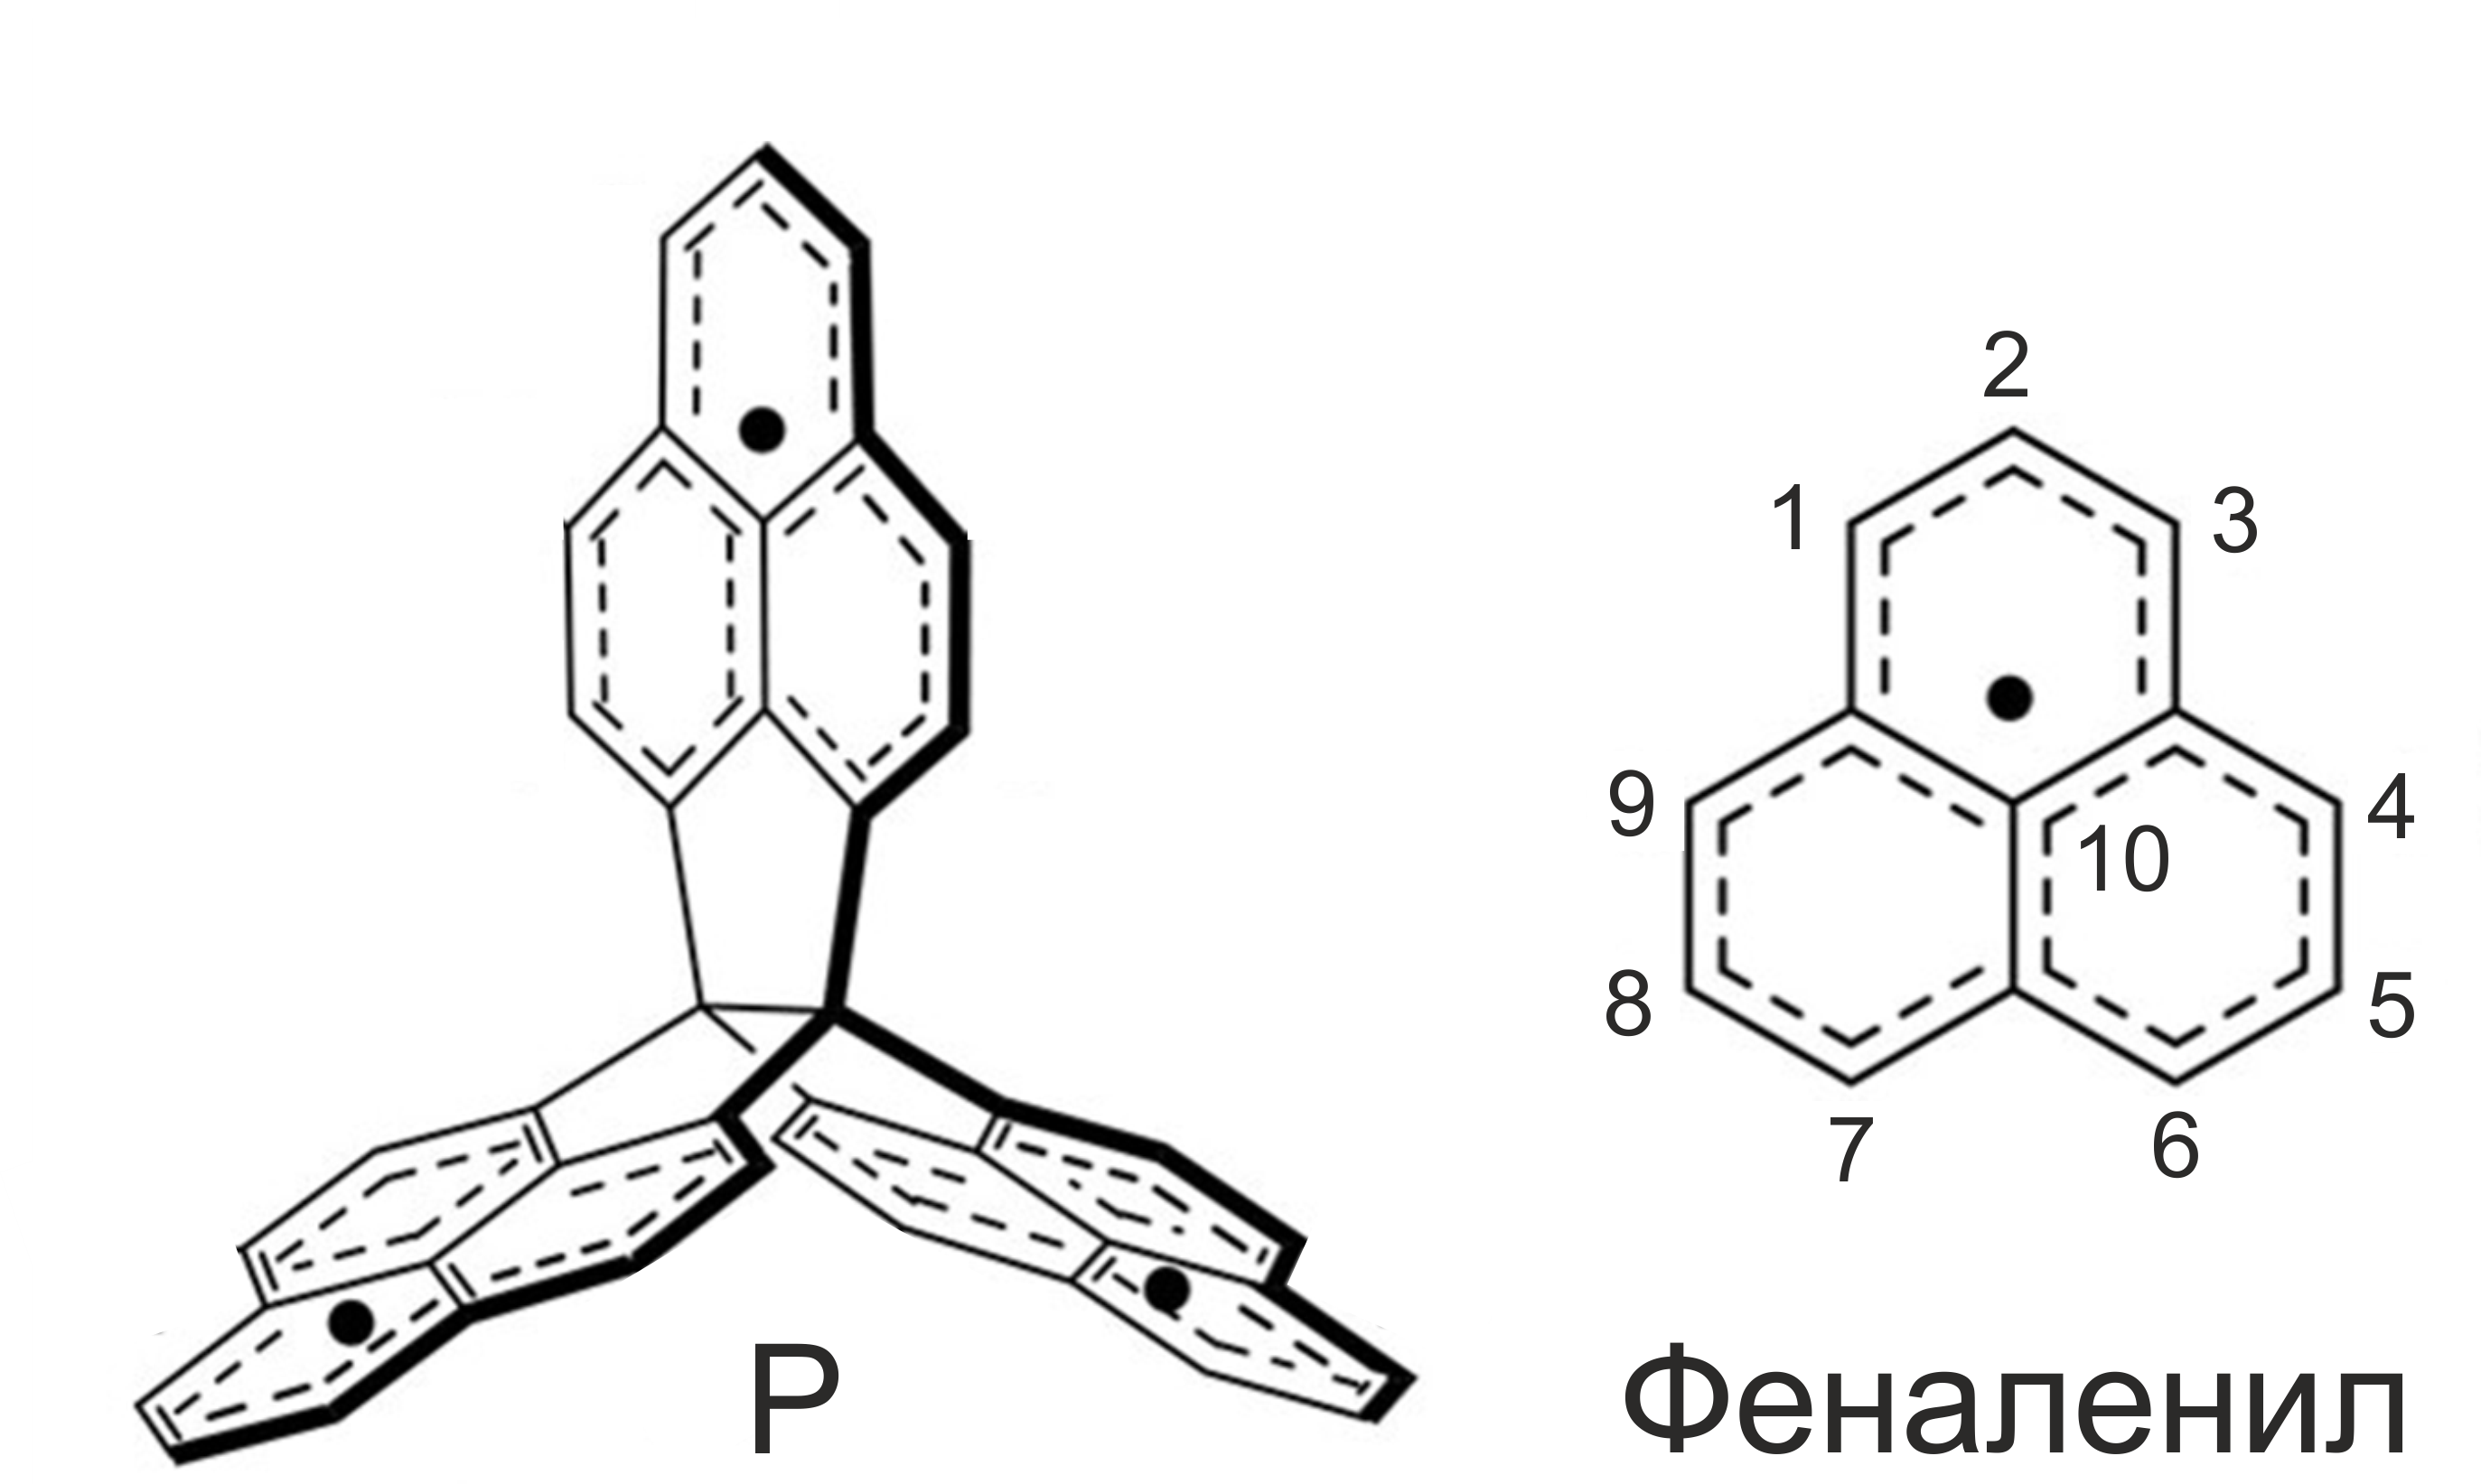
\includegraphics[width=45mm]{images/Fig_2_5_7.png}
    \vspace{-6mm}
\end{wrapfigure}
7К. В 2022 году японскими химиками был синтезирован пропеллероподобный трирадикал P на основе трех молекул феналенила. Структурные формулы P и феналенила приведены на рисунке справа. Используя однократно занятые молекулярные орбитали феналенила, определите вид и симметрию граничных молекулярных орбиталей трирадикала P, а также его основной терм. Подвержен ли P эффекту Яна-Теллера?
\par
8. Определите типы колебаний молекулы бензола, ответственные за такое перераспределение интенсивностей в его спектре поглощения, при котором за~счет разрешенного электронного перехода $A_{1g}$ $\rightarrow$ $E_{1u}$ возникают спектральные переходы $A_{1g}$ $\rightarrow$ $B_{1u}$ и $A_{1g}$ $\rightarrow$ $B_{2u}$.
\par
9. Показать, что для эффекта Яна-Теллера второго порядка существенны только колебания, симметрия которых совпадает с симметрией нижнего возбужденного состояния.
\par

\setmainfont{Noto Serif}
\setsansfont{Noto Sans}
\setmonofont{Noto Sans Mono}
\setstretch{1.35}

\section{Вращательная спектроскопия и ее производные}
1С. Для двухатомной молекулы XY в состоянии с колебательным квантовым числом $\nu$ = 1 межъядерное расстояние увеличено на 1\% по сравнению с расстоянием для $\nu$ = 0. Какая линия R-ветви в колебательно-вращательном спектре будет соответствовать максимальной энергии (предел канта).
\par
2С. Вращательные переходы $J + 1$ $\leftarrow$ $J$ в двух линейных изотопологах $^{16}\text{O}^{12}\text{C}^{32}\text{S}$ и~$^{16}\text{O}^{12}\text{C}^{34}\text{S}$ соответствуют частотам, приведенным в~единицах ГГц для некоторых $J$ в таблице ниже.
\begin{center}
\begin{tabular}{ c c c c c }

 J & 1 & 2 & 3 & 4 \\ 
 \hline
 $^{16}$O$^{12}$C$^{32}$S & 24,32592 & 36,48882 & 48,65164 & 60,81408 \\  
 $^{16}$O$^{12}$C$^{34}$S & 23,73223 & $-$ & 47,4620 & $-$    
\end{tabular}
\end{center}
Определите величину вращательной постоянной и момент инерции для изотополога $^{16}\text{O}^{12}\text{C}^{32}\text{S}$, а также длины связей $\text{O}-\text{C}$ и $\text{S}-\text{C}$, считая что для данных изотопологов оно одинаковое.
\par
3С. Вращательная постоянная молекулы $^1$H$^{35}$Cl равна 10,4400 см$^{-1}$ для основного колебательного состояния и 10,1366 см$^{-1}$ для первого возбужденного. Нарисуйте вращательно-колебательный спектр данной молекулы в окрестности фундаментальной частоты 2990,95 см$^{-1}$.
\par
4С. Покажите, что вращательные энергетические уровни плоской квадратной молекулы XY$_4$ могут быть выражены используя только вращательную постоянную $B$.
\par
5. Трехатомная молекула имеет строение X$_2$Y. Ее вращательный спектр имеет линии поглощения с частотой 20 ГГц, 40 ГГц, 60 ГГц и т.д. Какая из следующих структур соответствует данной молекуле: X$-$X$-$Y (линейная), X$-$Y$-$X (линейная), X$-$Y$-$X (изогнутая), X$-$X$-$Y (изогнутая)?
\par
6С. Классифицируйте ядерные спиновые изомеры линейной молекулы $\text{BeH}_2$. Ядерный спин единственного природного изотопа равен $I$($^9\text{Be}$) = 3/2.
\par
7С. Постройте вращательно-колебательной спектр молекулы углекислого газа.
\par
8С. Постройте вращательно-колебательный спектр молекулы ацетилена, считая что ее основной терм $^1\Sigma^+_g$. Какие изменения произойдут в спектре если все углеродные атомы $^{12}\text{C}$ заменить на $^{13}\text{C}$?
\par
9С. Определите процент линейных молекул $\text{Cl}-\text{O}-\text{Cl}$, имеющих только четные вращательные уровни. $I$($^{35}\text{Cl}$) = $I$($^{37}\text{Cl}$) = 3/2. Считайте, что природное содержание изотопа $^{35}\text{Cl}$ в три раза больше, чем содержание изотопа $^{37}\text{Cl}$.
\par
10. При каком ядерном спине в чисто вращательном спектре комбинационного рассеяния двухатомной гомоядерной молекулы интенсивность первой и~второй линии будет одинакова?
\par
11К. В лаборатории физиологии фантастических тварей проводились исследования источника топлива огненного дыхания Змея Горыныча. Физико-хими-ческий анализ несгораемых остатков показал, что топливо представляет собой двухатомную молекулу T с приведенной массой 1,615$\cdot$10$^{-27}$ кг. Микроволновый спектр соединения T содержит набор эквидистантных линий с расстоянием между линиями 22,04 см$^{-1}$. Используя приближение жесткого ротора определите длину связи в молекуле T. Что это может быть за молекула? Примечание: 1 а. е. м. = 1,6605$\cdot$10$^{-27}$ кг, $\hbar$ = 1,05$\cdot$10$^{-34}$ Дж$\cdot$с.
\par
12К. Из термодинамических соображений следует, что моногалогениды меди CuX должны существовать в газовой фазе в основном в виде полимеров, что подтверждается экспериментально. Эта проблема может быть решена путем пропускания газообразного галогена над медью, нагретой до 1100 К. Так, в~газообразном $^{63}\text{Cu}^{81}\text{Br}$ были зарегистрированы переходы между вращательными уровнями с квантовыми числами 13 $\rightarrow$ 14, 14 $\rightarrow$ 15 и 15 $\rightarrow$ 16 на частотах 84421,34; 90449,25 и 96476,72 МГц, соответственно. Определите вращательную постоянную и длину связи для $^{63}\text{Cu}^{81}\text{Br}$. Примечание: 1 а. е. м. = 1,6605$\cdot$10$^{-27}$ кг, $\hbar$ = 1,05$\cdot$10$^{-34}$ Дж$\cdot$с.
\par
13К. Квадрат электрического дипольного момента перехода между двумя вращательными уровнями зависит от вращательного квантового числа $J$ следующим образом: $|d_{J+1,\,J}|^2 \sim \frac{J+1}{2J+1}$. Предскажите вид чисто вращательного спектра молекулы $^{1}\text{H}^{35}\text{Cl}$ при температуре 300 К без учета и с учетом приведенного фактора. В частности, в каждом случае определите значение $J$, соответствующее линии поглощения с наибольшей относительной интенсивностью. Вращательная постоянная $^{1}\text{H}^{35}\text{Cl}$ равна 10,6 см$^{-1}$.
\par
\setmainfont{Noto Serif}
\setsansfont{Noto Sans}
\setmonofont{Noto Sans Mono}
\setstretch{1.35}

\section{ЭПР спектроскопия}
1С. Постройте спектр ЭПР катион-радикала дурола.
\par
\begin{wrapfigure}{r}{20mm} %this figure will be at the right
   \centering
    \vspace{-3.6ex}
    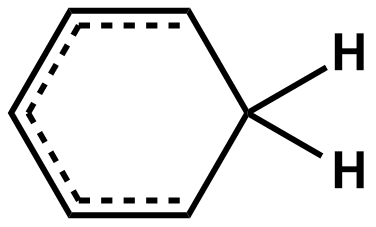
\includegraphics[width=15mm]{images/Fig_2_7_1.png}
    \vspace{-4ex}
\end{wrapfigure}
2С. Постройте спектр ЭПР радикала, структура которого изображена на рисунке. Константа СТВ с $\beta$-протонами в данном радикале равна 4,5~мТл.
\par
3К. Определите процентное содержание изотопа $^{13}\text{C}$ в метильном радикале, если соотношение интенсивностей трех высокопольных линий в спектре ЭПР данного радикала равно 1:3:3, начиная с самой высокопольной. Константа СТВ с ядром $^{13}\text{C}$ равна 40 Гс.
\par
4С. Постройте спектр ЭПР для радикала $\text{NH}_2^{\boldsymbol{\cdot}}$. Константы сверхтонкого взаимодействия равны: $a_{\text{N}}$ = 10 Гс, $a_{\text{H}}$ = 24 Гс. Как изменится спектр, если один атом водорода заменить на дейтерий?
\par
5С. Какая температура необходима, чтобы ориентировать 75\% спинов некоторого радикала в магнитном поле 1 Тл?
\par
6С. Нарисуйте спектр ЭПР во втором порядке теории возмущений для следующих радикалов: $\text{H}$, $\text{H}_2^{\boldsymbol{\cdot}}$, $\text{D}$, $^{\boldsymbol{\cdot}}\text{CH}_3$.
\par
7С. Нарисуйте спектр ЭПР $\text{D}_2^{+\boldsymbol{\cdot}}$ при $T \rightarrow$ 0 К.
\par
8. В рамках теории возмущений второго порядка рассчитайте как будет выглядеть спектр ЭПР иона ванадила, если $a$ = 100 Гс, $g$ = 2, $I$ = 7/2, $\nu$ = 9000 МГц.
\par
9К. Метильный радикал стабилизировали в некоторой дейтерированной матрице. С течением времени произошел обмен атомов водорода радикала и~дейтерия матрицы. Постройте ЭПР спектр эквимолярной смеси $^{\boldsymbol{\cdot}}\text{CHD}_2$ и $^{\boldsymbol{\cdot}}\text{CH}_2\text{D}$ радикалов. Укажите, сравнивая относительные интенсивности каких линий, возможно определить содержание данных радикалов в смеси.
\par
\begin{wrapfigure}{r}{20mm} %this figure will be at the right
   \centering
    \vspace{0.55ex}
    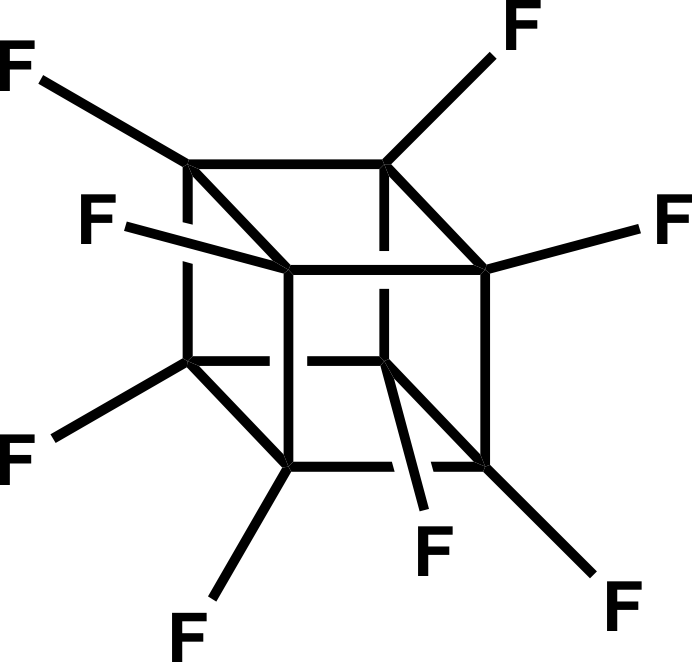
\includegraphics[width=20mm]{images/Fig_2_7_10.png}
    \vspace{-3ex}
\end{wrapfigure}
10К. Фторированные аналоги полиэдрических углеводородов локализуют электрон внутри полости своего каркаса при их восстановлении. В 2022 году японским химикам удалось синтезировать перфторкубан и стабилизировать его анион-радикал, полученный в результате $\gamma$-облучения, в матрице гексаметилэтана при 77 К. Нарисуйте спектр ЭПР данного анион-радикала с учетом второго порядка теории возмущений. Считайте, что неспаренный электрон локализован в каркасе перфторкубана, а константа СТВ на ядрах фтора равна 196,2 Гс.
\par
\begin{wrapfigure}{r}{25mm} %this figure will be at the right
   \centering
    \vspace{-4ex}
    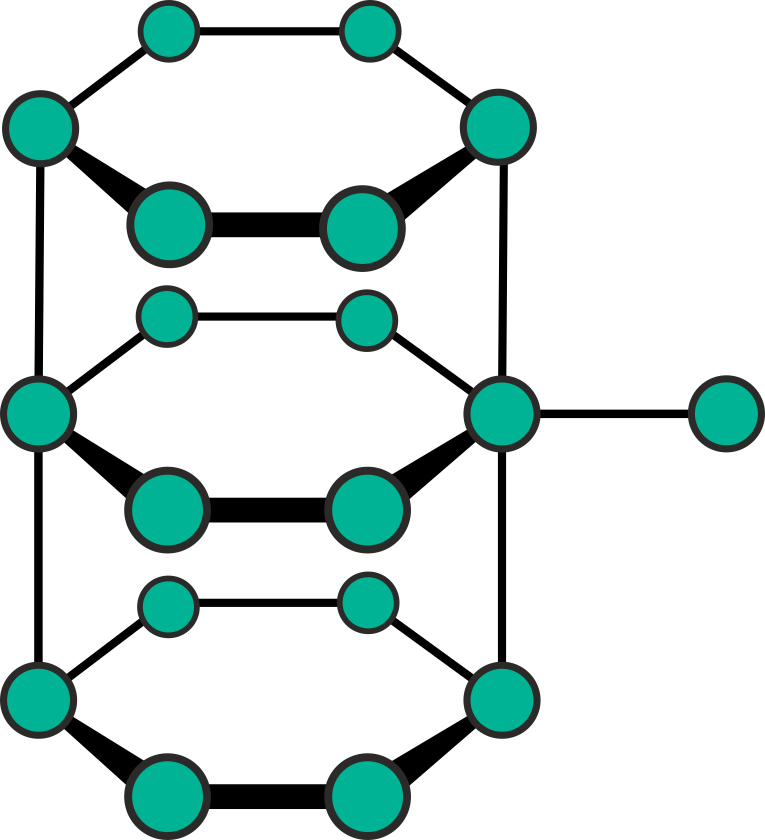
\includegraphics[width=14mm]{images/Fig_2_7_12.png}
    \vspace{-4ex}
\end{wrapfigure}
11C. Для хюккелевской системы, структура которой изображена на рисунке, постройте спектр ЭПР. Определите количество линий в~этом спектре и их относительную интенсивность.
\par
12С. Постройте спектр ЭПР для радикала $\text{H}_2^{+ \boldsymbol{\cdot}}$ в нулевом внешнем магнитном поле и $T$ $\rightarrow$ 0 К.
\par
13С. Построить спектры ЭПР радикала $\text{CF}_3$ с константой СТВ $a_{\text{F}}$ = 142 Гс и радикала $^{13}\text{CF}_3$ с константами СТВ $a_{\text{F}}$ = 142 Гс, $a_{^{13}\text{C}}$ = 272 Гс с учетом второго порядка теории возмущений.
\par

\setmainfont{Noto Serif}
\setsansfont{Noto Sans}
\setmonofont{Noto Sans Mono}
\setstretch{1.35}

\section{Химический обмен в магнитном резонансе}
1C. Изобразите трансформацию спектра ЭПР при увеличении скорости химической реакции: 
\text{H} + $\text{H}_2$ $\rightleftarrows$ $\text{H}_3$ (циклическая система).
\par
\begin{wrapfigure}{r}{51mm} %this figure will be at the right
    \centering
    \vspace{-0mm}
    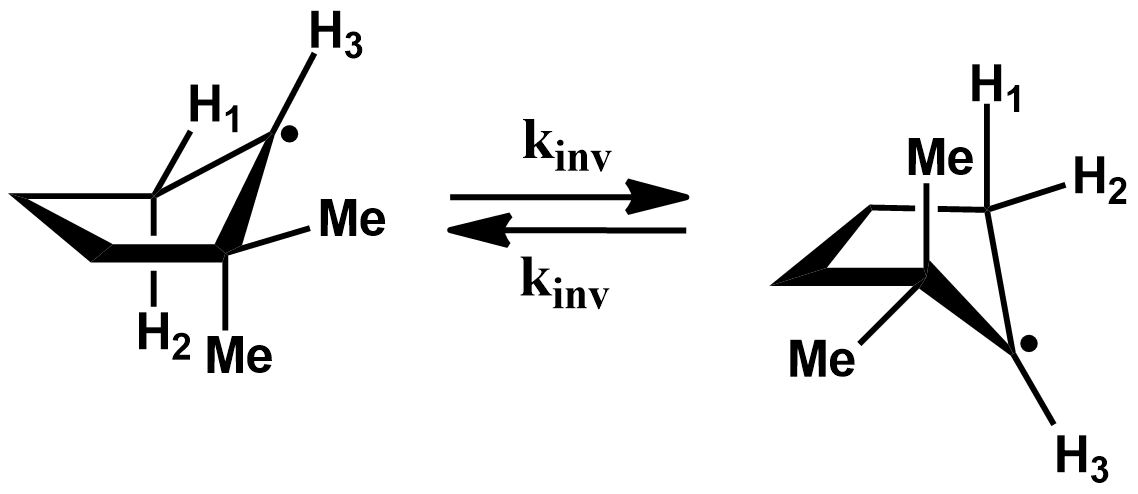
\includegraphics[width=45mm]{images/Fig_2_8_2.png}
    \vspace{-4mm}
\end{wrapfigure}
2К. 2,2-диметилциклопентильный радикал имеет две инверсные конформации, приведенные на рисунке. Константа СТВ протона в третьем положении равна 15~Гс, а протонов $\text{CH}_2$-фрагмента 20 Гс и 10~Гс в~экваториальном и аксиальном положениях, соответственно. Постройте спектр ЭПР данного радикала для случаев: (1)~отсутствия обмена экваториальных и аксиальных протонов $\text{H}_1$ $\rightleftarrows$ $\text{H}_2$, (2)~медленного обмена при $k_{inv}$ $\ll$ СТВ, (3)~быстрого обмена при $k_{inv}$ $\gg$ СТВ.
\par
\begin{wrapfigure}{r}{51mm} %this figure will be at the right
    \centering
    \vspace{-0mm}
    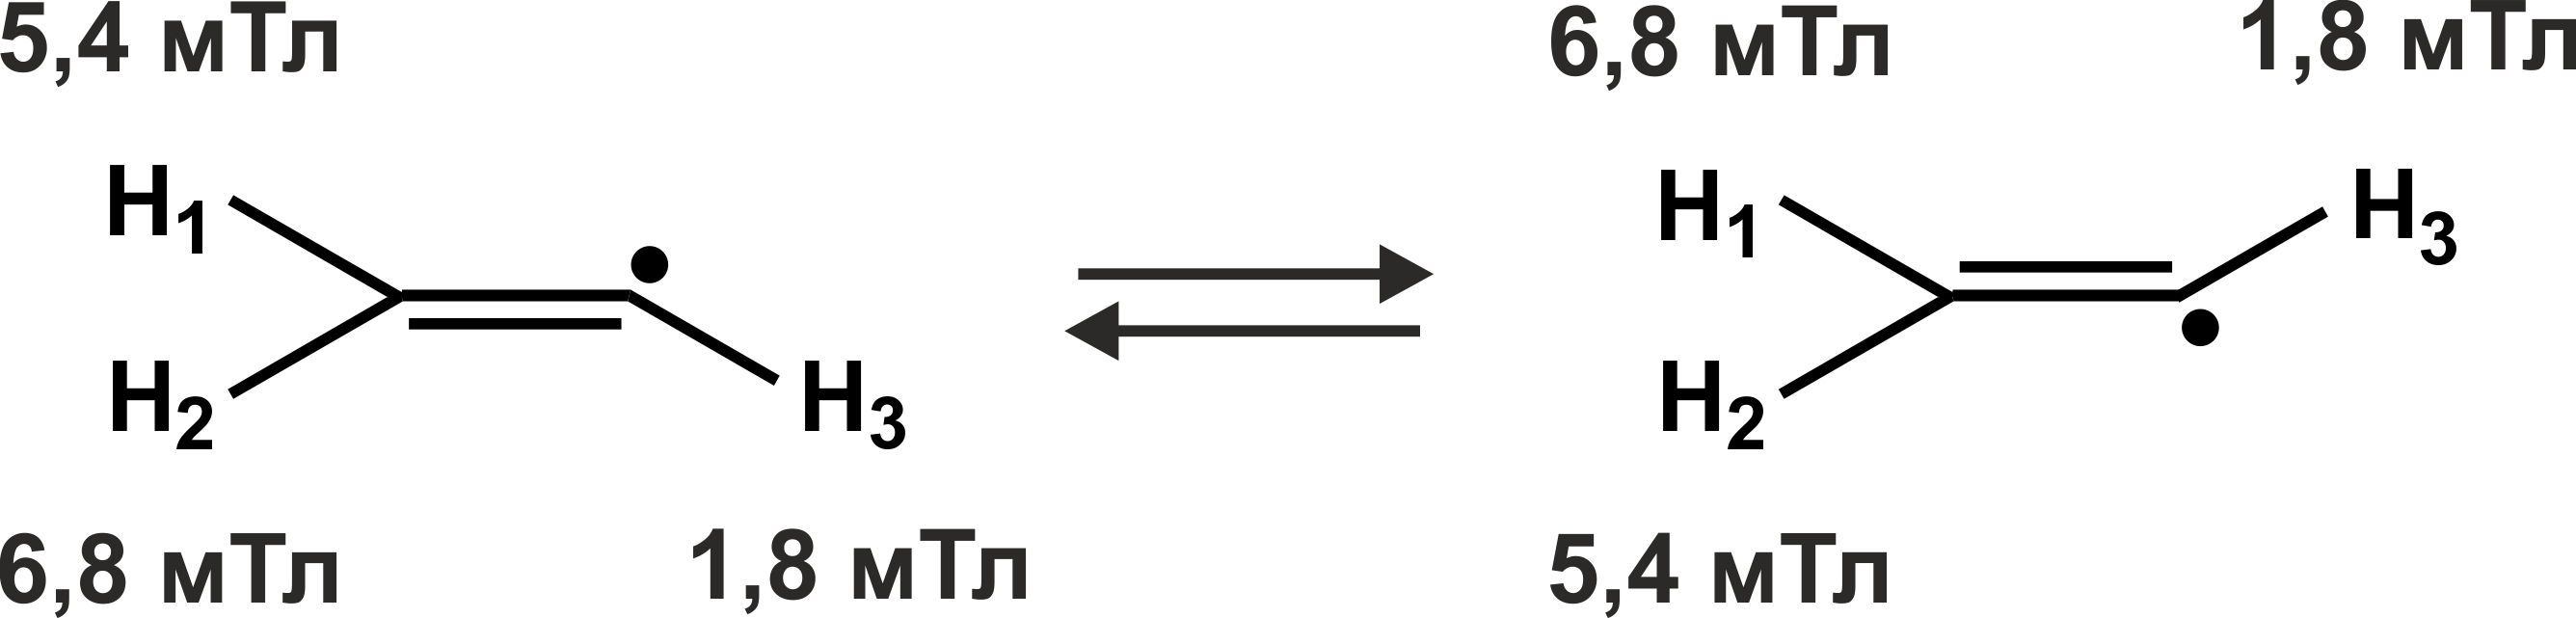
\includegraphics[width=51mm]{images/Fig_2_8_4.png}
    \vspace{-4mm}
\end{wrapfigure}
3К. Опишите изменения в спектре ЭПР винильного радикала, происходящие при увеличении скорости превращения его таутомеров. Константы СТВ приведены на рисунке справа. В частности нарисуйте ЭПР спектр, наблюдаемый при низкой температуре в жесткой матрице, спектр, наблюдаемый при промежуточной температуре, а также ЭПР спектр, регистрируемый в невязкой жидкости.
\par
4С. В кристаллах алмаза наблюдаются дефекты с одним неспаренным электроном, содержащие азот следующего типа: $\text{N}_1-\text{C}-\text{N}_2$. Неспаренный электрон взаимодействует с ядрами азота, имеющими константу $a_1$ = 30 Гс и $a_2$ = 5 Гс, соответственно. Причем $a_1$ и $a_2$ могут иметь одинаковые знаки и различные знаки, могут быть как положительными, так и отрицательными. При повышении температуры происходит обмен ядрами азота: $\text{N}_1-\text{C}-\text{N}_2$ $\rightleftarrows$ $\text{N}_2-\text{C}-\text{N}_1$. Опишите картину процесса в двух случаях, различающихся знаками одной из~констант СТВ: (1) $a_1$ = 30 Гс и $a_2$ = +5 Гс, (2) $a_1$ = 30 Гс и $a_2$ = $-$5 Гс.
\par
5С. Определите изменение спектров ЯМР, полученных на ядрах $^{19}\text{F}$ и $^{31}\text{P}$, для молекулы $\text{PF}_5$ при увеличении скорости: (1) внутримолекулярного обмена всех атомов фтора, (2) межмолекулярного обмена аксиальных атомов фтора. Константы спин-спинового взаимодействия уменьшаются в следующем порядке: $J(\text{P}-\text{F}_\text{a})$ $>$ $J(\text{P}-\text{F}_\text{э})$ $>$ $J(\text{F}_\text{э}-\text{F}_\text{a})$.
\par
\begin{wrapfigure}{r}{33mm} %this figure will be at the right
    \centering
    \vspace{0.7mm}
    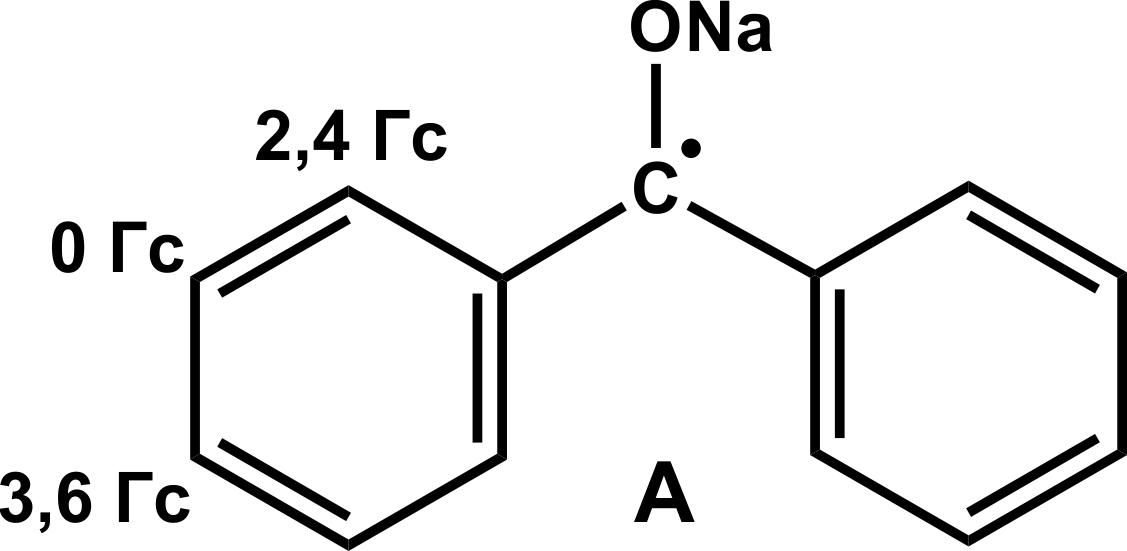
\includegraphics[width=33mm]{images/Fig_2_8_8.png}
    \vspace{0mm}
\end{wrapfigure}
6К. ЭПР спектр разбавленного раствора кетила бензофенона натрия, соединение А, в 1,2-диметок-сиэтане содержит 52 линии. Константы СТВ в анион-радикале бензофенона приведены на рисунке. Объясните, чем может быть вызвано такое количество линий в спектре ЭПР данного кетила. В присутствии избытка бензофенона в растворе также протекает реакция:
\[\text{NaO}\boldsymbol{\dot{\text{C}}}(\text{C}_6\text{H}_5)_2 + \text{O}\text{C}(\text{C}_6\text{H}_5)_2 = \text{O}\text{C}(\text{C}_6\text{H}_5)_2 + \text{NaO}\boldsymbol{\dot{\text{C}}}(\text{C}_6\text{H}_5)_2\]
С помощью ЭПР спектроскопии возможно установить протекает ли данная реакция (1) в результате переноса атома натрия или (2) в результате некоррелированного переноса электронов и катионов натрия $\text{Na}^+$. Как будет выглядеть спектр ЭПР смеси при достаточной высокой для протекания быстрого обмена концентрации бензофенона в указанных двух случаях. Кетилами называют анион-радикалы общей формулы $\text{R}_2 \boldsymbol{\dot{\text{C}}}-\text{O}^-$ и их соли, то есть продукты одноэлектронного восстановления кетонов.
\par
\setmainfont{Noto Serif}
\setsansfont{Noto Sans}
\setmonofont{Noto Sans Mono}
\setstretch{1.35}

\section{ЯМР спектроскопия}
1С. Нарисуйте спектры $^1\text{H}$, $^{13}\text{C}$ и $^{19}\text{F}$ ЯМР следующих соединений: (1) $\text{CH}_3\text{CH}_2\text{OH}$, (2) $\text{CH}_3\text{CH}\text{O}$, (3) $\text{CH}_3\text{CH}_2\text{O}\text{CH}_3$, (4) $\text{CF}_3\text{H}$.
\par
2С. В спектре $^1\text{H}$ ЯМР соединения $\text{C}_{6}\text{H}_{6}\text{N}_{6}\text{O}_{6}$ присутствует одна линия с химическим сдвигом 10,2 м. д. В спектре $^{13}\text{C}$ ЯМР присутствует две линии. Определите структуру молекулы.
\par
3С. Определите структуры соединений по приведенным ниже $^1\text{H}$ ЯМР спектрам и брутто-формулам: (1) $\text{C}_{9}\text{H}_{13}\text{N}$, (2) $\text{C}_{3}\text{H}_{4}\text{F}_4\text{O}$.
\begin{figure}[h]
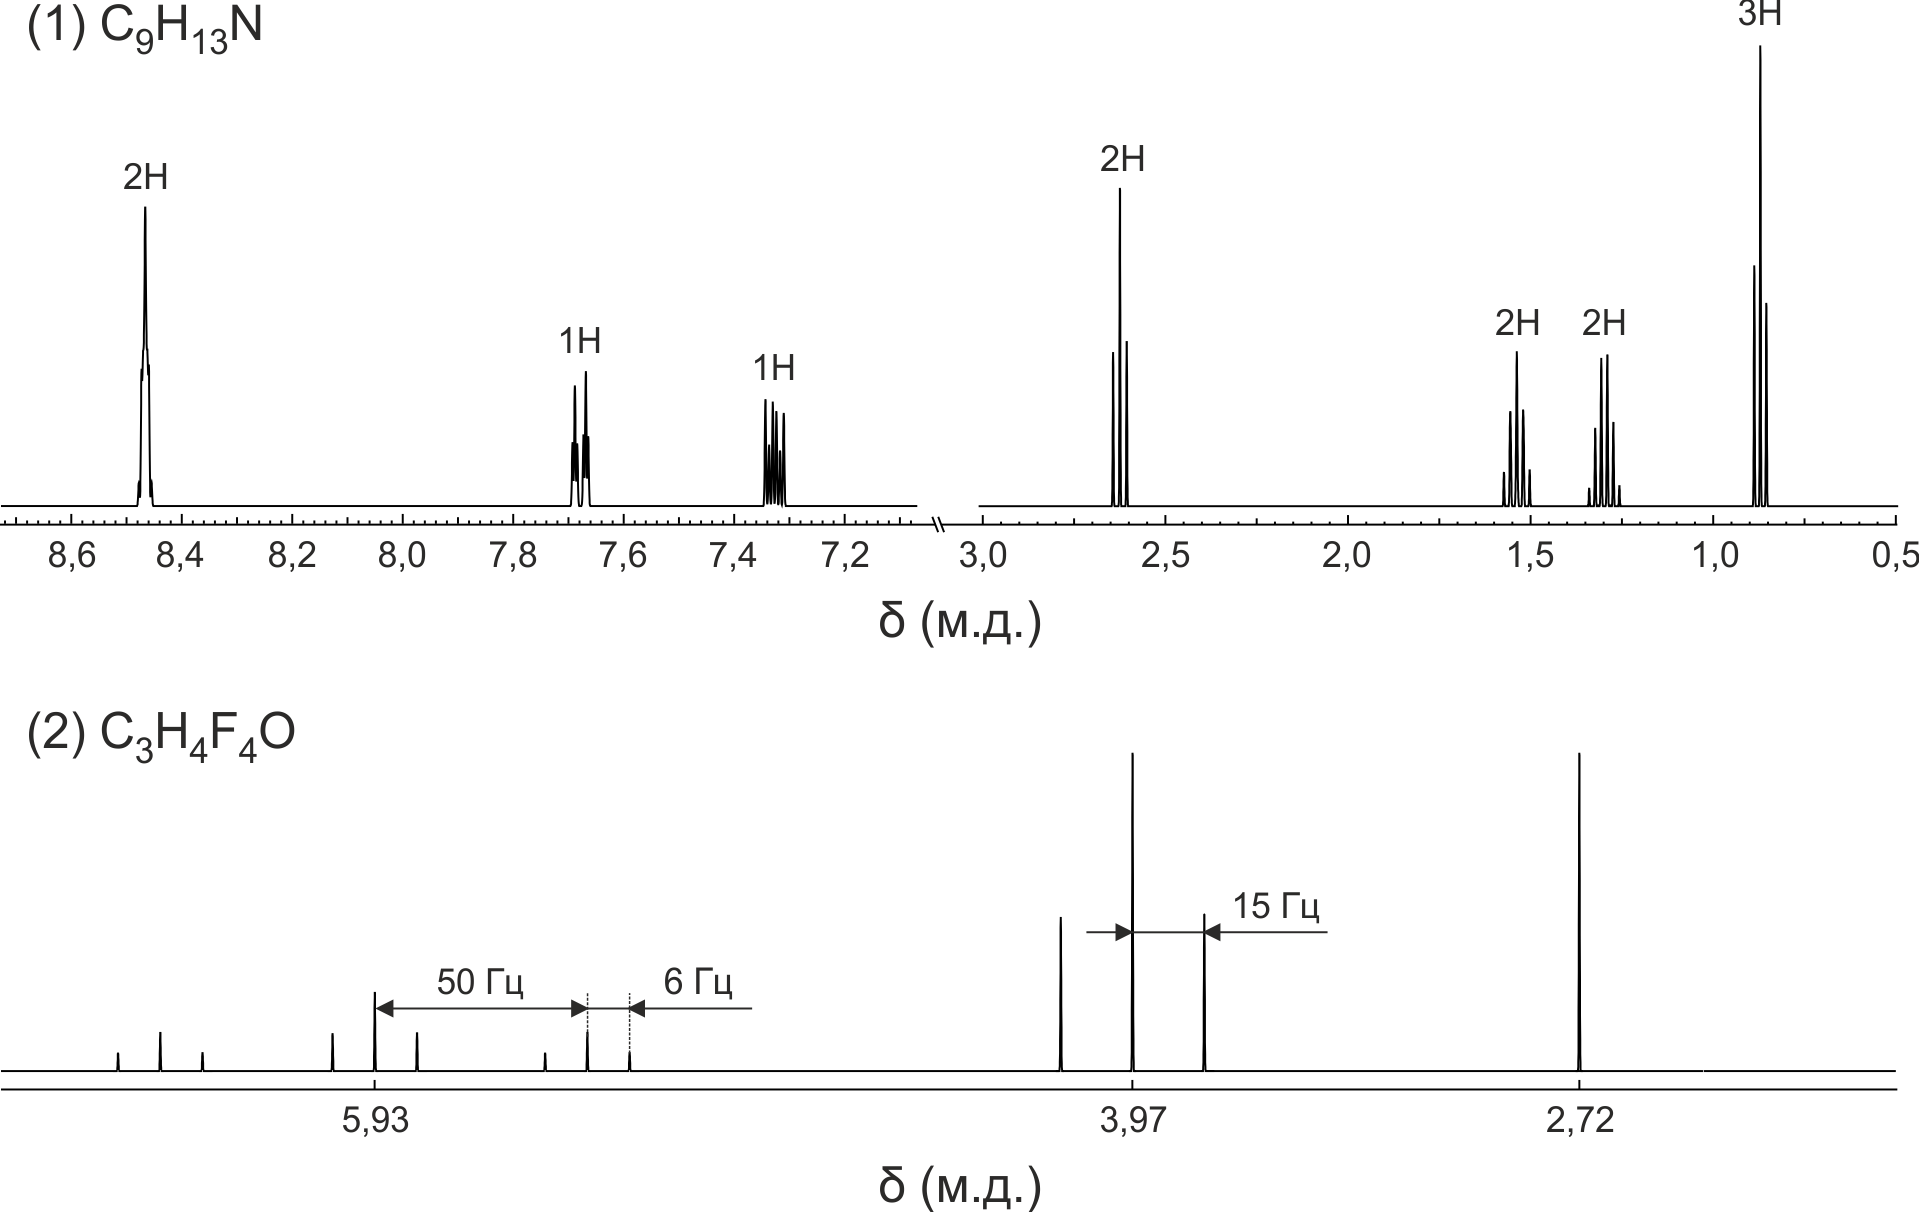
\includegraphics[width=10cm]{images/Fig_2_9_3.png}
\centering
\end{figure}
\par
\vspace{-\parskip}
4С. Определите структуры соединений по приведенным описаниям $^1\text{H}$ ЯМР спектров и брутто-формулам:\\ 
(1) $\text{C}_{3}\text{H}_{6}\text{O}$: $^1$H ЯМР (400 МГц) $\delta$ (м. д.): 5,0 (т, 4H); 2,0~(квинт, 2H);\\
(2) $\text{C}_{5}\text{H}_{11}\text{Cl}$: $^1$H ЯМР (400 МГц) $\delta$ (м. д.): 3,57 (т, 2H, $J$ = 6,8 Гц); 1,72 (дт, 2H, $J$ = 7,2; 6,8~Гц); 1,46 (м, 1H, $J$ = 6,6; 7,2 Гц); 0,88 (д, 6H, $J$ = 6,6 Гц);\\
(3) $\text{C}_{6}\text{H}_{9}\text{Br}\text{O}_{3}$: $^1$H ЯМР (400 МГц) $\delta$ (м. д.): 3,66 (c, 3H); 2,53 (c, 3H); 1,86 (c, 3H).
\par
\begin{wrapfigure}{r}{37mm} %this figure will be at the right
    \centering
    \vspace{-3.2mm}
    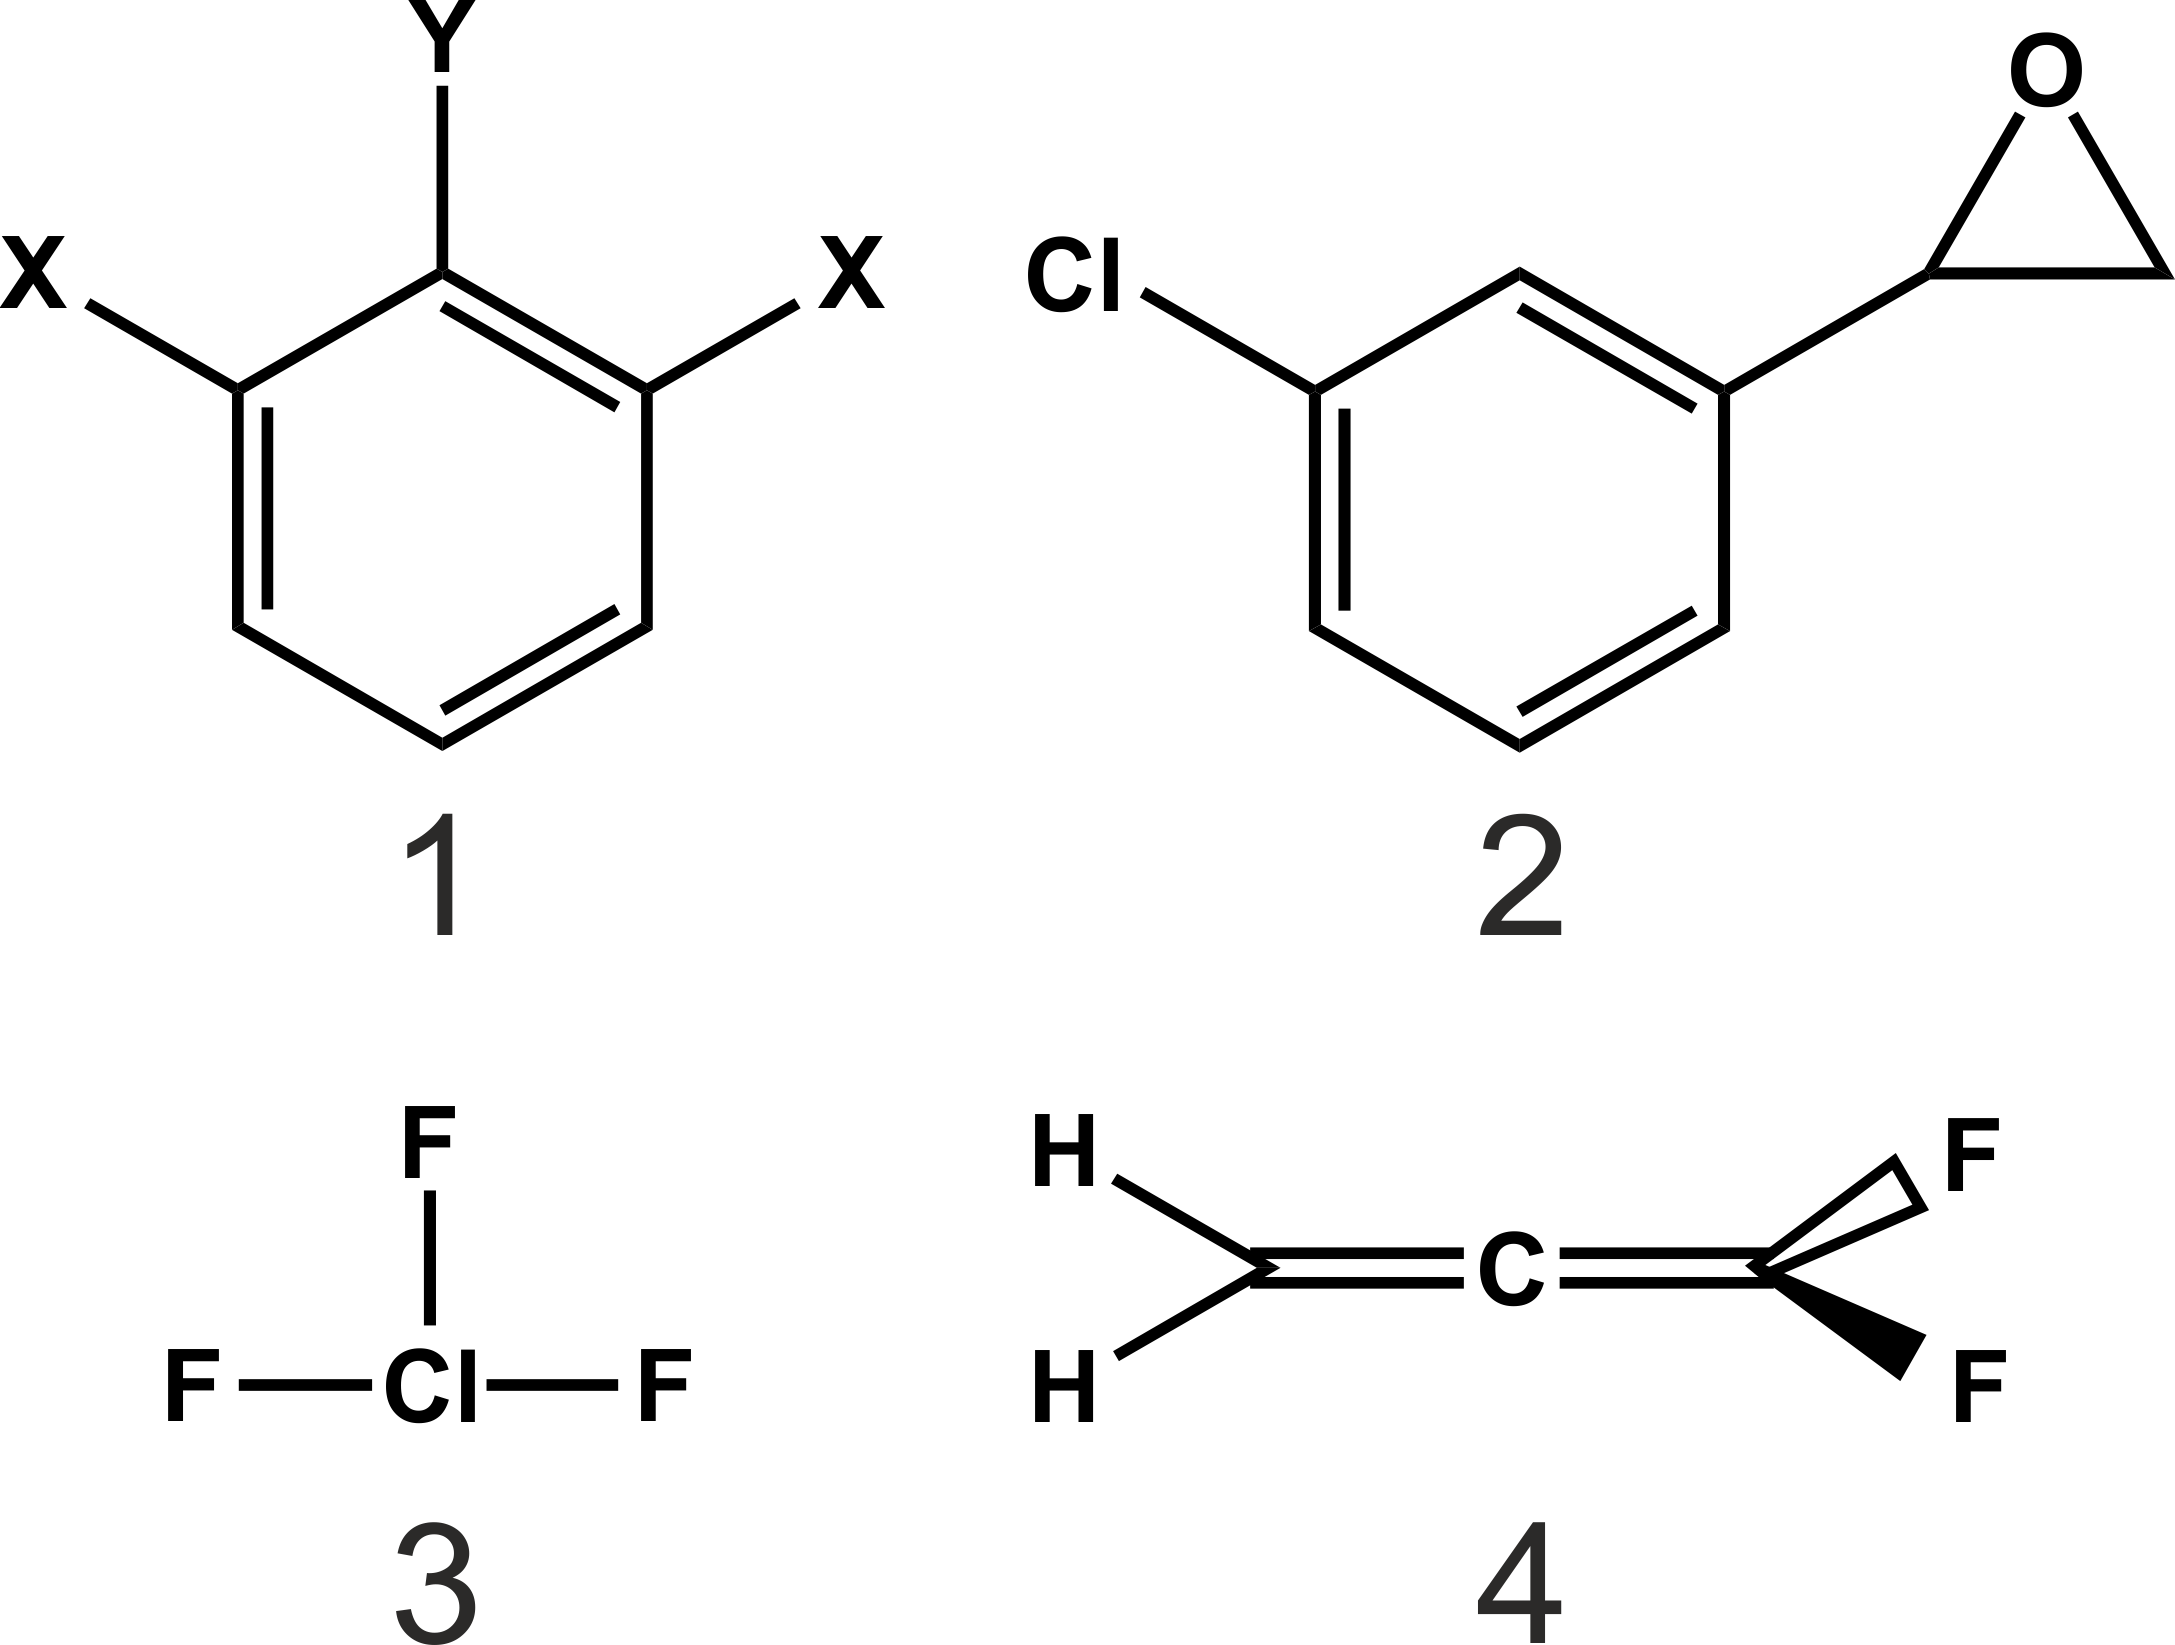
\includegraphics[width=30mm]{images/Fig_2_9_6.png}
    \vspace{-4mm}
\end{wrapfigure}
5К. Нарисуйте спектры ядерного магнитного резонанса (1) A$_2$X$_2$ системы, (2) AMX системы. Какие качественные изменения можно ожидать в спектре AMX системы при ее переходе в ABX систему? Из~приведенных на рисунке справа молекул 1–4 выберете те, которые могут соответствовать случаям (1)~и (2). Ответ аргументируйте и укажите соответствующие ядра в выбранных молекулах. Заместители X, Y не содержат магнитных ядер.
\par
6С. Для AB системы в ЯМР спектроскопии в отсутствии JJ взаимодействия расстояние между линиями равно $\delta$. При учете спин-спинового взаимодействия крайние линии стали в $n$ раз менее интенсивны центральных. Во сколько раз увеличилась протяженность спектра от крайней линии до крайней по сравнению со случаем отсутствия JJ взаимодействия.
\par
7Т. Изобразите протонный и дейтонный спектры ЯМР $\text{HD}$. Определите константу спин-спинового взаимодействия в $\text{H}_2$, считая, что она пропорциональна произведению констант СТВ рассматриваемых ядер, а линии в протонном спектре ЯМР $\text{HD}$ разнесены на 43,5 Гц.
\par
8Т. Спектр $^1\text{H}$ ЯМР некой молекулы, зарегистрированный в спектрометре с~частотой 500 МГц, состоит из двух линий с химическими сдвигами 0 и 10 м. д. Чему равна протяженность спектра $^1\text{H}$ в герцах? Для чего может быть полезным увеличить частоту ЯМР спектрометра? Чему равна протяженность спектра $^{13}\text{C}$~ЯМР в герцах, если в нем зарегистрированы линии с таким же химическим сдвигом, а ядерные $g$-факторы $^1\text{H}$ и $^{13}\text{C}$ равны 5,586 и 1,405, соответственно.
\par
9С. В спектрах $^1\text{H}$ и $^{13}\text{C}$ ЯМР молекулы с брутто-формулой $\text{C}_{4}\text{H}_{8}\text{O}_{2}$ присутствует одна линия. Определите структурную формулу данного соединения.
\par
\begin{wrapfigure}{r}{40mm} %this figure will be at the right
    \centering
    \vspace{-3mm}
    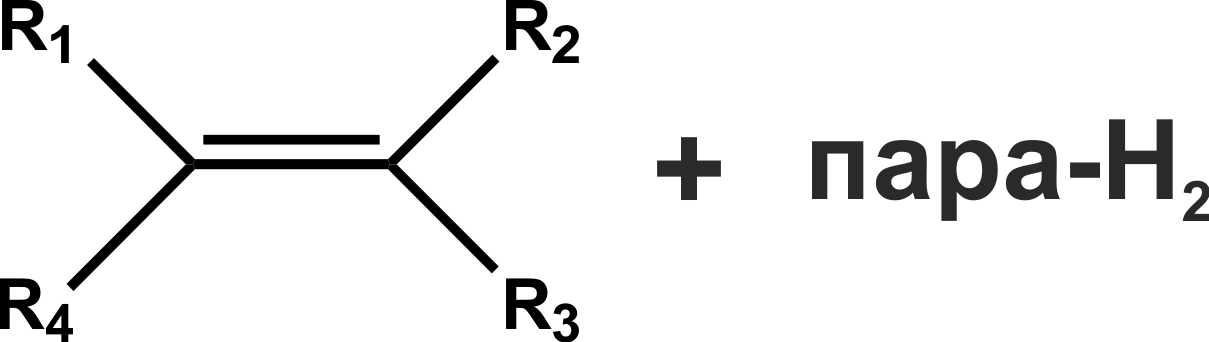
\includegraphics[width=35mm]{images/Fig_2_9_10.png}
    \vspace{-4mm}
\end{wrapfigure}
10К. Нарисуйте $^1\text{H}$ ЯМР спектр реакционной смеси непосредственно после завершения присоединения пара-водорода согласно реакции, приведенной на рисунке. Как будет выглядеть спектр, если подождать значительное время? Считайте, что заместители $\text{R}_i$, $i$ = 1–4 не содержат магнитных ядер и создают значительную разницу в химических сдвигах.
\par
11К. Определите строение соединения с брутто-формулой $\text{C}_{12}\text{H}_{18}\text{O}_{4}$, для которого были зарегистрированы следующие спектры ЯМР: $^1\text{H}$ 1,51 м. д. (с); $^{13}\text{C}$ 150,9; 85,1; 74,0; 27,9 м. д. Укажите также каким именно углеродам соответствуют приведенные значения химического сдвига. Спектр $^{13}\text{C}$ ЯМР получен в условиях подавления спин-спиновых взаимодействий с протонами.
\par
12. Спектр $^1\text{H}$ ЯМР соединения $\text{C}_{18}\text{H}_{18}$ состоит из двух синглетов с химическим сдвигом 8,9 и $-$1,9 м. д. Определите структуру данного соединения.
\par

\chapter[Список теоретических вопросов]{Список теоретических вопросов}
\thispagestyle{empty}

\setmainfont{Noto Serif}
\setsansfont{Noto Sans}
\setmonofont{Noto Sans Mono}
\setstretch{1.35}

\newpage
\section[Описание электронного строения  атомов и молекул]{\texorpdfstring{Описание электронного строения атомов и молекул}{Описание электронного строения  атомов и молекул}}
\textbf{1. Атомы водорода и гелия}\par
1.1П. Атомные орбитали. Визуализация сферических гармоник.\par
1.2. Атом гелия. Расчет энергии основного состояния по теории возмущений.\par
1.3П. Атом гелия. Расчет энергии основного состояния с помошью вариационного метода.\par
1.4. Спин-орбитальное взаимодействие. Природа, гамильтониан, константа.\par
1.5П. Тождественность частиц. Принцип Паули. Детерминант Слейтера.\par
\textbf{2. Многоэлектронные атомы}\par
2.1П. Классификация термов в пределе Рассел-Саундерса. Обозначения термов. Термы электронной конфигурации $p^2$.\par
2.2. Правила Гунда\par
2.3П. Классификация термов в пределе jj-связи. Обозначения термов. Термы электронной конфигурации $p^2$.\par
2.4. Метод Хартри-Фока. Эффективный потенциал.\par
\textbf{3. Переходы между термами}\par
3.1. Правила отбора для электрических дипольных переходов в водородоподобном атоме.\par
3.2П. Правила отбора для электрических дипольных переходов в многоэлектронном атоме.\par
\textbf{4. Многоэлектронный атом во внешних полях}\par
4.1П. Полный магнитный момент атома.\par
4.2П. Многоэлектронный атом в слабом магнитном поле. Эффект Зеемана.\par
4.3П. Многоэлектронный атом в сильном магнитном поле. Эффект Пашена-Бака.\par
4.4. Многоэлектронный атом в электрическом поле. Линейный эффект Штарка.\par
\textbf{5. Электронное строение двухатомных молекул}\par
5.1П. Классификация термов двухатомных молекул.\par
5.2. Сближение атомов с образованием молекулы. Правила Вигнера-Витмера.\par
5.3П. Молекула водорода и ее молекулярные термы.\par
5.4П. Молекула кислорода и ее молекулярные термы.\par
5.5. Правила отбора для электрических дипольных переходов в двухатомных молекулах\par
\textbf{6. Электронное строение многоатомных молекул}\par
6.1П. Приближение Борна-Оппенгеймера.\par
6.2П. Метод Рэлея-Ритца.\par
6.3П. Молекула водорода. Метод Хюккеля.\par
\textbf{7. Применение теории групп для описания электронного строения молекул}\par
7.1. Правила отбора. Оценка интегралов по теории групп.\par
7.2П. Описание $\pi$-сопряженных систем с помощью метода Хюккеля.\par
7.3. Описание электронного строения молекулы воды на языке теории групп.\par
\textbf{8. Специальные хюккелевские системы}\par
8.1П. Альтернантные системы. Теорема парности. Электронное строение аллильного радикала.\par
8.2П. Графическое представление решений для циклических систем. Электронное строение циклобутадиена.\par
8.3. Линейные системы. Электронное строение бутадиена.\par
\textbf{9. Применение теории возмущений для описания электронного строения молекул}\par
9.1П. Введение гетероатома в $\pi$-систему. Электронное строение пиридина.\par
9.2П. Введение индуктивных заместителей в $\pi$-систему. Электронное строение толуола.\par
9.3П. Направление преимущественного замещения в реакциях $S_NAr$ и $S_EAr$.\par
\textbf{10. Разное}\par
10.1. Непересечение состояний с одинаковой симметрией.\par
10.2. Метод Томаса-Ферми.\par
\textbf{11. Примеры дополнительных вопросов}\par
11.1. Может ли существовать нечетный $S$ терм?\par
11.2. Описать электронное строение молекулы N$_2$ используя теорию МО ЛКАО.\par
11.3. Используя теорию групп опишите электронное строение циклопропенильного радикала.\par
11.4. В какие состояния разрешены электрические дипольные переходы из~состояния $^1\Sigma^+$ в группе симметрии $C_{\infty v}$?\par
11.5. С помощью метода МО ЛКАО покажите, что $\text{He}_2$ неустойчивая, а $\text{He}_2^+$ устойчивая молекула.\par
\newpage

\section[Электронное строение координационных соединений.\\Спектроскопические методы исследования вещества]{\texorpdfstring{Электронное строение координационных соединений.\\Спектроскопические методы исследования вещества}{Электронное строение координационных соединений. Спектроскопические методы исследования вещества}}
\textbf{1. Правила Вудворда-Хоффмана}\par
1.1. Использование представлений симметрии при рассмотрении реакционной способности. Типы реакций. Влияние на стереохимию продукта.\par
1.2П. Описание электроциклических реакций. Кон- и дисротаторные пути протекания реакций.\par
1.3. Описание реакций циклоприсоединения на примере $[2+2]$ циклоприсоединения. Супра-/супра- и супра-/антара- пути протекания реакций.\par
\textbf{2. Строение и спектроскопия координационных соединений}\par
2.1П. Теория кристаллического поля. Гамильтониан, предельные случаи, основные приближения. Разложение Лапласа.\par
2.2. Симметрия сферических гармоник.\par
2.3. Описание электронной конфигурации $d_1$ в среднем поле октаэдрической симметрии. В частности, будет требоваться получить потенциал кристаллического поля или рассчитать расщепление по заданному потенциалу.\par
2.4. Теория поля лигандов. Учет $\sigma$ и $\pi$ орбиталей лигандов.\par
2.5П. Оптические переходы в координационных соединениях. Природа $dd$-пере-ходов.\par
2.6. Диаграммы Танабе-Сугано. Спектрохимический ряд лигандов.\par
\textbf{3. Электронная спектроскопия}\par
3.1П. Процессы, протекающие с молекулой после возбуждения.\par
3.2. Природа интеркомбинационной конверсии.\par
3.3. Принцип Франка-Кондона.\par
3.4П. Анизотропия люминесценции на примере поляризованного по оси $z$ возбуждающего излучения и равномерно распределенного замороженного образца.\par
3.5П. Уравнение Штерна-Фольмера. Время жизни возбужденного состояния.\par
3.6П. Тушение люминесценции. Обмен электронами. Триплет-триплетная аннигиляция.\par
3.7П. Тушение люминесценции. Обмен энергией.\par
3.8. Принцип работы лазера. Трехуровневые и четырехуровневые схемы создания инверсной населенности.\par
\textbf{4. ИК и КР спектроскопии}\par
4.1П. Колебания $N$-атомной молекулы. Гамильтониан, нормальные координаты, гармоническое приближение.\par
4.2. Симметрия колебаний. Характеры всех смещений ядер на примере молекулы воды. Аксиальные и полярные векторы. Классификация колебаний. Вывод строчки характеров не требуется.\par
4.3П. Правила отбора. Фундаментальные частоты, составные частоты, обертона. Примеры характеристических колебаний и их частоты.\par
4.4. Интерферометр Майкельсона. Устройство ИК спектрометра.\par
4.5П. Комбинационное рассеяние света. Рамановская спектроскопия. Правила отбора.\par
4.6. Сравнение разрешенных симметрий колебаний в рамановской и ИК спектроскопии на примере конкретной молекулы.\par
\textbf{5. Эффект Яна-Теллера}\par
5.1. Адиабатическое приближение.\par
5.2. Теорема Яна-Теллера.\par
5.3. Псевдоэффект Яна-Теллера. Динамический и статический эффекты.\par
5.4П. Тетрагональное искажение октаэдрического комплекса с конфигурацией металла $d^9$. Симметрия колебания, приводящего к искажению комплекса.\par
\textbf{6. Вращательная спектроскопия и ее производные}\par
6.1. Классификация молекул по компонентам момента инерции.\par
6.2П. Правила отбора вращательных переходов.\par
6.3. Вращательно-колебательная спектроскопия. P, Q, R-ветви.\par
6.4П. Рамановская вращательная спектроскопия. Ядерная спиновая статистика на примере молекулы водорода. Практические применения пара-водорода.\par
6.5. Оператор перестановки ядер. Классификация вращательных уровней.\par
\textbf{7. ЭПР спектроскопия}\par
7.1П. Основные понятия магнитного резонанса. Резонансные условия в ЭПР и~ЯМР. Численные оценки.\par
7.2П. ЭПР в жидкости. Характерные взаимодействия. Природа контактного сверхтонкого взаимодействия. Правила отбора.\par
7.3П. Спектры ЭПР радикалов с одним ядром: $S = I = 1/2$; $S = 1/2$, $I = 1$. Гамильтониан, структура энергетических уровней.\par
7.4П. Природа контактного СТВ в органических радикалах. Косвенное взаимодействие. Соотношение Мак-Коннела.\par
7.5П. Природа контактного СТВ в органических радикалах. Сверхсопряжение.\par
\textbf{8. Химический обмен в магнитом резонансе}\par
8.1. Ларморовская прецессия спина в магнитном поле.\par
8.2. Проявление обмена в спектрах ЭПР. Медленный и быстрый обмен, описание трансформации спектра на конкретном примере.\par
8.3. Обмен по многим положениям. Реакции вырожденного электронного обмена.\par
8.4. Поправка к энергии ЭПР перехода во втором порядке теории возмущений. Спектр $^{\boldsymbol{\cdot}}\text{CF}_3$ радикала с ее учетом.\par
\textbf{9. ЯМР спектроскопия}\par
9.1П. Гамильтониан и химический сдвиг. Природа химического сдвига. Демонстрация эффекта электроотрицательности соседних групп.\par
9.2П. Спектр ЯМР АХ системы. Как будет выглядеть спектр ЯМР $\text{A}_{\text{n}}\text{X}_{\text{m}}$ системы?\par
9.3. Химические сдвиги $^1$Н ЯМР спектроскопии. Основные факторы. Магнитная анизотропия соседних групп на примере ароматических соединений.\par
9.4. Спектр ЯМР АB системы.\par
9.5П. Особенности спектроскопии $^{13}$С ЯМР. Пример спектра $^{13}$С ЯМР соединения на выбор.\par
\textbf{10. Примеры дополнительных вопросов}\par
10.1. Гомоядерные двухатомные молекулы с нулевым ядерным спином могут иметь либо четные, либо нечетные вращательные уровни. Можно ли установить четность, исходя из вращательных спектров комбинационного рассеяния?\par
10.2. Спектр $^{1}$Н ЯМР некой молекулы, зарегистрированный в спектрометре с~частотой 400 МГц, состоит из двух линий с химическим сдвигом 0 м. д. и~10~м.~д. Чему равна протяженность спектра в герцах? На что влияет увеличение частоты ЯМР спектрометра?\par
10.3. Спектры поглощения комплексов $[\text{PtBr}_4]^{2-}$ и $[\text{PtCl}_4]^{2-}$ похожи. Однако полоса переноса заряда от лиганда к центральному иону в $[\text{PtBr}_4]^{2-}$ сдвинута в красную область, и соответствующая энергия перехода равна 36000 см$^{-1}$, в то время как для $[\text{PtCl}_4]^{2-}$ эта величина равна 44000 см$^{-1}$. Какова природа наблюдаемого сдвига?\par
10.4. Расщепление на $\beta$-протонах в спектре ЭПР этильного радикала составляет 26,87 Гс. Чему равна спиновая плотность на $1s$ орбитали $\beta$-атома водорода.\par
10.5. Определить число четных и нечетных колебаний для линейной $N$-атомной молекулы с центром инверсии.\par
10.6. Может ли в реакции $[2+2]$ циклоприсоединения двух этиленов, протекающей фотохимически в супра-/супра- топологии, получиться электронно-возбужденная молекула циклобутана?\par
10.7. Почему во вращательно-колебательном спектре молекулы NO есть Q-ветвь, а в аналогичном спектре HCl ее нет. Определите основные термы данных молекул.\par




% Appendices section.
%\appendix

% Include the foreword page from the FrontMatter subfolder.
\chapter{Справочные данные}
%\addcontentsline{toc}{chapter}{Справочные данные}
\thispagestyle{empty}
\setmainfont{Noto Serif}
\setsansfont{Noto Sans}
\setmonofont{Noto Sans Mono}
\setstretch{1.15}

%\phantomsection
\section{Вид некоторых сферических гармоник}
%\addcontentsline{toc}{section}{Вид некоторых сферических гармоник}
%\markboth{Вид некоторых сферических гармоник}{Вид некоторых сферических гармоник}
\rule{\textwidth}{0.4pt}
\[ \textit{Y}_{00}=\sqrt{\frac{1}{4\pi}};\]
\rule{\textwidth}{0.4pt}
\[\textit{Y}_{10}=\frac{1}{2}\sqrt{\frac{3}{\pi}}\cos {\theta}; \quad \textit{Y}_{11}=-\frac{1}{2}\sqrt{\frac{3}{2\pi}}\sin{\theta} \, e^{\,i\phi};\quad \textit{Y}_{1-1}=\frac{1}{2}\sqrt{\frac{3}{2\pi}}\sin{\theta} \, e^{-i\phi}; \]
\rule{\textwidth}{0.4pt}
\[ \textit{Y}_{20}=\frac{1}{4}\sqrt{\frac{5}{\pi}}\left( 3 \cos^2{\theta}-1 \right);\] 
\[\textit{Y}_{21}=-\frac{1}{2}\sqrt{\frac{15}{2\pi}}\cos{\theta} \sin{\theta}\, e^{\,i\phi};\quad \textit{Y}_{2-1}=\frac{1}{2}\sqrt{\frac{15}{2\pi}}\cos{\theta} \sin{\theta}\, e^{-i\phi};
\]\hspace{\parindent}
\[ \textit{Y}_{22}=\frac{1}{4}\sqrt{\frac{15}{2\pi}} \sin^2 {\theta} \, e^{\,2i\phi}; \quad
\textit{Y}_{2-2}=\frac{1}{4}\sqrt{\frac{15}{2\pi}} \sin^2 {\theta} \, e^{-2i\phi};
\]
\rule{\textwidth}{0.4pt}
\[ \textit{Y}_{30}=\frac{1}{4}\sqrt{\frac{7}{\pi}}\left(5 \cos^3{\theta}-3\cos{\theta} \right);\ \]
\[\textit{Y}_{31}=-\frac{1}{8}\sqrt{\frac{21}{\pi}}\left(5\cos^2{\theta}-1 \right)\sin{\theta}\, e^{\,i\phi};\quad \textit{Y}_{3-1}=\frac{1}{8}\sqrt{\frac{21}{\pi}}\left( 5\cos^2{\theta}-1 \right)\sin{\theta}\, e^{-i\phi};
\]\hspace{\parindent}
\[\textit{Y}_{32}=\frac{1}{4}\sqrt{\frac{105}{2\pi}}\cos{\theta} \sin^2{\theta}\, e^{\,2i\phi};\quad \textit{Y}_{3-2}=\frac{1}{4}\sqrt{\frac{105}{2\pi}}\cos{\theta} \sin^2{\theta}\, e^{-2i\phi};
\]\hspace{\parindent}
\[ \textit{Y}_{33}=-\frac{1}{8}\sqrt{\frac{35}{\pi}} \sin^3 {\theta} \, e^{\,3i\phi}; \quad
\textit{Y}_{3-3}=\frac{1}{8}\sqrt{\frac{35}{\pi}} \sin^3 {\theta} \, e^{-3i\phi};
\]
\rule{\textwidth}{0.4pt}
\[ \textit{Y}_{40}=\frac{3}{16}\sqrt{\frac{1}{\pi}}\left(35 \cos^4{\theta}-30\cos^2{\theta}+3 \right);\ \]
\[\textit{Y}_{41}=-\frac{3}{8}\sqrt{\frac{5}{\pi}} \left(7\cos^3{\theta}-3\cos{\theta}\right)\sin{\theta}\, e^{\,i\phi};\; \textit{Y}_{4-1}=\frac{3}{8}\sqrt{\frac{5}{\pi}}\left(7\cos^3{\theta}-3\cos{\theta}\right)\sin{\theta}\, e^{-i\phi};
\]\hspace{\parindent}
\[\textit{Y}_{42}=\frac{3}{8}\sqrt{\frac{5}{2\pi}}\left(7\cos^2{\theta}-1 \right) \sin^2{\theta}\, e^{\,2i\phi};\quad \textit{Y}_{4-2}=\frac{3}{8}\sqrt{\frac{5}{2\pi}}\left(7\cos^2{\theta}-1 \right) \sin^2{\theta}\, e^{-2i\phi};
\]\hspace{\parindent}
\[\textit{Y}_{43}=-\frac{3}{8}\sqrt{\frac{35}{\pi}}\cos{\theta} \sin^3{\theta}\, e^{\,3i\phi};\quad \textit{Y}_{4-3}=\frac{3}{8}\sqrt{\frac{35}{\pi}}\cos{\theta} \sin^3{\theta}\, e^{-3i\phi};
\]\hspace{\parindent}
\[ \textit{Y}_{44}=\frac{3}{16}\sqrt{\frac{35}{2\pi}} \sin^4 {\theta} \, e^{\,4i\phi}; \quad
\textit{Y}_{4-4}=\frac{3}{16}\sqrt{\frac{35}{2\pi}} \sin^4 {\theta} \, e^{-4i\phi};
\]
\rule{\textwidth}{0.4pt}

%\phantomsection
\section{Действительный вид некоторых сферических гармоник}
%\addcontentsline{toc}{section}{Действительный вид некоторых сферических гармоник}
%\markboth{Действительный вид некоторых сферических гармоник}{Действительный вид некоторых сферических гармоник}
\rule{\textwidth}{0.4pt}
\[ s=\textit{Y}_{00}=\sqrt{\frac{1}{4\pi}};\]
\rule{\textwidth}{0.4pt}
\[ p_z=\textit{Y}_{10}=\sqrt{\frac{3}{4\pi}}\,\frac{z}{r}; \] 
\[p_x=\sqrt{\frac{1}{2}}\left(\textit{Y}_{1-1}-\textit{Y}_{11}\right)=\sqrt{\frac{3}{4\pi}}\,\frac{x}{r}; \quad p_y=i\sqrt{\frac{1}{2}}(\textit{Y}_{1-1}+\textit{Y}_{11})=\sqrt{\frac{3}{4\pi}}\,\frac{y}{r}; \]
\rule{\textwidth}{0.4pt}
\[ d_{z^2}=\textit{Y}_{20}=\frac{1}{4}\sqrt{\frac{5}{\pi}}\,\frac{3z^2-r^2}{r^2}; \] 
\[d_{xz}=\sqrt{\frac{1}{2}}(\textit{Y}_{2-1}-\textit{Y}_{21})=\frac{1}{2}\sqrt{\frac{15}{\pi}}\,\frac{xz}{r^2}; \quad d_{yz}=i\sqrt{\frac{1}{2}}(\textit{Y}_{2-1}+\textit{Y}_{21})=\frac{1}{2}\sqrt{\frac{15}{\pi}}\,\frac{yz}{r^2}; \]\hspace{\parindent}
\[d_{x^2-y^2}=\sqrt{\frac{1}{2}}(\textit{Y}_{2-2}+\textit{Y}_{22})=\frac{1}{4}\sqrt{\frac{15}{\pi}}\,\frac{x^2-y^2}{r^2}; \quad d_{xy}=i\sqrt{\frac{1}{2}}(\textit{Y}_{2-2}-\textit{Y}_{22})=\frac{1}{2}\sqrt{\frac{15}{\pi}}\,\frac{xy}{r^2}; \]
\rule{\textwidth}{0.4pt}
\[ f_{z^3}=\textit{Y}_{30}=\frac{1}{4}\sqrt{\frac{7}{\pi}}\,\frac{z(5z^2-3r^2)}{r^3}; \] 
\[f_{xz^2}=\sqrt{\frac{1}{2}}(\textit{Y}_{3-1}-\textit{Y}_{31})=\frac{1}{4}\sqrt{\frac{21}{2\pi}}\,\frac{x(5z^2-r^2)}{r^3}; \]\hspace{\parindent}
\[ f_{yz^2}=i\sqrt{\frac{1}{2}}(\textit{Y}_{3-1}+\textit{Y}_{31})=\frac{1}{4}\sqrt{\frac{21}{2\pi}}\,\frac{y(5z^2-r^2)}{r^3}; \]\hspace{\parindent}
\[f_{xyz}=i\sqrt{\frac{1}{2}}(\textit{Y}_{3-2}-\textit{Y}_{32})=\frac{1}{2}\sqrt{\frac{105}{\pi}}\,\frac{xyz}{r^3}; \] \hspace{\parindent}
\[ f_{z(x^2-y^2)}=\sqrt{\frac{1}{2}}(\textit{Y}_{3-2}+\textit{Y}_{32})=\frac{1}{4}\sqrt{\frac{105}{\pi}}\,\frac{z(x^2-y^2)}{r^3}; \] \hspace{\parindent}
\[f_{y(3x^2-y^2)}=i\sqrt{\frac{1}{2}}(\textit{Y}_{3-3}+\textit{Y}_{33})=\frac{1}{4}\sqrt{\frac{35}{2\pi}}\,\frac{y(3x^2-y^2)}{r^3}; \] \hspace{\parindent}
\[f_{x(x^2-3y^2)}=\sqrt{\frac{1}{2}}(\textit{Y}_{3-3}-\textit{Y}_{33})=\frac{1}{4}\sqrt{\frac{35}{2\pi}}\,\frac{x(x^2-3y^2)}{r^3}; \]
\rule{\textwidth}{0.4pt}

\setstretch{1.55}

%\phantomsection
\section{Некоторые таблицы характеров}
%\addcontentsline{toc}{section}{Некоторые таблицы характеров}
%\markboth{Некоторые таблицы характеров}{Некоторые таблицы характеров}
\begin{center}
\begin{tabular}{ |c|c|c|c|c|c| }
 \hline
 $C_{2v}$ & $E$ & $C_2^z$ & $\sigma_v^{xz}$ & $\sigma_v^{yz}$ & $h=4$ \\ 
 \hline
 $A_1$ & 1 & 1 & 1 & 1 & $z,\,x^2,\,y^2,\,z^2$ \\  
 \hline
 $A_2$ & 1 & 1 & $-1$ & $-1$ & $R_z,\,xy$ \\
 \hline
 $B_1$ & 1 & $-1$ & $1$ & $-1$ & $x,\,R_y,\,xz$ \\
 \hline
 $B_2$ & 1 & $-1$ & $-1$ & $1$ & $y,\,R_x,\,yz$ \\
 \hline
\end{tabular}
\end{center}

\begin{center}
\begin{tabular}{ |c|c|c|c|c| }
 \hline
 $C_{3v}$ & $E$ & $2C_3^z$ & $3\sigma_v$ & $h=6$ \\ 
 \hline
 $A_1$ & 1 & 1 & 1 & $z,\,x^2+y^2,\,z^2$ \\  
 \hline
 $A_2$ & 1 & 1 & $-1$ & $R_z$ \\
 \hline
 $E$ & 2 & $-1$ & $0$ & \begin{tabular}{@{}c@{}} $(x,y),\, (R_x,\,R_y)$ \\ $(x^2-y^2,\,xy),\,(xz,\,yz)$\end{tabular} \\
 \hline
\end{tabular}
\end{center}

\begin{center}
\begin{tabular}{ |c|c|c|c|c|c|c| }
 \hline
 $C_{4v}$ & $E$ & $2C_4^z$ & $C_2^z$ & $2\sigma_v$ & $2\sigma_d$ & $h=8$ \\ 
 \hline
 $A_1$ & 1 & 1 & 1 & 1 & 1 & $z,\,x^2+y^2,\,z^2$ \\  
 \hline
 $A_2$ & 1 & 1 & $1$ & $-1$ & $-1$ & $R_z$ \\
 \hline
 $B_1$ & 1 & $-1$ & 1 & 1 & $-1$ & $x^2-y^2$ \\  
 \hline
 $B_2$ & 1 & $-1$ & $1$ & $-1$ & $1$ & $xy$ \\
 \hline
 $E$ & 2 & $0$ & $-2$ & $0$ & $0$ & \begin{tabular}{@{}c@{}} $(x,y),\, (R_x,\,R_y)$ \\ $(xz,\,yz)$\end{tabular} \\
 \hline
\end{tabular}
\end{center}

\begin{center}
\begin{tabular}{ |c|c|c|c|c| }
 \hline
 $C_{\infty v}$ & $E$ & $2C_{\infty}$ & $\infty\sigma_v$ & $h=\infty$ \\ 
 \hline
 $\Sigma^+$ & 1 & 1 & 1 & $z,\,x^2+y^2,\,z^2$ \\  
 \hline
 $\Sigma^-$ & 1 & 1 & $-1$ & $R_z$ \\
 \hline
 $\Pi$ & 2 & $2\cos{\phi}$ & $0$ & \begin{tabular}{@{}c@{}} $(x,y),\, (R_x,\,R_y)$ \\ $(xz,\,yz)$\end{tabular} \\
 \hline
 $\Delta$ & 2 & $2\cos{2\phi}$ & $0$ & $(x^2-y^2,\,xy)$ \\
 \hline
 $\Phi$ & 2 & $2\cos{3\phi}$ & $0$ & $-$ \\
 \hline
 $\ldots$ & $\ldots$ & $\ldots$ & $\ldots$ & $-$ \\
 \hline
 $E_n$ & 2 & $2\cos{n\phi}$ & $0$ & $-$ \\
 \hline
\end{tabular}
\end{center}

\begin{center}
\begin{tabular}{ |c|c|c|c|c|c|c| }
 \hline
 $D_{2d}$ & $E$ & $2S_4$ & $C_2^z$ & $2C'_2$ & $2\sigma_d$ & $h=8$ \\ 
 \hline
 $A_1$ & 1 & 1 & 1 & 1 & 1 & $x^2+y^2,\,z^2$ \\  
 \hline
 $A_2$ & 1 & 1 & $1$ & $-1$ & $-1$ & $R_z$ \\
 \hline
 $B_1$ & 1 & $-1$ & 1 & 1 & $-1$ & $x^2-y^2$ \\  
 \hline
 $B_2$ & 1 & $-1$ & $1$ & $-1$ & $1$ & $z,\,xy$ \\
 \hline
 $E$ & 2 & $0$ & $-2$ & $0$ & $0$ & \begin{tabular}{@{}c@{}} $(x,y),\, (R_x,\,R_y)$ \\ $(xz,\,yz)$\end{tabular} \\
 \hline
\end{tabular}
\end{center}

\begin{center}
\begin{tabular}{ |c|c|c|c|c|c|c|c|c|c| }
 \hline
 $D_{2h}$ & $E$ & $C_2^z$ & $C_2^y$ & $C_2^x$ & $I$ & $\sigma_{xy}$ & $\sigma_{xz}$ & $\sigma_{yz}$ & $h=8$ \\ 
 \hline
 $A_g$ & 1 & 1 & 1 & 1 & 1 & 1 & 1 & 1 & $x^2,\,y^2,\,z^2$ \\  
 \hline
 $B_{1g}$ & 1 & 1 & $-1$ & $-1$ & $1$ & $1$ & $-1$ & $-1$ & $R_z$,\,$xy$ \\
 \hline
 $B_{2g}$ & 1 & $-1$ & $1$ & $-1$ & $1$ & $-1$ & $1$ & $-1$ & $R_y$,\,$xz$ \\
 \hline
 $B_{3g}$ & 1 & $-1$ & $-1$ & $1$ & $1$ & $-1$ & $-1$ & $1$ & $R_x$,\,$yz$ \\
 \hline
 $A_u$ & 1 & 1 & 1 & 1 & $-1$ & $-1$ & $-1$ & $-1$ & $-$ \\  
 \hline
 $B_{1u}$ & 1 & 1 & $-1$ & $-1$ & $-1$ & $-1$ & $1$ & $1$ & $z$ \\
 \hline
 $B_{2u}$ & 1 & $-1$ & $1$ & $-1$ & $-1$ & $1$ & $-1$ & $1$ & $y$ \\
 \hline
 $B_{3u}$ & 1 & $-1$ & $-1$ & $1$ & $-1$ & $1$ & $1$ & $-1$ & $x$ \\
 \hline
\end{tabular}
\end{center}

\begin{center}
\begin{tabular}{ |c|c|c|c|c|c|c|c| }
 \hline
 $D_{3h}$ & $E$ & $2C_3^z$ & $3C'_2$ & $\sigma_h^{xy}$ & $2S_{3}$ & $3\sigma_{v}$ & $h=12$ \\ 
 \hline
 $A'_1$ & 1 & 1 & 1 & 1 & 1 & 1 & $x^2+y^2,\,z^2$ \\  
 \hline
 $A'_{2}$ & 1 & 1 & $-1$ & $1$ & $1$ & $-1$ & $R_z$ \\
 \hline
 $E'$ & 2 & $-1$ & $0$ & $2$ & $-1$ & $0$ & $(x,\,y),\,(x^2-y^2,\,xy)$ \\
 \hline
 $A''_{1}$ & 1 & $1$ & $1$ & $-1$ & $-1$ & $-1$ & $-$ \\
 \hline
 $A''_2$ & 1 & 1 & $-1$ & $-1$ & $-1$ & $1$ &  $z$ \\  
 \hline
 $E''$ & 2 & $-1$ & $0$ & $-2$ & $1$ & $0$ & $(R_x,\,R_y),\,(xz,\,yz)$ \\
 \hline
\end{tabular}
\end{center}

\begin{center}
\begin{tabular}{ |c|c|c|c|c|c|c| }
 \hline
 $T_{d}$ & $E$ & $8C_3$ & $3C_2$ & $6S_4$ & $6\sigma_d$ & $h=24$ \\ 
 \hline
 $A_1$ & 1 & 1 & 1 & 1 & 1 & $r^2$ \\  
 \hline
 $A_2$ & 1 & 1 & $1$ & $-1$ & $-1$ & $-$ \\
 \hline
 $E$ & 2 & $-1$ & 2 & 0 & $0$ & $(3z^2-r^2,\,x^2-y^2)$ \\  
 \hline
 $T_1$ & 3 & $0$ & $-1$ & $1$ & $-1$ & $\vec{R}$ \\
 \hline
 $T_2$ & 3 & $0$ & $-1$ & $-1$ & $1$ & $\vec{r},\,(xy,\,xz,\,yz)$ \\
 \hline
\end{tabular}
\end{center}

\begin{center}
\begin{tabular}{ |c|c|c|c|c|c|c|c|c|c|c|c| }
 \hline
 $D_{4h}$ & $E$ & $2C_4^z$ & $C_2^z$ & $2C_2'$ & $2C_2''$ & $I$ & $2S_{4}$ & $\sigma_{h}$ & 2$\sigma_{v}$ & 2$\sigma_{d}$ & $h=16$ \\ 
 \hline
 $A_{1g}$ & 1 & 1 & 1 & 1 & 1 & 1 & 1 & 1 & 1 & 1 & $x^2+y^2,\,z^2$ \\  
 \hline
 $A_{2g}$ & 1 & 1 & $1$ & $-1$ & $-1$ & 1 & 1 & $1$ & $-1$ & $-1$ & $R_z$ \\
 \hline
 $B_{1g}$ & 1 & $-1$ & $1$ & $1$ & $-1$ & 1 & $-1$ & $1$ & $1$ & $-1$ & $x^2-y^2$ \\  
 \hline
 $B_{2g}$  & 1 & $-1$ & $1$ & $-1$ & $1$ & 1 & $-1$ & $1$ & $-1$ & $1$ & $xy$ \\
 \hline 
 $E_g$ & 2 & $0$ & $-2$ & $0$ & $0$ & 2 & $0$ & $-2$ & $0$ & $0$ & \begin{tabular}{@{}c@{}} $(R_x,\,R_y)$ \\ $(xz,\,yz)$\end{tabular} \\
 \hline
 $A_{1u}$ & 1 & $1$ & $1$ & $1$ & $1$ & $-1$ & $-1$ & $-1$ & $-1$ & $-1$ & $-$ \\
 \hline
 $A_{2u}$ & 1 & 1 & $1$ & $-1$ & $-1$ & $-1$ & $-1$ & $-1$ & $1$ & $1$ &  $z$ \\  
 \hline
 $B_{1u}$ & 1 & $-1$ & $1$ & $1$ & $-1$ & $-1$ & $1$ & $-1$ & $-1$ & $1$ & $-$ \\
 \hline
 $B_{2u}$ & 1 & $-1$ & $1$ & $-1$ & $1$ & $-1$ & $1$ & $-1$ & $1$ & $-1$ & $-$ \\  
 \hline
 $E_u$ & 2 & $0$ & $-2$ & $0$ & $0$ & $-2$ & $0$ & $2$ & $0$ & $0$ & $(x,\,y)$ \\
 \hline 
\end{tabular}
\end{center}
При наличии в группе симметрии одновременно осей симметрии $C_2'$ и $C_2''$ считать, что оси $C_2'$ направлены на атомы, а оси $C_2''$ направлены между атомами. Отражения в плоскости $\sigma_v$, $\sigma_d$ в этом случае содержат оси симметрии $C_2'$, $C_2''$, соответственно.

\begin{center}
\begin{tabular}{ |c|c|c|c|c|c|c|c| }
 \hline
 $D_{\infty h}$ & $E$ & $2C_{\infty}$ & $\infty\sigma_v$ & $I$ & $2S_\infty$ & $\infty C_2'$ & $h=\infty$ \\ 
 \hline
 $\Sigma^+_g$ & 1 & 1 & 1 & 1 & 1 & 1 & $x^2+y^2,\,z^2$ \\  
 \hline
 $\Sigma^-_g$ & 1 & 1 & $-1$ & 1 & 1 & $-1$ & $R_z$ \\
 \hline
 $\Pi_g$ & 2 & $2\cos{\phi}$ & $0$ & 2 & $-2\cos{\phi}$ & $0$ & $(R_x,\,R_y),\,(xz,\,yz)$ \\
 \hline
 $\Delta_g$ & 2 & $2\cos{2\phi}$ & $0$ & 2 & $2\cos{2\phi}$ & $0$ & $(x^2-y^2,\,xy)$ \\
 \hline
 $\Phi_g$ & 2 & $2\cos{3\phi}$ & $0$ & 2 & $-2\cos{3\phi}$ & $0$ & $-$ \\
 \hline
 $\ldots$ & $\ldots$ & $\ldots$ & $\ldots$ & $\ldots$ & $\ldots$ & $\ldots$ & $-$ \\
 \hline
 $E_{ng}$ & 2 & $2\cos{n\phi}$ & $0$ & 2 & $(-1)^n\,2\cos{n\phi}$ & $0$ & $-$ \\
 \hline
 $\Sigma^+_u$ & 1 & 1 & 1 & $-1$ & $-1$ & $-1$ & $z$ \\  
 \hline
 $\Sigma^-_u$ & 1 & 1 & $-1$ & $-1$ & $-1$ & $1$ & $-$ \\
 \hline
 $\Pi_u$ & 2 & $2\cos{\phi}$ & $0$ & $-2$ & $2\cos{\phi}$ & $0$ & $(x,\,y)$ \\
 \hline
 $\Delta_u$ & 2 & $2\cos{2\phi}$ & $0$ & $-2$ & $-2\cos{2\phi}$ & $0$ & $-$ \\
 \hline
 $\Phi_u$ & 2 & $2\cos{3\phi}$ & $0$ & $-2$ & $2\cos{3\phi}$ & $0$ & $-$ \\
 \hline
 $\ldots$ & $\ldots$ & $\ldots$ & $\ldots$ & $\ldots$ & $\ldots$ & $\ldots$ & $-$ \\
 \hline
 $E_{nu}$ & 2 & $2\cos{n\phi}$ & $0$ & $-2$ & $(-1)^{n+1}\,2\cos{n\phi}$ & $0$ & $-$ \\
 \hline
\end{tabular}
\end{center}

\begin{center}
\begin{tabular}{ |c|c|c|c|c|c|c|c|c|c|c|c| }
 \hline
 $O_{h}$ & $E$ & $8C_3$ & $6C_2$ & $6C_4^z$ & $3C_2^z$ & $I$ & $6S_{4}$ & $8S_{6}$ & 3$\sigma_{h}$ & 6$\sigma_{d}$ & $h=48$ \\ 
 \hline
 $A_{1g}$ & 1 & 1 & 1 & 1 & 1 & 1 & 1 & 1 & 1 & 1 & $r^2$ \\  
 \hline
 $A_{2g}$ & 1 & 1 & $-1$ & $-1$ & $1$ & 1 & $-1$ & $1$ & $1$ & $-1$ & $-$ \\
 \hline
 $E_{g}$ & 2 & $-1$ & $0$ & $0$ & $2$ & 2 & $0$ & $-1$ & $2$ & $0$ & \begin{tabular}{@{}c@{}} $(3z^2-r^2,$\\$x^2-y^2)$\end{tabular} \\  
 \hline
 $T_{1g}$  & 3 & $0$ & $-1$ & $1$ & $-1$ & 3 & $1$ & $0$ & $-1$ & $-1$ & $\vec{R}$ \\
 \hline 
 $T_{2g}$ & 3 & $0$ & $1$ & $-1$ & $-1$ & 3 & $-1$ & $0$ & $-1$ & $1$ &  \fontsize{7.82}{7.82}$(xz,yz,xy)$ \\
 \hline
 $A_{1u}$ & 1 & $1$ & $1$ & $1$ & $1$ & $-1$ & $-1$ & $-1$ & $-1$ & $-1$ & $-$ \\
 \hline
 $A_{2u}$ & 1 & 1 & $-1$ & $-1$ & $1$ & $-1$ & $1$ & $-1$ & $-1$ & $1$ &  $-$ \\  
 \hline
 $E_{u}$ & 2 & $-1$ & $0$ & $0$ & $2$ & $-2$ & $0$ & $1$ & $-2$ & $0$ & $-$ \\
 \hline
 $T_{1u}$ & 3 & $0$ & $-1$ & $1$ & $-1$ & $-3$ & $-1$ & $0$ & $1$ & $1$ & $\vec{r}$ \\  
 \hline
 $T_{2u}$ & 3 & $0$ & $1$ & $-1$ & $-1$ & $-3$ & $1$ & $0$ & $1$ & $-1$ & $-$ \\
 \hline 
\end{tabular}
\end{center}

%\newpage


\setstretch{1.35}

%\phantomsection
\section{Эквивалентные операторы для интегралов с \texorpdfstring{$\textit{Y}_{2m}$}{|2 m>}}
%\addcontentsline{toc}{section}{Эквивалентные операторы для интегралов с $\textit{Y}_{2m}$}
%\markboth{Эквивалентные операторы для интегралов с $\textit{Y}_{2m}$}{Эквивалентные операторы для интегралов с $\textit{Y}_{2m}$}
\rule{\textwidth}{0.4pt}
\[ \widehat L_{40} = \frac{1}{168}\sqrt{\frac{1}{\pi}}\left( 35\widehat L_z^4-30\widehat L_z^2 \widehat L^2+25\widehat L_z^2-6\widehat L^2+3 (\widehat L^2)^2 \right); \quad \widehat L_{44} =\frac{1}{168}\sqrt{\frac{35}{2\pi}} \left( \widehat L_+^4 + \widehat L_-^4  \right);\]\hspace{\parindent}
%\rule{\textwidth}{0.4pt}
\[ \widehat L_{41} = -\frac{1}{168}\sqrt{\frac{5}{\pi}} \left( (\widehat L_+ + \widehat L_- )(7\widehat L_z^3 - (3\widehat L^2 + 1)\widehat L_z) + (7\widehat L_z^3 - (3\widehat L^2 + 1)\widehat L_z)(\widehat L_+ + \widehat L_- ) \right); \]\hspace{\parindent}
%\rule{\textwidth}{0.4pt}
\[ \widehat L_{42} =\frac{1}{168}\sqrt{\frac{5}{2\pi}} \left( (\widehat L_+^2 + \widehat L_-^2 )(7\widehat L_z^2 - \widehat L^2 - 5) + (7\widehat L_z^2 - \widehat L^2  - 5)(\widehat L_+^2 + \widehat L_-^2 ) \right); \]\hspace{\parindent}
%\rule{\textwidth}{0.4pt}
\[ \widehat L_{43} =-\frac{1}{24}\sqrt{\frac{5}{7\pi}} \left( (\widehat L_+^3 + \widehat L_-^3 )\widehat L_z + \widehat L_z (\widehat L_+^3 + \widehat L_-^3 ) \right); \]
%\rule{\textwidth}{0.4pt}
%\[ \widehat L_{44} =\frac{1}{168}\sqrt{\frac{35}{2\pi}} \left( \widehat L_+^4 + \widehat L_-^4  \right);\]
\rule{\textwidth}{0.4pt}
\[ \widehat L_{20} = -\frac{1}{42}\sqrt{\frac{5}{\pi}}\left(3\widehat L_z^2-\widehat L^2\right); \quad \widehat L_{22} =-\frac{1}{14}\sqrt{\frac{5}{6\pi}} \left( \widehat L_+^2 + \widehat L_-^2  \right); \]\hspace{\parindent}
%\rule{\textwidth}{0.4pt}
\[ \widehat L_{21} = \frac{1}{14}\sqrt{\frac{5}{6\pi}}\left(\widehat L_z (\widehat L_+ + \widehat L_-)+(\widehat L_+ + \widehat L_-) \widehat L_z\right);\]
\rule{\textwidth}{0.4pt}
%\[ \widehat L_{22} =-\frac{1}{14}\sqrt{\frac{5}{6\pi}} \left( \widehat L_+^2 + \widehat L_-^2  \right); \]
%\rule{\textwidth}{0.4pt}

%\phantomsection
\section{Эквивалентные операторы для интегралов с \texorpdfstring{$\textit{Y}_{1m}$}{|1 m>}}
%\addcontentsline{toc}{section}{Эквивалентные операторы для интегралов с $\textit{Y}_{1m}$}
%\markboth{Эквивалентные операторы для интегралов с $\textit{Y}_{1m}$}{Эквивалентные операторы для интегралов с $\textit{Y}_{1m}$}
\rule{\textwidth}{0.4pt}
\[ \widehat L_{20} = -\frac{1}{2}\sqrt{\frac{1}{5\pi}}\left(3\widehat L_z^2-\widehat L^2\right); \quad \widehat L_{22} =-\frac{1}{2}\sqrt{\frac{3}{10\pi}} \left( \widehat L_+^2 + \widehat L_-^2  \right);\]\hspace{\parindent}
%\rule{\textwidth}{0.4pt}
\[ \widehat L_{21} = \frac{1}{2}\sqrt{\frac{3}{10\pi}}\left(\widehat L_z (\widehat L_+ + \widehat L_-)+(\widehat L_+ + \widehat L_-) \widehat L_z\right);\]
\rule{\textwidth}{0.4pt}
%\[ \widehat L_{22} =-\frac{1}{2}\sqrt{\frac{3}{10\pi}} \left( \widehat L_+^2 + \widehat L_-^2  \right); \]
%\rule{\textwidth}{0.4pt}

\setstretch{2.0}

%\phantomsection
\section{Симметрия нормальных колебаний}
%\addcontentsline{toc}{section}{Симметрия нормальных колебаний}
%\markboth{Симметрия нормальных колебаний}{Симметрия нормальных колебаний}
\vspace{0.4cm}

\begin{center}
\begin{tabular}{ |C{1cm}|c|C{1cm}|c|c| }
 \hline
 $\mathbf{R}$ & $\mathbf{\Gamma_Q}$  & $\mathbf{\Gamma_Q^{\text{вал}}}$ & $\mathbf{\Gamma_d}$ & $\mathbf{\Gamma}$\boldmath$_\alpha$\\[0.35ex]
 \hline\hline
 $E$ & $3N-6$ & $N_{\text{св}}$ & $3$ & $6$ \\[0.35ex]  
 \hline
 $C_n$ & $(N_c-2)(2\cos \phi+1)$ & $N_{\text{св}}$ & $2\cos\phi+1$ & $2\cos\phi\,(2\cos\phi+1)$ \\[0.35ex]
 \hline
 $I$ & $-3N_I$ & $N_{\text{св}}$ & $-3$ & $6$ \\[0.35ex]
 \hline
 $\sigma$ & $N_\sigma$ & $N_{\text{св}}$ & $1$ & $2$ \\[0.35ex]
 \hline
 $S_n$ & $N_S\,(2\cos \phi-1)$ & $N_{\text{св}}$ &$2\cos\phi-1$ & $2\cos\phi\,(2\cos\phi-1)$ \\[0.35ex]
 \hline
\end{tabular}
\end{center}

\begin{center}
\begin{tabular}{ |C{1cm}|c|c| }
 \hline
 $\mathbf{R}$ & $\mathbf{\Gamma_Q^{\text{пл}}}$ & $\mathbf{\Gamma_Q^{\text{лин}}}$ \\[0.35ex] 
 \hline\hline
 $E$ & $2N-3$ & $3N-5$ \\[0.35ex]  
 \hline
 $C_n^z$ & $2\cos \phi\,(N_c-1)-1$ & $(N-2)\,(2\cos\phi+1)+1$ \\[0.35ex]
 \hline
 $C_2'$ & $1$ & $1-N_C$ \\[0.35ex]
 \hline
 $I$ & $-2N_I+1$ & $-3N_I+1$ \\[0.35ex]
 \hline
 $\sigma_{xy}$ & $2N-3$ &  $N_\sigma +1 $\\[0.35ex]
 \hline
 $\sigma_{v},\,\sigma_{d}$ & $1$ & $N-1$\\[0.35ex]
 \hline
 $S_{n}$ & $2\cos \phi\,(N_S-1)-1$ & $N_S\,(2\cos\phi-1)+1$ \\[0.35ex]
 \hline
\end{tabular}
\end{center}

\setstretch{3}

%\phantomsection
\section{Симметрия сферических гармоник}
%\addcontentsline{toc}{section}{Симметрия сферических гармоник}
%\markboth{Симметрия сферических гармоник}{Симметрия сферических гармоник}

\begin{center}
\begin{tabular}{ |C{1cm}|c|c|c| }
 \hline
 $\mathbf{R}$ & $\mathbf{{Y}_{lm}}$ & $\mathbf{^{2S+1}L_g}$ & $\mathbf{^{2S+1}L_u}$ \\[1.5ex]
 \hline\hline
 $E$ & $2l+1$ & $2L+1$ & $2L+1$ \\[1.5ex]
 \hline
 $C_n$ & $\dfrac{\sin{\left( [l+1/2]\phi \right)}}{\sin(\phi/2)}$ & $\dfrac{\sin{\left( [L+1/2]\phi \right)}}{\sin(\phi/2)}$ & $\dfrac{\sin{\left( [L+1/2]\phi \right)}}{\sin(\phi/2)}$ \\[1.5ex]
 \hline
 $I$ & $(-1)^l\,(2l+1)$ & $2L+1$ & $-(2L+1)$ \\[1.5ex]
 \hline
 $\sigma$ & $1$ & $(-1)^L$ & $(-1)^{L+1}$ \\[1.5ex]
 \hline
 $S_n$ & $\dfrac{\cos{\left( [l+1/2]\phi \right)}}{\cos(\phi/2)}$ & $(-1)^L\,\dfrac{\cos{\left( [L+1/2]\phi \right)}}{\cos(\phi/2)}$ & $(-1)^{L+1}\,\dfrac{\cos{\left( [L+1/2]\phi \right)}}{\cos(\phi/2)}$  \\[1.5ex]
 \hline
\end{tabular}
\end{center}

\vspace{0.5cm}

\setstretch{1.0}
%\phantomsection
\section{Некоторые ядерные спины}
%\addcontentsline{toc}{section}{Некоторые ядерные спины}
%\markboth{Некоторые ядерные спины}{Некоторые ядерные спины}
\[I(^1\text{H})=1/2;\ I(^2\text{H})= 1;\ I(^{12}\text{C})=0;\ I(^{13}\text{C})=1/2;\ I(^{14}\text{N})=1;\ I(^{15}\text{N})=1/2;\ \] \vspace{0.1mm}
\[I(^{16}\text{O})=0;\ I(^{17}\text{O})=5/2;\ I(^{19}\text{F})=1/2;\ I(^{31}\text{P})=1/2;\ I(^{35}\text{Cl})=3/2;\ I(^{37}\text{Cl})=3/2; \]

\vspace{0.5cm}

\setstretch{1.0}
%\phantomsection
\section{Суммы некоторых рядов}
%\addcontentsline{toc}{section}{Суммы некоторых рядов}
%\markboth{Суммы некоторых рядов}{Суммы некоторых рядов}
%\newline
%\vspace{0.5mm}\newline
\[ \sum\limits_{i=1}^{n} \cos{i\phi} = \dfrac{\cos\left[{(n+1)\phi/2}\right]\sin[n\phi/2]}{\sin{[\phi/2]}};\quad
\sum\limits_{i=1}^{n} \sin{i\phi} = \dfrac{\sin\left[{(n+1)\phi/2}\right]\sin[n\phi/2]}{\sin{[\phi/2]}};\] \vspace{0.1mm}
\[ \sum\limits_{i=1}^{n} i = \dfrac{n(n+1)}{2}= \dfrac{a_1+a_n}{2}\,n;\quad 
 \sum\limits_{i=1}^{n} i^{\,2} = \dfrac{n(n+1)(2n+1)}{6};\quad
 \sum\limits_{i=1}^{n} a^{\,i} = \dfrac{a^{n+1}-1}{a-1};\] \vspace{1.5mm}
 \[ \sum\limits_{i=1}^{n} \cos^2{i\phi} = \dfrac{n}{2}+\dfrac{\cos\left[{(n+1)\phi}\right]\sin[n\phi]}{2\sin{\phi}};\quad
\sum\limits_{i=1}^{n} \sin^2{i\phi} = \dfrac{n}{2}-\dfrac{\cos\left[{(n+1)\phi}\right]\sin[n\phi]}{2\sin{\phi}};\] \vspace{0.1mm}

%\phantomsection
\section{Тригонометрические формулы}
%\addcontentsline{toc}{section}{Тригонометрические формулы}
%\markboth{Тригонометрические формулы}{Тригонометрические формулы}
\[ \cos2\alpha=2\cos^2{\alpha}-1=1-2\sin^2{\alpha}=\cos^2{\alpha}-\sin^2{\alpha}; \quad \sin{2\alpha}=2\sin\alpha\cos\alpha;\] \vspace{0.1mm}
\[ \sin(\alpha\,\pm\,\beta)=\sin\alpha\cos\beta \pm \cos\alpha\sin\beta; \quad \cos(\alpha\,\pm\,\beta)=\cos\alpha\cos\beta \mp \sin\alpha\sin\beta; \] \vspace{0.1mm}
\[ \sin(\alpha\,+\,\pi/2)=\cos\alpha; \quad \cos(\alpha\,+\,\pi/2)=-\sin\alpha; \] \vspace{0.1mm}
\[ \sin(\alpha\,+\,\pi)=-\sin\alpha; \quad \cos(\alpha\,+\,\pi)=-\cos\alpha; \quad \] \vspace{0.1mm}
\[ \sin\alpha\,+\,\sin\beta= 2\sin{\dfrac{\alpha+\beta}{2}}\cos{\dfrac{\alpha-\beta}{2}}; \quad \sin\alpha\,-\,\sin\beta= 2\sin{\dfrac{\alpha-\beta}{2}}\cos{\dfrac{\alpha+\beta}{2}};\] \vspace{0.1mm}
\[ \cos\alpha\,+\,\cos\beta= 2\cos{\dfrac{\alpha+\beta}{2}}\cos{\dfrac{\alpha-\beta}{2}}; \quad \cos\alpha\,-\,\cos\beta= -2\sin{\dfrac{\alpha+\beta}{2}}\sin{\dfrac{\alpha-\beta}{2}};\] \vspace{0.1mm}
\[ 1\,+\,\tg ^2\alpha=\dfrac{1}{\cos^2\alpha}; \quad 1\,+\,\ctg ^2\alpha=\dfrac{1}{\sin^2\alpha}; \] \vspace{0.1mm}
\[ \tg (\alpha\,+\,\beta)=\dfrac{\tg \alpha\,+\, \tg \beta}{1-\tg \alpha \cdot \tg \beta}; \quad \tg (\alpha\,-\,\beta)=\dfrac{\tg \alpha\,-\, \tg \beta}{1+\tg \alpha \cdot \tg \beta}; \] \vspace{0.1mm}
\[ \ctg (\alpha\,+\,\beta)=\dfrac{\ctg \alpha\cdot \ctg \beta\,-\,1}{\ctg \alpha\,+\,\ctg \beta}; \quad \ctg (\alpha\,-\,\beta)=\dfrac{\ctg \alpha\cdot \ctg \beta\,+\,1}{\ctg \alpha\,-\,\ctg \beta}; \] \vspace{0.1mm}
\[ \tg (\alpha\,+\,\pi/2)=-\ctg \alpha; \quad \ctg(\alpha\,+\,\pi/2)=-\tg \alpha; \] \vspace{0.1mm}
\[ \tg (\alpha\,+\,\pi)=\tg \alpha; \quad \ctg(\alpha\,+\,\pi)=\ctg \alpha; \] \vspace{0.1mm}
\vspace{0.1mm}

\setstretch{1.15}

%\phantomsection
\section{Вид некоторых радиальных функций}
%\addcontentsline{toc}{section}{Вид некоторых радиальных функций}
%\markboth{Вид некоторых радиальных функций}{Вид некоторых радиальных функций}
\rule{\textwidth}{0.4pt}
\[ R_{10}=2 \left( \dfrac{Z}{a_0} \right)^{\frac{3}{2}}e^{-Zr/a_0}; \]
\rule{\textwidth}{0.4pt}
\[ R_{20}=2 \left( \dfrac{Z}{2a_0} \right)^{\frac{3}{2}}\left( 1-\dfrac{Zr}{2a_0} \right)e^{-Zr/2a_0}; \quad R_{21}=\dfrac{1}{\sqrt{3}} \left( \dfrac{Z}{2a_0} \right)^{\frac{3}{2}}\left( \dfrac{Zr}{a_0} \right)e^{-Zr/2a_0};\]
\rule{\textwidth}{0.4pt}
\[ R_{30}=2 \left( \dfrac{Z}{3a_0} \right)^{\frac{3}{2}}\left( 1-\dfrac{2Zr}{3a_0}+\dfrac{2(Zr)^2}{27a_0^2} \right)e^{-Zr/3a_0};\] 
\[ R_{31}=\dfrac{4\sqrt{2}}{3} \left( \dfrac{Z}{3a_0} \right)^{\frac{3}{2}}\left( \dfrac{Zr}{a_0} \right)\left(1- \dfrac{Zr}{6a_0} \right)e^{-Zr/3a_0};\,R_{32}=\dfrac{2\sqrt2}{27\sqrt{5}} \left( \dfrac{Z}{3a_0} \right)^{\frac{3}{2}}\left( \dfrac{Zr}{a_0} \right)^2e^{-Zr/3a_0};\]
\rule{\textwidth}{0.4pt}

\setstretch{1.35}

\section{\texorpdfstring{Энергии, молекулярные орбитали некоторых систем}{Энергии, молекулярные орбитали некоторых систем}}

\vspace{3mm}

\begin{center}
\begin{tabular}{ c c c }
\hline
 этилен & \begin{tabular}{@{}c@{}} аллильный\\радикал\end{tabular} & \begin{tabular}{@{}c@{}} циклопропенильный\\радикал\end{tabular} \\[1ex]
\hline\hline
\renewcommand{\arraystretch}{1.5} \begin{tabular}{@{}c@{}}  $E_2=\alpha-\beta$ \\ $\psi_2=\dfrac{1}{\sqrt{2}}(\phi_1-\phi_2)$ \end{tabular} & \renewcommand{\arraystretch}{1.5} \begin{tabular}{@{}c@{}}  $E_3=\alpha-\sqrt{2}\beta$ \\ $\psi_3=\dfrac{1}{{2}}(\phi_1-\sqrt{2}\phi_2+\phi_3)$ \end{tabular} & \renewcommand{\arraystretch}{1.5} \begin{tabular}{@{}c@{}}  $E_{2,\,3}=\alpha-\beta$ \\ $\psi_2=\dfrac{1}{\sqrt{6}}(2\phi_1-\phi_2-\phi_3)$ \\ $\psi_3=\dfrac{1}{\sqrt{2}}(\phi_2-\phi_3)$ \end{tabular} \\[7ex]
\hline
\renewcommand{\arraystretch}{1.5} \begin{tabular}{@{}c@{}}  $E_1=\alpha+\beta$ \\ $\psi_1=\dfrac{1}{\sqrt{2}}(\phi_1+\phi_2)$ \end{tabular} & \renewcommand{\arraystretch}{1.5} \begin{tabular}{@{}c@{}}  $E_2=\alpha$ \\ $\psi_2=\dfrac{1}{\sqrt{2}}(\phi_1-\phi_3)$ \end{tabular} & \renewcommand{\arraystretch}{1.5} \begin{tabular}{@{}c@{}}  $E_1=\alpha+2\beta$ \\ $\psi_1=\dfrac{1}{\sqrt{3}}(\phi_1+\phi_2+\phi_3)$ \end{tabular} \\[4ex]
\hline
 & \renewcommand{\arraystretch}{1.5} \begin{tabular}{@{}c@{}}  $E_1=\alpha+\sqrt2\beta$ \\ $\psi_1=\dfrac{1}{\sqrt{2}}(\phi_1+\sqrt{2}\phi_2+\phi_3)$ \end{tabular} & \\[4ex]
\hline
\end{tabular}
\end{center}

\setlength{\tabcolsep}{9pt} % Default value: 6pt
\renewcommand{\arraystretch}{1.25}
\vspace{5mm}
%\begin{tabular}{@{}c@{}} пентадиенильный\\радикал\end{tabular}
\begin{center}
\begin{tabular}{ c c }
\hline
 бутадиен & пентадиенильный радикал \\[0.5ex]
\hline\hline
\renewcommand{\arraystretch}{1.5} \begin{tabular}{@{}c@{}}  $E_4=\alpha-1,618\beta$ \\ $\psi_4=a\phi_1-b\phi_2+b\phi_3-a\phi_4$ \end{tabular} & \renewcommand{\arraystretch}{1.5} \begin{tabular}{@{}c@{}}  $E_5=\alpha-\sqrt{3}\beta$ \\ $\psi_5=\dfrac{1}{\sqrt{12}}(\phi_1-\sqrt{3}\phi_2+2\phi_3-\sqrt{3}\phi_4+\phi_5)$ \end{tabular} \\[4ex]
\hline
\renewcommand{\arraystretch}{1.5} \begin{tabular}{@{}c@{}}  $E_3=\alpha-0,618\beta$ \\ $\psi_3=b\phi_1-a\phi_2-a\phi_3+b\phi_4$ \end{tabular} & \renewcommand{\arraystretch}{1.5} \begin{tabular}{@{}c@{}}  $E_4=\alpha-\beta$ \\ $\psi_4=\dfrac{1}{{2}}(\phi_1-\phi_2+\phi_4-\phi_5)$ \end{tabular} \\[4ex]
\hline
\renewcommand{\arraystretch}{1.5} \begin{tabular}{@{}c@{}}  $E_2=\alpha+0,618\beta$ \\ $\psi_2=b\phi_1+a\phi_2-a\phi_3-b\phi_4$ \end{tabular} & \renewcommand{\arraystretch}{1.5} \begin{tabular}{@{}c@{}}  $E_3=\alpha$ \\ $\psi_3=\dfrac{1}{\sqrt{3}}(\phi_1-\phi_3+\phi_5)$ \end{tabular}\\[4ex]
\hline
\renewcommand{\arraystretch}{1.5} \begin{tabular}{@{}c@{}}  $E_4=\alpha+1,618\beta$ \\ $\psi_1=a\phi_1+b\phi_2+b\phi_3+a\phi_4$ \end{tabular} & \renewcommand{\arraystretch}{1.5} \begin{tabular}{@{}c@{}}  $E_5=\alpha+\beta$ \\ $\psi_2=\dfrac{1}{{2}}(\phi_1+\phi_2-\phi_4-\phi_5)$ \end{tabular} \\[4ex]
\hline
 $a = 0,372;\ $ $b=0,602$ & \renewcommand{\arraystretch}{1.5} \begin{tabular}{@{}c@{}}  $E_1=\alpha+\sqrt{3}\beta$ \\ $\psi_1=\dfrac{1}{\sqrt{12}}(\phi_1+\sqrt{3}\phi_2+2\phi_3+\sqrt{3}\phi_4+\phi_5)$ \end{tabular}  \\[4ex]
\hline
\end{tabular}
\end{center}

\renewcommand{\arraystretch}{1.5}
\begin{center}
\begin{tabular}{ c c }
\hline
циклобутадиен & бензол \\[0.5ex]
\hline\hline
\renewcommand{\arraystretch}{1.5} \begin{tabular}{@{}c@{}}  $E_4=\alpha-2\beta$ \\ $\psi_4=\dfrac{1}{{2}}(\phi_1-\phi_2+\phi_3-\phi_4)$ \end{tabular}  & \renewcommand{\arraystretch}{1.5} \begin{tabular}{@{}c@{}}  $E_6=\alpha-2\beta$ \\ $\psi_6=\dfrac{1}{\sqrt{6}}(\phi_1-\phi_2+\phi_3-\phi_4+\phi_5-\phi_6)$ \end{tabular} \\[4ex]
\hline
\renewcommand{\arraystretch}{1.5} \begin{tabular}{@{}c@{}}  $E_{2,\,3}=\alpha$ \\ $\psi_2=\dfrac{1}{\sqrt{2}}(\phi_1-\phi_3)$ \\ $\psi_3=\dfrac{1}{\sqrt{2}}(\phi_2-\phi_4)$ \end{tabular} &  \renewcommand{\arraystretch}{1.5} \begin{tabular}{@{}c@{}c@{}}  $E_{4,\,5}=\alpha-\beta$ \\ $\psi_4=\dfrac{1}{\sqrt{12}}(2\phi_6-\phi_1-\phi_5+2\phi_3-\phi_2-\phi_4)$ \\ $\psi_5=\dfrac{1}{{2}}(\phi_1-\phi_2+\phi_4-\phi_5)$  \end{tabular} \\[7ex]
\hline
\renewcommand{\arraystretch}{1.5} \begin{tabular}{@{}c@{}}  $E_1=\alpha+2\beta$ \\ $\psi_1=\dfrac{1}{{2}}(\phi_1+\phi_2+\phi_3+\phi_4)$ \end{tabular} & \renewcommand{\arraystretch}{1.5} \begin{tabular}{@{}c@{}c@{}}  $E_{2,\,3}=\alpha+\beta$ \\ $\psi_2=\dfrac{1}{\sqrt{12}}(2\phi_6+\phi_1+\phi_5-2\phi_3-\phi_2-\phi_4)$ \\ $\psi_3=\dfrac{1}{{2}}(\phi_1+\phi_2-\phi_4-\phi_5)$ \end{tabular} \\[7ex]
\hline
& \renewcommand{\arraystretch}{1.5} \begin{tabular}{@{}c@{}}  $E_1=\alpha+2\beta$ \\ $\psi_1=\dfrac{1}{\sqrt{6}}(\phi_1+\phi_2+\phi_3+\phi_4+\phi_5+\phi_6)$ \end{tabular} \\[4ex]
\hline
\end{tabular}
\end{center}

\vspace{1mm}
\setstretch{1.35}

\section{Общие решения некоторых специальных систем}
\subsection{Циклические системы}
\vspace{1mm}
\begin{tabular}{ c c }
$E_k=\alpha +2\beta\cos{\dfrac{2\pi k}{n}}$ & $k=1,\,2,\,\ldots\,n $ \\[2ex]
$\psi_k=\sqrt{\dfrac{1}{n}}\,\mathlarger{\mathlarger{\sum}}\limits_{p=1}^{n} \cos\left({\dfrac{2\pi p k}{n}\phi_p}\right)$ &  \begin{tabular}{ c c }  $k=0$ & $n=2i+1$ \\[0ex] $ k=0,\,\dfrac{n}{2}$ & $n=2i$ \end{tabular} \\[5ex]
$\psi_k=\sqrt{\dfrac{2}{n}}\,\mathlarger{\mathlarger{\sum}}\limits_{p=1}^{n} \cos\left({\dfrac{2\pi p k}{n}\phi_p}\right)$ &  \begin{tabular}{ c c }  $k=1,\,2,\,\ldots \dfrac{n-1}{2}$ & $n=2i+1$ \\[1ex] $k=1,\,2,\,\ldots \dfrac{n-2}{2}$ & $n=2i$ \end{tabular} \\[5ex]
$\xi_k=\sqrt{\dfrac{2}{n}}\,\mathlarger{\mathlarger{\sum}}\limits_{p=1}^{n} \sin\left({\dfrac{2\pi p k}{n}\phi_p}\right)$ &  \begin{tabular}{ c c }  $k=1,\,2,\,\ldots \dfrac{n-1}{2}$ & $n=2i+1$ \\[1ex] $k=1,\,2,\,\ldots \dfrac{n-2}{2}$ & $n=2i$ \end{tabular} \\[5ex]
\end{tabular}

\subsection{Линейные системы}
\vspace{1mm}
\begin{tabular}{ c c }
$E_k=\alpha +2\beta\cos{\dfrac{\pi k}{n+1}}$ & $k=1,\,2,\,\ldots\,n $ \\[3ex]
$\psi_k=\sqrt{\dfrac{2}{n+1}}\,\mathlarger{\mathlarger{\sum}}\limits_{p=1}^{n} \sin\left({\dfrac{\pi p k}{n+1}\phi_p}\right)$ & $k=1,\,2,\,\ldots\,n $  \\[5ex]
\end{tabular}

\subsection{Альтернантные системы}
\vspace{1mm}
1) Уровни энергии альтернантных систем расположены симметричными относительно нулевого уровня парами: $E=\alpha\,\pm k\beta$. Соответствующие молекулярные орбитали
отличаются лишь заменой знаков у одного из наборов коэффициентов $\vec{C}$ или $\vec{C^*}$. Все связывающие молекулярные орбитали заняты, все разрыхляющие молекулярные орбитали свободны. Неспаренный электрон/электроны находятся на уровне $E=\alpha$. Число несвязывающих молекулярных орбиталей $Z$ не меньше $N-2T$, где $N$ – число атомов углерода в альтернантной системе, $T$ – максимальное число двойных связей в резонансных структурах, то есть $Z \geq N-2T$.

2) $\pi$-заряд на всех центрах альтернантой системы равен 1.

3) Для нечетных альтернантных систем все немеченые центры имеют коэффициенты равные 0 в молекулярной орбитали неспаренного электрона. Сумма коэффициентов меченых центров вокруг каждого немеченого центра равна 0.



% Include the "about" appendix from the BackMatter subfolder.
%\include{./BackMatter/about}

% Include the "abbreviation" appendix from the BackMatter subfolder.
\chapter{Ответы и указания}
%\addcontentsline{toc}{chapter}{Ответы и указания}
\thispagestyle{empty}
\setmainfont{Noto Serif}
\setsansfont{Noto Sans}
\setmonofont{Noto Sans Mono}
\setstretch{1.35}


%\phantomsection
\section{Описание электронного строения атомов и молекул}
%\addcontentsline{toc}{chapter}{1 Описание электронного строения атомов и молекул}
%\markboth{Описание электронного строения атомов и молекул}{Описание электронного строения атомов и молекул}
\subsection{Угловой момент. Сложение моментов}
1. Прямой расчет дает $\braket{\widehat{V}}= -\frac{q_e^2}{4\pi \varepsilon a_0}=-2\braket{ \widehat{K}}=2\braket {\widehat{H}}$, где $\varepsilon_0$ – электрическая постоянная, $a_0$ – радиус Бора. \par
2. Энергия уровней в атоме H равна $E_n = -\frac{\mu q_e^4}{32 \pi^2 \epsilon_0^2 \hbar^2}\frac{1}{n^2}$, где $\mu=\frac{m_N m_e}{m_N + m_e}$ – приведенная масса ядра атома и электрона. Учитывая, что $m_D = 2m_H$, а также пренебрегая малой массой электрона в знаменателе дроби, можно получить: $\Delta E \approx E_0 ( \frac{m_em_H}{2m_H^2} ) = E_0 (\frac{m_e}{2m_H}) \approx -3,703\cdot 10^{-3}$ эВ, где $E_0 = -\frac{ m_e q_e^4}{32 \pi^2 \epsilon_0^2 \hbar^2}$, $q_e$ – заряд электрона, $\varepsilon_0$ – электрическая постоянная.\par
3. Используя базис полного момента гамильтониан можно переписать следующим образом: $\widehat{H}=\frac{a}{2}( {F}^2 -{S}^2-{I}^2)$, где $F$ – полный спин системы. Энергия данного гамильтониана зависит только от значения $F$, которое для системы двух спинов 1/2 равно 1, 0. Таким образом основное состояние расщепляется на два уровня энергии: $E_{11}=E_{10}=E_{1-1}=a/4$; $E_{00}=-3a/4$, где первый индекс в обозначении энергетических уровней равен $F$, второй – $m_F$. Полные волновые функции могут быть записаны в виде $\ket {n\,l\,m\,F\,m_F\,S\,I}=\ket{F\,m_F}$, а именно: $\ket{ 1\, 0\, 0\,  1\, 1\, \frac{1}{2}\, \frac{1}{2}} = \ket{1\,1} = \ket{1s}\alpha{\alpha}_N$, $\ket{1\,0} = \ket{1s}\frac{1}{\sqrt{2}}(\alpha{\beta}_N +{\beta}{\alpha}_N)$; $\ket{1\,-1} = \ket{1s}\beta{\beta}_N$; $\ket{0\,0} = \ket{1s}\frac{1}{\sqrt{2}}(\alpha{\beta}_N - {\beta}{\alpha}_N)$, где $\ket{1s} = R_{10}\textit{Y}_{00}.$\par
4. Когда протон прилипает к ядру атома водорода, то образуется ядро $^2_2\text{He}^+$. Далее нужно выполнить разложение волновой функции состояния $1s$ атома He по состояниям атома водорода: $\ket{1s}_{He} = a\ket{1s}_{H} + b\ket{2s}_H + c\ket{2p_0}_H + \ldots$. Таким образом нам требуется найти квадрат коэффициента перед первым слагаемым в данном разложении: $W_{1s}={|\braket{1s_H|1s_{He}}|}^2$. Необходимые для расчета волновые функции – это функции водородоподобного атома:\par
\vspace{-\parskip+1mm}
$\ket{1s}_{H}=\sqrt{\frac{1}{\pi a^3_H}}\exp(-r/a_H)$;\quad $\ket{1s}_{He}=\sqrt{\frac{2^3}{\pi a^3_{He}}}\exp(-2r/a_{He})$,\par
\vspace{-\parskip+1mm}
где $a_{\mu}=\frac{m_e}{\mu}a_0$, где $a_0$ – радиус Бора, $m_e$ – масса электрона, $\mu$ – приведенная масса системы электрон-ядро. Расчет показывает, что искомый интеграл равен:\par
\vspace{-\parskip+2mm}
$W_{1s}=\left(\sqrt{\dfrac{8}{a_H^3 a_{He}^3}}\dfrac{8}{\left(\frac{2}{a_{He}}+\frac{1}{a_H}\right)^3}\right)^2 = 0,702$. \par
5. Одноэлектронные волновые функции в атоме называются атомными орбиталями. Для облегчения визуализации обычно вводится базис вещественных линейных комбинаций сферических гармоник, который будет соответствовать $s, p, d, f$ и т. д. орбиталям. Одним из способов визуализации атомных орбиталей является построение контурных диаграмм. В них приводят поверхности одинаковой вероятности найти электрон в некоторой области пространства. Обычно изображают только одну поверхность, соответствующую вероятности $90\%$. Дополнительно знак волновой функции или, другими словами, фазу обозначают цветом или знаками $+/-$. Контурные диаграммы вещественных комбинаций сферических гармоник до $l = 2$ приведены на рисунке. При умножении на~соответствующую радиальную волновую функцию они дадут $ns, np, nd$ атомные орбитали.\par
\vspace{-\parskip}
\vspace{0mm}
\begin{figure}[h]
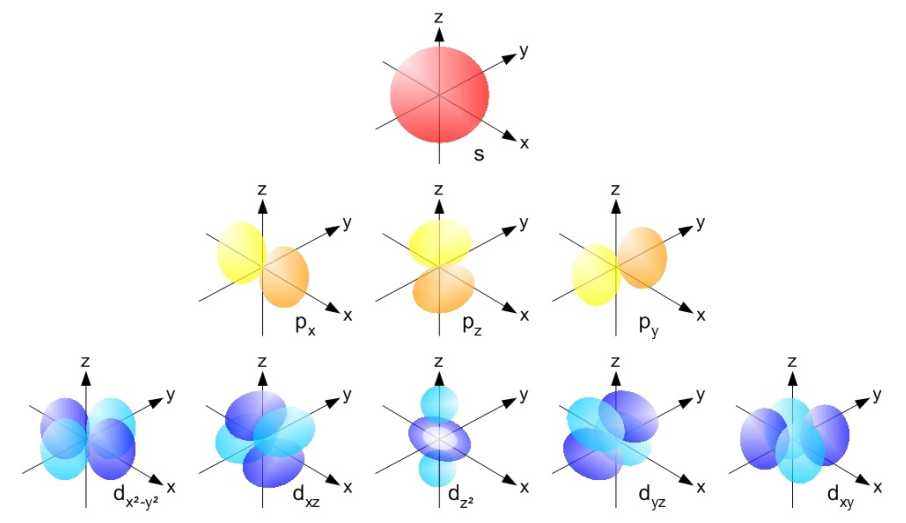
\includegraphics[width=6.0cm]{images/Fig_1_1_4_dec.png}
\centering
\end{figure}
\vspace{-\parskip}
\vspace{2mm}
\par
6. $N_S = 2S^2+3S+1$; $N_A= 2S^2+S$.\par
7. Связь базисов $\ket{L M_L}$ и $\ket{L_1 m_{L_1}}\ket{L_2 m_{L_2}}$:\par
\vspace{-\parskip+1mm}
$\ket{2\pm2}=\ket{1\pm1}\!\ket{1\pm1};$\quad $\ket{2\pm1} = \frac{1}{\sqrt2}(\ket{10}\!\ket{1\pm1} + \ket{1\pm1}\!\ket{10});$\par
\vspace{-\parskip+1mm}
$\ket{20} = \frac{1}{\sqrt6}(\ket{1-1}\!\ket{11} + 2\ket{10}\!\ket{10}+\ket{11}\!\ket{1-1});$\par
\vspace{-\parskip+1mm}
$\ket{1\pm1} = \frac{1}{\sqrt2}(\ket{10}\!\ket{1\pm1} - \ket{1\pm1}\!\ket{10});$\quad$\ket{10} = \frac{1}{\sqrt2}(\ket{1-1}\!\ket{11} - \ket{11}\!\ket{1-1});$\par
\vspace{-\parskip+1mm}
$\ket{00} = \frac{1}{\sqrt3}(\ket{1-1}\!\ket{11} - \ket{10}\!\ket{10}+\ket{11}\!\ket{1-1}).$\par
\vspace{-\parskip+1mm}
Вероятности $W_J$ обнаружить различные значения полного момента $J$: $W_{2} = 2/3$, $W_{1} = 0$, $W_{0} = 1/3$.
%\hspace{\fill}
\par
8. $2L_2+1$.\par
9. Количество состояний с определенными проекциями полного момента для~системы из $N$ электронов подчиняется биномиальному распределению. Любой возможный полный спин системы $K$ имеет нулевую проекцию. Всего нулевых проекций $C_{N}^{\,N/2}$. Любой возможный полный спин системы $K>0$ имеет проекцию равную 1. Всего единичных проекций $C_{N}^{\,(N+2)/2}$. Тогда $K=0$ в данной системе встретится $C_{N}^{\,N/2} - C_{N}^{\,(N+2)/2}$ раз. В случае нечетного $N$ задача решается аналогично, только минимальный возможный полный спин системы равен 1/2, то есть каждый полный спин $K$ имеет проекцию $1/2$. \par
10. $\widehat{S}_-=\begin{pmatrix}
0 & 0 & 0 & 0 & 0 & 0 \\
\sqrt{5} & 0 & 0 & 0 & 0 & 0\\
0 & 2\sqrt{2} & 0 & 0 & 0 & 0\\
0 & 0 & 3 & 0 & 0 & 0\\
0 & 0 & 0 & 2\sqrt{2} & 0 & 0\\
0 & 0 & 0 & 0 & \sqrt{5} & 0\\
\end{pmatrix}$
\par
11. $(\vec{S}_1,\vec{S}_2)=\frac{1}{2}( J^2 - S_1^2-S_2^2)$, где $J$ – полный спин системы. Средние значения равны $1/4$ и $-3/4$ для триплетного и синглетного состояния, соответственно.\par
12. $n^2.$\par
13. Задача 1 контрольной работы 1 осеннего семестра 2023/2024 учебного года. Систему можно обнаружить в состояниях с полным моментом $J_1=S_1+S_2$ и $J_2=S_1+S_2-1$ с вероятностями $W_1=\frac{S_1}{S_1+S_2}$; $W_2=\frac{S_2}{S_1+S_2}$. Среднее значение квадрата полного момента равно $\braket{S^2}=(S_1+S_2 )^2+S_1-S_2$.
\par
14. $3S^2-4n^2+3S+1$, если $S$ и $n$ – целые числа.\par
15. Для данного состояния могут реализоваться два значения полного спина $2N$ и $2N-1$ с вероятностями $W_{N}=\frac{1}{2N}$; $W_{N-1}=\frac{2N-1}{2N}$.\par
16. $\ket{\frac{3}{2}\,\frac{3}{2}}=\alpha\alpha\alpha$;\hspace{\fill}
$\ket{\frac{3}{2}\,\frac{1}{2}}=\frac{1}{\sqrt3}( \beta\alpha\alpha+\alpha\beta\alpha +\alpha\alpha\beta);$\hspace{\fill}$\ket{\frac{3}{2}\,-\!\frac{1}{2}}=\frac{1}{\sqrt3}( \alpha\beta\beta +\beta\alpha\beta +\beta\beta\alpha);$\par
\vspace{-\parskip+1mm}
$\ket{\frac{3}{2}\,-\!\frac{3}{2}}=\beta\beta\beta$. \hspace{\fill} $\ket{\frac{1}{2}\,\frac{1}{2}}_1 = \frac{1}{\sqrt2}( \beta\alpha\alpha-\alpha\beta\alpha);$ \hspace{\fill} $\ket{\frac{1}{2}\,\frac{1}{2}}_2 = \frac{1}{\sqrt6}( \beta\alpha\alpha+\alpha\beta\alpha -2\alpha\alpha\beta)$;\par
\vspace{-\parskip+1mm}
$\ket{\frac{1}{2}\,-\!\frac{1}{2}}_1 = \frac{1}{\sqrt2}( \alpha\beta\beta-\beta\alpha\beta);$ \quad $\ket{\frac{1}{2}\,-\!\frac{1}{2}}_2 = \frac{1}{\sqrt6}( \alpha\beta\beta+\beta\alpha\beta -2\beta\beta\alpha)$.
\par
17. Количество состояний с определенными проекциями полного момента для~системы из $N$ электронов подчиняется биномиальному распределению. Для~проекции $M =N/2-k$ количество состояний равно $C_{N}^{\,N/2-M}=C_{N}^{\,k}$. Альтернативно можно воспользоваться треугольником Паскаля:\par
\vspace{0.7mm}
\Longstack[l]{
%N=0\\
N=1\\
N=2\\
N=3\\
N=4\\
N=5\z \\
%M\qquad\ \\
}\hspace{\fill}
\Longstack{
1\x 1\\
1\x 2\x 1\\
1\x 3\x 3\x 1\\
1\x 4\x 6\x 4\x 1\\
1\x 5\y\, 10\z\, 10\y\, 5\quad\,\,\,\,\, 1\\
}\quad\quad
\Longstack{
1\x 1 \x 1\\
1\x 2\x 3\x 2\x 1\\
1\x 3\x 6\x 7\x 6\x 3\x 1\\
1\x 4\y 10\z 16\z 19\z 16\z 10\y 4\x 1\\
1\x 5\y 15\z 30\z 45\z 51\z 45\z 30\z 15\y 5\x 1\\
}
\vspace{-\parskip}
\\
Система частиц с моментом $\geq1$ описывается мультиномиальным распределением. Его можно визуализировать с использованием обобщенного треугольника Паскаля, который для момента 1 приведен выше. Количество состояний с~определенными проекциями полного момента будет определяться мультиномиальными коэффициентами.\par
18. Задача 2 контрольной работы 1 осеннего семестра 2024/2025 учебного года. (1) Полная волновая функция – антисимметрична: $\frac{1}{\sqrt{2}}(\phi_1\phi_2-\phi_2\phi_1)\ket{T_{0,\,\pm1}};$ $\frac{1}{\sqrt{2}}(\phi_1\phi_2+\phi_2\phi_1)\ket{S_{0}},$ где $\ket{T_{0,\,\pm1}}$ и $\ket{S_{0}}$ – триплетные и синглетные спиновые волновые функции, соответственно, $\phi_1, \phi_2$ – орбитальные волновые функции. (2)~Полную волновую функцию можно не антисимметризовать: $\phi_1\phi_2\alpha\alpha$, $\phi_1\phi_2\alpha\beta$, $\phi_1\phi_2\beta\alpha$, $\phi_1\phi_2\beta\beta$. (3) Полная волновая функция должна быть симметрична относительно перестановки, тогда: $\frac{1}{\sqrt{2}}(\phi_1\phi_2+\phi_2\phi_1)\ket{2\,M_S};$ $\frac{1}{\sqrt{2}}(\phi_1\phi_2-\phi_2\phi_1)\ket{1\,M_S};$ $\frac{1}{\sqrt{2}}(\phi_1\phi_2+\phi_2\phi_1)\ket{0\,0},$ где $\ket{2\, M_S}$, $\ket{1\, M_S}$, $\ket{0\, M_S}$ – соответствующие спиновые волновые функции для полного спина $S=2,1,0$, см. задачу 1.7. Частицы можно считать различимыми, если они расположены на большом расстоянии друг от~друга, по~сравнению с их областью делокализации, то есть если их волновые функции не перекрываются.\par
19. Матричные элементы равны 24, $-3$, $-9$, соответственно.\par
20. Задачу можно решить прямым расчетом интеграла $\braket{\psi|{S}^2|\psi}$, используя равенства ${S}^2 = (\vec{S},\,\vec{S})=S_{z}S_{z}+S_{y}S_{y}+S_{x}S_{x}$, $S_x=(S_+ + S_-)/2$, $S_y=(S_+ - S_-)/2i$. Расчет дает $\braket{{S}^2} = n^2 - nN + \frac{1}{4}N(N+2)$.\par
\newpage

\subsection{Термы многоэлектронных атомов}
1. В пределе LS связи для данной электронной конфигурации реализуются термы: $^4S$, $^2D$, $^2P$. При учете слабого спин-орбитального взаимодействия возникают мультиплеты:  $^4S_{\frac32}$, $^2D_{\frac52,\,\,\frac32}$, $^2P_{\frac32,\,\,\frac12}$.\par
2. Основной терм $^4I$, основной мультилет $^4I_{\frac92}$.\par
3. Термы: $1 \times \,^2G$, $ 3 \times \,^2F$, $ 5 \times \,^2D$, $ 6 \times \,^2P$, $ 2 \times \,^2S$, $1 \times \,^4F$, $ 3 \times \,^4D$, $ 3 \times \,^4P$, $ 2 \times \,^4S$, $1 \times \, ^6P$. Мультиплеты: $1 \times \,^2G_{\frac92,\,\frac72}$, $ 3 \times \,^2F_{\frac72,\,\frac52}$, $ 5 \times \,^2D_{\frac52,\,\frac32}$, $ 6 \times \,^2P_{\frac32,\,\frac12}$, $ 2 \times \,^2S_{\frac12}$, $1 \times \,^4F_{\frac92,\,\frac72,\,\frac52,\,\frac32}$, \par
\vspace{-\parskip+1.3mm}
$ 3 \times \,^4D_{\frac72,\,\frac52,\,\frac32,\,\frac12}$, $ 3 \times \,^4P_{\frac52,\,\frac32,\,\frac12}$, $ 2 \times \,^4S_{\frac32}$, $1 \times \,^6P_{\frac72,\,\frac52,\,\frac32}$.\par
4. Основной терм $^{n+1}\left[\frac n2 (2l-n+1)\right]$.\par
5. Основной терм $^{3}\left[ 2l+1 \right]$. Общее число термов $N_{\Sigma}=2l+1$. Триплетных термов $N_{\text{T}}=l$. Синглетных термов $N_{\text{S}}=l+1$.\par
\begin{wrapfigure}{r}{38mm} %this figure will be at the right
    \centering
    \vspace{-2mm}
    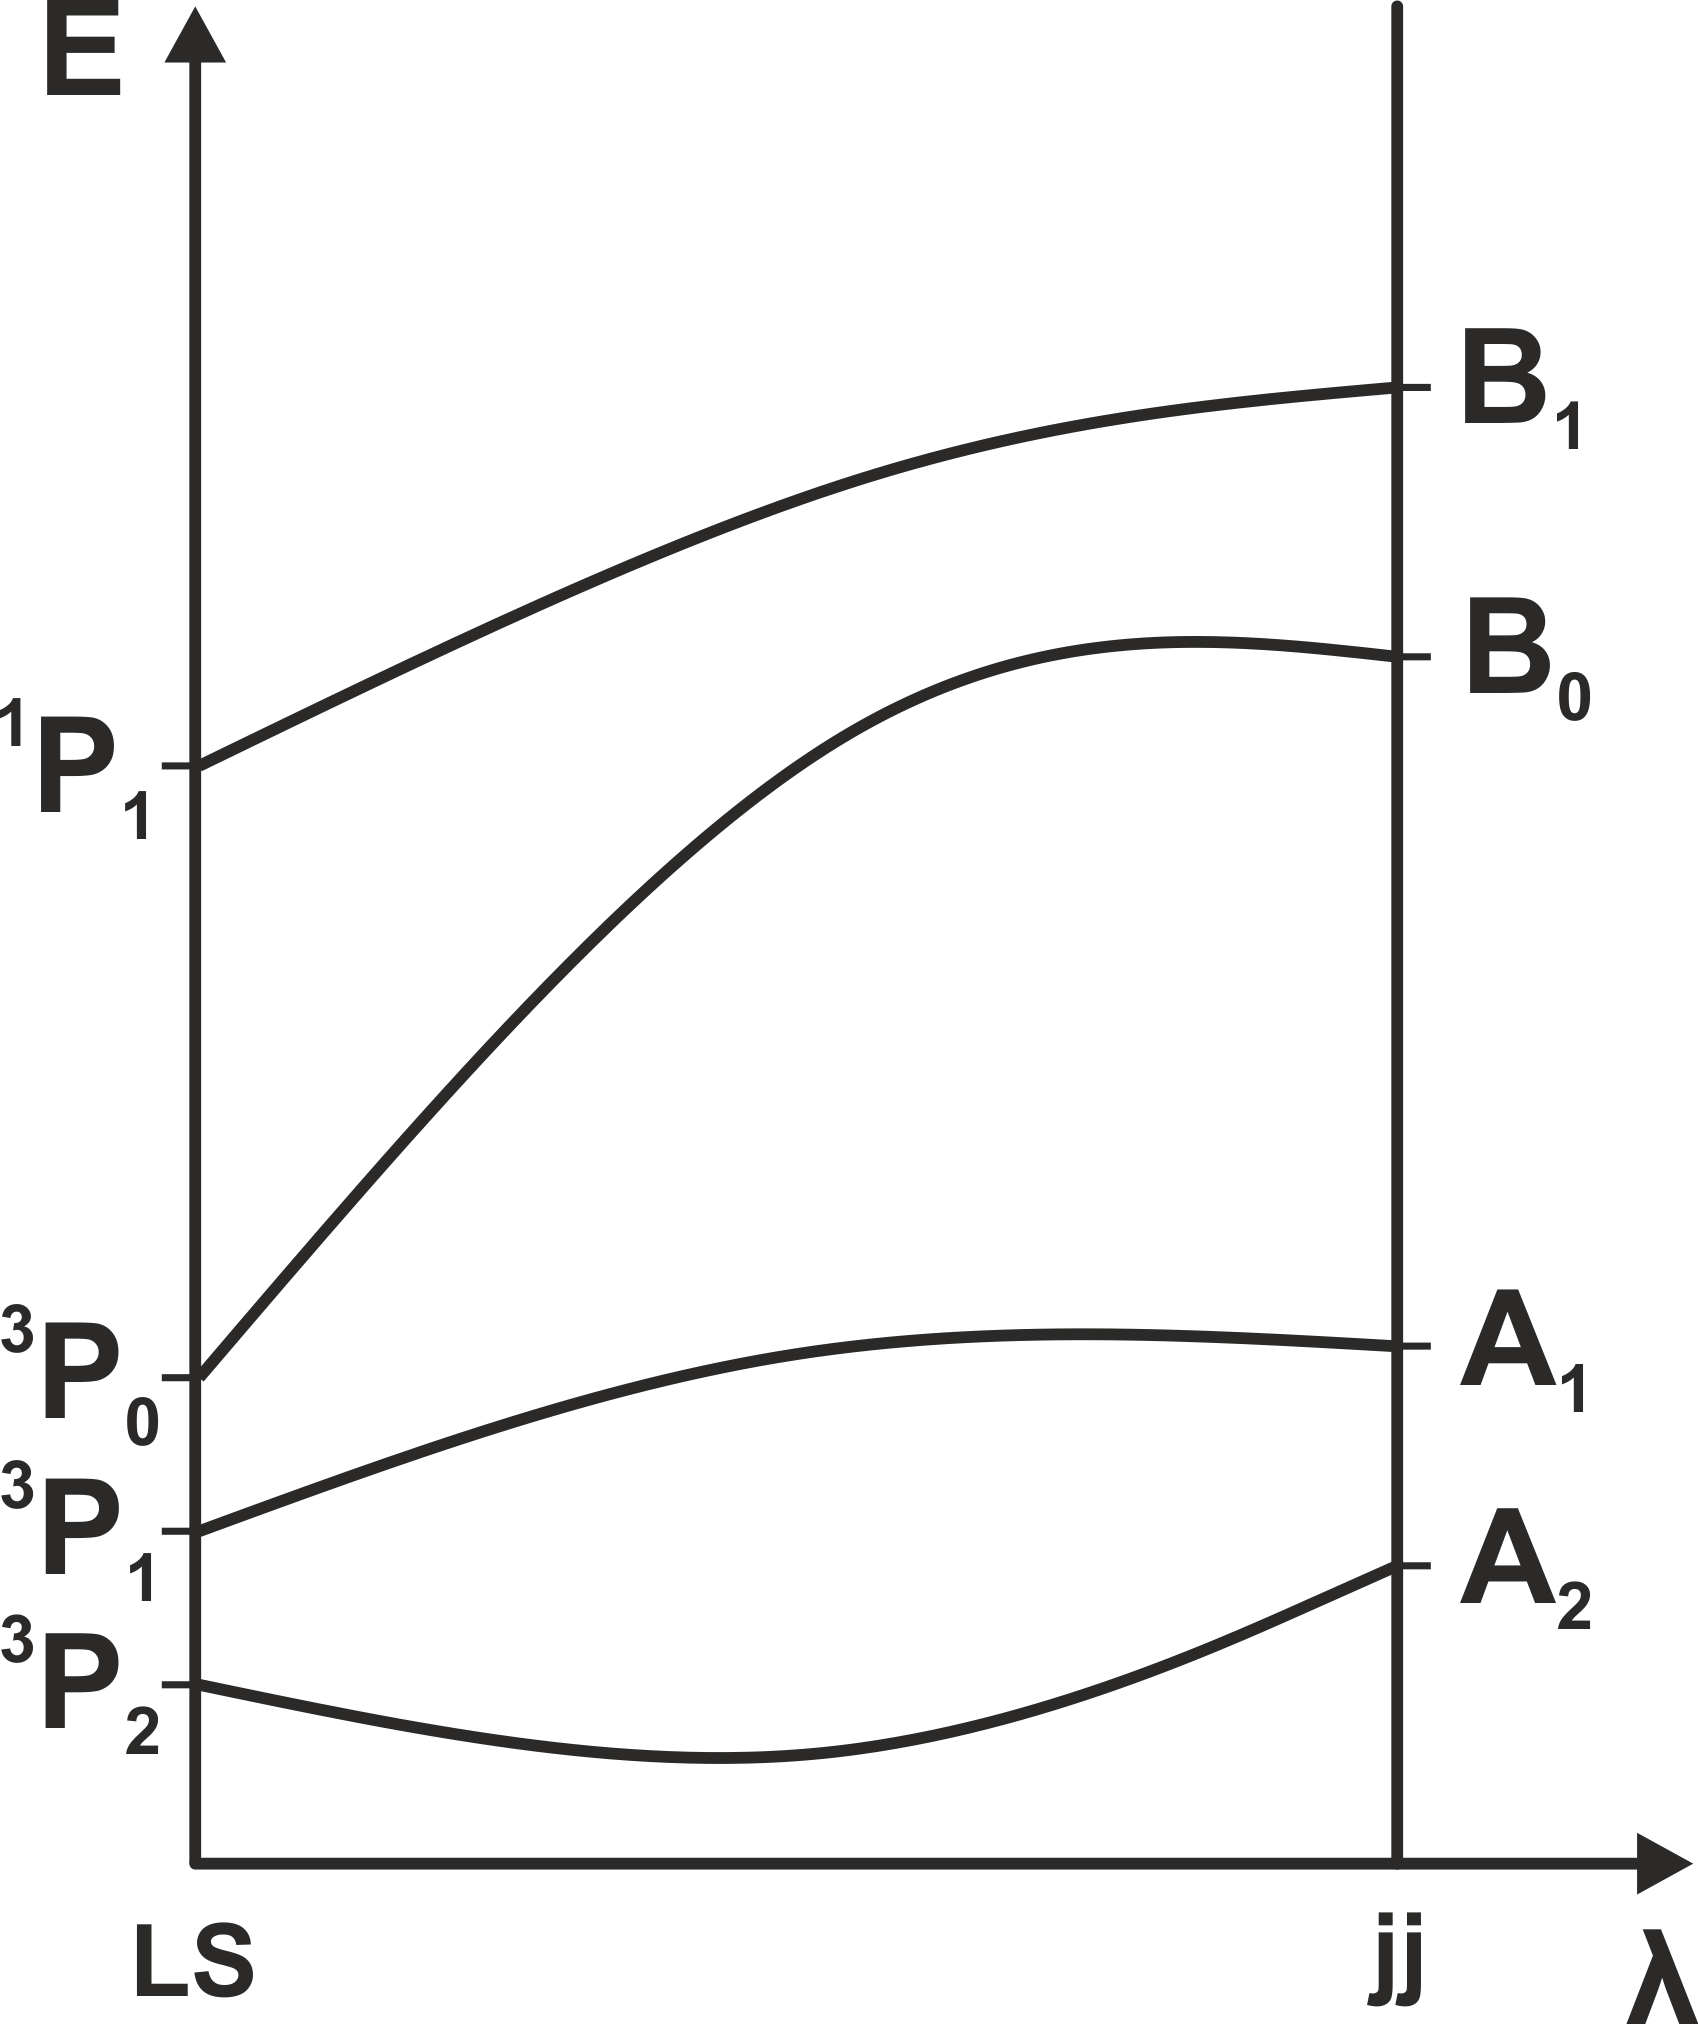
\includegraphics[width=30mm]{images/Fig_1_2_6_dec.png}
    \vspace{-3mm}
\end{wrapfigure}
6. Мультиплеты данной конфигурации в пределе LS\hspace{\fill}связи:\hspace{\fill}$^3P_{2,\,1,\,0}$,\hspace{\fill}$^3P_{1}$;\hspace{\fill}в\hspace{\fill}пределе\hspace{\fill}jj\hspace{\fill}связи:\par
\vspace{-\parskip+1mm}
$\Big( \frac32\,\,\frac32\,\,\frac32\,\,\frac12\,\,\frac12\,\,\frac12 \Big)_{2,\,1}$,\hspace{\fill}$\Big( \frac32\,\,\frac32\,\,\frac32\,\,\frac32\,\,\frac12\,\,\frac12 \Big)_{1,\,0}$.\hspace{\fill}Мультиплеты\par
\vspace{-\parskip+1mm}
коррелируют по величине полного момента $J$. Состояния с одинаковой симметрией (с одинаковым $J$) пересекаться не могут. Качественная корреляционная диаграмма приведена на рисунке. Реализующиеся состояния для случайя jj связи для удобства обозначены $A_{2,\,1}$ и $B_{1,\,0}$. При решении задачи можно также использовать эквивалентную электронную конфигурацию $p^1s^1$, если в ней корректно учесть изменение знака эффективной константы спин-орбитального взаимодействия $\lambda$, при неизменных знаках одноэлектронных констант спин-орбитального взаимодействия $\xi_i$. \par
7. Функция принадлежит электронной конфигурации $n_1p^1n_2d^1$ и терму $^3F$.\par
8. В пределе jj связи для данной электронной конфигурации реализуются термы: $\Big( \frac32\,\,\frac32\,\,\frac32 \Big)_{\frac32}$, $\Big( \frac12\,\,\frac32\,\,\frac32 \Big)_{\frac52,\,\frac32,\,\frac12}$, $\Big( \frac12\,\,\frac12\,\,\frac32 \Big)_{\frac32}$. Последний терм является основным.\par
9. В данном случае термы можно найти используя антисимметричность полной волновой функции относительно перестановки тождественных электронов. Полная волновая функция представляет собой произведение спиновой и орбитальной части, симметрия каждой из которых чередуется начиная с~симметричного поведения для максимального момента. Итого реализуются термы: $^1N$, $^1L$, $^1I$, $^1G$, $^1D$, $^1S$, $^3M$, $^3K$, $^3H$, $^3F$, $^3P$.\par
10. Задача 1 дифференциального зачета осеннего семестра 2023/2024 учебного года. Используя правило интервалов Ланде можно определить 4 величины $\lambda$~равные $-104$ см$^{-1}$, $-96$ см$^{-1}$, $-92$ см$^{-1}$, $-90$ см$^{-1}$. Отсюда $\overline \lambda = -95,5$ см$^{-1}$.\par
11. Основной терм $^4S$. Волновые функции, обозначаемые $\ket{L\,M_L;\,S\,M_S}$, являются произведением орбитальной и спиновой части. Орбитальная часть имеет вид: $\psi_0=\frac{1}{\sqrt6}(\phi_1\phi_0\phi_{-1} + \phi_0\phi_{-1}\phi_{1} + \phi_{-1}\phi_1\phi_{0} - \phi_{-1}\phi_0\phi_{1} - \phi_1\phi_{-1}\phi_{0} - \phi_0\phi_1\phi_{-1} )$, где $\phi_1 = \textit{Y}_{11}$, $\phi_0 = \textit{Y}_{10}$, $\phi_{-1} = \textit{Y}_{1-1}$. Спиновая часть, см. также задачу 1.1.16, имеет вид: $\xi_{\frac32}=\alpha \alpha \alpha$, \par
\vspace{-\parskip+0.8mm}
$\xi_{\frac12}=\frac{1}{\sqrt3} (\beta \alpha \alpha + \alpha \beta \alpha + \alpha \alpha \beta )$,\hspace{\fill}$\xi_{-\frac12}=\frac{1}{\sqrt3} (\alpha \beta \beta + \beta \alpha \beta + \beta \beta \alpha )$,\hspace{\fill}$\xi_{-\frac32}=\beta \beta \beta$.\hspace{\fill}Волновые \par
\vspace{-\parskip+1.2mm}
функции\hspace{\fill}основного\hspace{\fill}терма\hspace{\fill}$\ket{0\,0;\,\frac32\,\frac32}=\psi_0 \xi_{\frac32}$,\hspace{\fill}$\ket{0\,0;\,\frac32\,\frac12}=\psi_0 \xi_{\frac12}$, $\ket{0\,0;\,\frac32\,-\!\frac12}=\psi_0 \xi_{-\frac12}$, \par
\vspace{-\parskip+1mm}
$\ket{0\,0;\,\frac32\,-\!\frac32}=\psi_0 \xi_{-\frac32}$.\par
12. Например, электронные конфигурации $g^8$ и $g^{10}$.\par
13. Основной терм $^{m+1}\left[\frac m2 (2l-m+1)\right]$. Кратность вырождения данного равна $(2S+1)(2L+1)$. Подставляя в это выражение $S$ и $L$ и  дифференцируя по $m$, можно найти значение параметра $m$, соответствующее максимальному вырождению. Оно равно $m=\frac{2l+\sqrt{4l^2 +6l+6}}{3} \rightarrow \frac{4l}{3}$, если $l \rightarrow \infty$.\par
14. Чтобы определить количество термов с максимальным полным спином, необходимо посчитать сколькими способами можно составить микросостояние с проекцией полного орбитального момента $M_L=0$ и проекцией полного спина $M_S=3/2$, с учетом принципа Паули. Перебирая все подходящие микросостояния и суммируя получившиеся арифметические прогрессии, получим искомое количество термов $N_{\Sigma}=\frac{l^2}{2}$, если $l=2k$, где $k=0,1,2,\ldots$; $N_{\Sigma}=\frac{l^2+1}{2}$, если $l=2k+1$, где $k=0,1,2,\ldots$.\par
15. Задача 3 контрольной работы 1 осеннего семестра 2022/2023 учебного года. Основной терм $^{n+2 }\left[\frac n2 (2l-n+1)\right]$.\par
16. Количество мультиплетов для частных случаев jj и LS связи одинаково, при этом его намного проще посчитать для LS связи. Используя антисимметричность полной волновой функции относительно перестановки тождественных электронов, см. задачу 1.2.9, можно определить все термы и мультиплеты электронной конфигурации $l^2$. Число состояний с определенным значением $J$ равно числу мультиплетов $N_J=4l+1$.\par
17. Задача 4 контрольной работы 1 осеннего семестра 2023/2024 учебного года. Среднюю энергию всех мультиплетов, возникающих из терма $^{2S+1}L$, можно определить по выражению для $L\geq S$:
\begin{equation*}
\begin{aligned}
&\overline E=\sum_{J=L-S}^{L+S} \dfrac{g_JE_J}{(2S+1)(2L+1)} = \ldots = E_0,\hspace{41mm}
\end{aligned}
\end{equation*}
где $g_J=(2J+1)$ – кратность вырождения мультиплета, $E_J$~– его энергия. Энергия мультиплета равна $E_J=E_0+\lambda/2 ( J(J+1)-L(L+1)-S(S+1) )=E_0+E_{LS}$, где $E_0$~–~энергия терма. Суммарная дополнительная энергия всех мультиплетов, вызванная спин-орбитальным взаимодействием, может быть определена используя следующую сумму:
\begin{equation*}
\begin{aligned}
&E_{\Sigma}=\sum_{J=L-S}^{L+S} g_JE_{LS} = \ldots = 0.\hspace{55mm}
\end{aligned}
\end{equation*}
Таким образом, средняя энергия всех мультиплетов, возникающих из некоторого терма $^{2S+1}L$, равна энергии этого терма. Задача имеет альтернативное решение, использующее инвариантность следа матрицы относительно смены базиса.
\par
18. Задача 1 контрольной работы 1 осеннего семестра 2024/2025 учебного года. Реализуются термы: ${^2}\Big[ \frac{7}{2}\Big]_{4,3}$;\, ${^2}\Big[ \frac{5}{2}\Big]_{3,2}$;\, ${^2}\Big[ \frac{3}{2}\Big]_{2,1}$;\, ${^2}\Big[ \frac12\Big]_{1,0}$;\, ${^2}\Big[ \frac{5}{2}\Big]_{3,2}$;\, ${^2}\Big[ \frac{3}{2}\Big]_{2,1}.$\par
19. При расчете нормировочного множителя возникает интеграл, который можно посчитать, например, методом дифференцирования по параметру. Итого $A=\frac{(2\xi)^n}{a_0} \sqrt{\frac{2 \xi}{a_0 (2n)!}}$. Безразмерный радиус, соответствующий максимуму плотности вероятности, можно найти из уравнения $\sfrac{\text{d} R_n^2(r)\,r^2 }{\text{d}r} = 0$. Он равен $r_{max}=\sfrac{a_0(n^*)^2}{(Z-s)}$. Значения параметров $n^*$ и $s$ для атома железа можно определить по специальным правилам, изложенным, например, в главе 2.4 учебного пособия [3], см.~список литературы. Размер атома железа ($3d^64s^2$) можно оценить по~внешней $4s$ оболочке. Для $4s$ электрона $s = 22,25$, $n^*=3,7$. Кроме того, $a_0=0,529\,\,\text{\r{A}}$ и $Z_{\text{Fe}}=26$, тогда  $r_{\text{Fe}}=1,93\,\,\text{\r{A}}$.

\par
\newpage

\subsection{Дипольные переходы между термами}
1. Задача 2 контрольной работы 1 осеннего семестра 2023/2024 учебного года. Не равна нулю только $d_z$ компонента вектора $\vec d$. Она равна $\sfrac{3ea_0}{Z}$, где $a_0$ – радиус Бора, $Z$ – заряд ядра. Величина электрического дипольного момента перехода совпадает с $d_z$.\par
2. Задача 3 контрольной работы 1 осеннего семестра 2023/2024 учебного года. Основной мультиплет $^3H_4$. Электические дипольные переходы возможны в~мультиплеты $^3G_3$, $^3F_{3,\,2}$, $^3D_{3,\,2,\,1}$. Возбужденная электронная конфигурация должна быть четной.\par
3. Задача 5 контрольной работы 1 осеннего семестра 2024/2025 учебного года.  Полное количество термов 47. Основной терм $^5I$. Переход возможен в любую нечетную электронную конфигурацию, например, $6s^14f^46p^1$.\par
4. Задача 3 контрольной работы 1 осеннего семестра 2024/2025 учебного года. Всего 18 переходов. Условию удовлетворяют переходы $^3P\, \rightarrow\, ^3P$ и переходы $^3P\, \rightarrow\, ^3D$. Всего их 7 штук.\par
5. Задача 5 контрольной работы 1 осеннего семестра 2023/2024 учебного года. Серия А относится к переходу (1). Серия B относится к переходу (2). Серия C~относится к переходу (1).   \\
\newpage

\subsection{Многоэлектронный атом во внешних полях}
1. \par
2. \par
3. \par
4. Задача 4 контрольной работы 1 осеннего семестра 2024/2025 учебного года. Эффективная константа спин-орбитального взаимодействия $\lambda$ равна 0,12 см$^{-1}$, индукция магнитного поля $B$ равна 2,014 Тл.\par
5. \par
6. \par
7. \par
8. \par
9. \par
10. \par
11. \par
12. \par
13. \par
14. \par
15. \par
\newpage

\subsection{Правила Вигнера-Витмера}
1. Независимых волновых функций: 1 ($^1\Sigma^-$), 3 ($\,^3\Sigma^+$), 6 ($\,^3\Pi$), 2 ($^1\Phi$), 12~($^6\Delta$). \par
2.  $^{6,4,2}\Pi$,  $^{6,4,2}\Sigma^+$.\par
3. (1) $^3\Delta_u$, $^1\Delta_g$, $^{3,1}\Pi_g$, $^{3,1}\Pi_u$, $2 \times ^{3}\Sigma_u^+$, $^3\Sigma^-_g$, $2 \times ^{1}\Sigma_g^+$, $^{1}\Sigma_u^-$; (2) $^{3,1}\Pi_g$, $^{3,1}\Pi_u$, $^{3,1}\Sigma^-_g$, $^{3,1}\Sigma^-_u$; (3)~$^3\Pi_g$, $^3\Pi_u$, $^3\Sigma^-_g$, $^3\Sigma^-_u$.\par
4. $(2S_2+1)(2L_2+1)(L_1+1).$\par
5.  $^{5}\Sigma^+$, $3 \times ^{3}\Sigma^+$, $2 \times ^{1}\Sigma^+$.\par
6. Задача 2 контрольной работы 1 осеннего семестра 2021/2022 учебного года. Термы: $^3\Pi$, $^3\Sigma^-$. Основного состояния молекулы BeO получиться не может. Для образования BeO в основном электронном состоянии нужно, например, возбужденное состояние атома бериллия $^3P$, соответствующее электронной конфигурации $2s^12p^1$.\par
7. Задача 2 контрольной работы 2 осеннего семестра 2024/2025 учебного года. Реакция протекает по гомолитическому механизму.\par
8. Образование CO в основном состоянии в этом случае возможно.\par
9. $^1\Delta_g$, $^1\Pi_g$, $^1\Pi_u$, $2 \times ^1\Sigma^+_g$, $^1\Sigma^-_u$.\par
10. $1 + LS + S + L(2 + L + 2(1 + L)S)$.\par
\newpage

\subsection{Электронное строение двухатомных молекул}
1. \par
2. \par
3. \par
4. \par
5. \par
6. \par
7. \par
8. \par
\newpage

\subsection{Электронное строение многоатомных молекул}
1. Задача 2 контрольной работы 2 осеннего семестра 2022/2023 учебного года. Основное состаяние $\text{BeH}_2^{+\boldsymbol{\cdot}}$ имеет электронную конфигурацию $(\sigma_g^+)^2 (\sigma_u^+)^1$, основной терм $^2\Sigma_u^+$. Первое возбужденное состояние соответствует конфигурации $(\sigma_g^+)^1 (\sigma_u^+)^2$ и терму $^2\Sigma_g^+$. Переход между термами разрешен в $\pi$ поляризации.\par
2. Группа симметрии данной системы $D_{3h}$. Симметрия и энергия $E_i$ молекулярных орбиталей: $1a_1'$ $E_1=\alpha+(1+\sqrt3)\beta$, $e'$ $E_{2,3}=\alpha+\beta$, $1a_2''$ $E_4=\alpha+(\sqrt3-1)\beta$, $2a_1'$~$E_4=\alpha-(\sqrt3-1)\beta$, $e''$ $E_{6,7}=\alpha-\beta$, $2a_2''$~$E_8=\alpha-(1+\sqrt3)\beta$. Основной терм $^1A_1'$, разрешены 5 электрических дипольных переходов в термы $^1A_2''$ $(1a_2'' \rightarrow 2a_1')$, $^1A_2''$ $(e' \rightarrow e'')$, $^1A_2''$ $(1a_1' \rightarrow 2a_2'')$, $^1E'$ $(2a_2'' \rightarrow e'')$, $^1E'$~$(e' \rightarrow 2a_1')$. В скобках указаны переходы между одноэлектронными молекулярными орбиталями.\par
3. Поскольку расстояние между  $2s$ и $2p$ орбиталями атома кислорода достаточно велико, при решении можно рассматривать только $2p$ атомные орбитали. Для трех атомов кислорода шесть из девяти $2p$ орбиталей образуют три дважды вырожденные молекулярные орбитали (МО) $\pi$-типа, расположенные аналогично $\pi$-системе аллильного радикала. Оставшиеся три $2p$ орбитали взаимодействуют по $\sigma$-типу и образуют три невырожденные МО, причем уровень $\alpha$ оказывается трехкратно вырожденным (две $\pi$ и одна $\sigma$ МО). Всего в молекуле 12 электронов (три атома $2p^4$), тогда электронная конфигурация полностью заполнена и основной терм линейного озона $^1\Sigma_g^+$. \par
4. Задача 1 контрольной работы 2 осеннего семестра 2023/2024 учебного года. Группа симметрии данной молекулы $C_{2v}$. Симметрия и энергия молекулярных орбиталей: $1b_2$ $E_1=\alpha+2,11\beta$, $2b_2$ $E_2=\alpha+\beta$, $1a_2$ $E_3=\alpha+0,62\beta$, $3b_2$ $E_4=\alpha-0,25\beta$, $2a_2$ $E_5=\alpha-1,62\beta$, $4b_2$ $E_6=\alpha-1,86\beta$. Фульвен обладает дипольным моментом в результате переноса заряда, так как при этом циклопентадиенильный фрагмент молекулы становится ароматической системой.\par
5. Задача 5 дифференциального зачета осеннего семестра 2023/2024 учебного года. Группа симметрии данной молекулы $T_{d}$. Качественный порядок молекулярных орбиталей (от более отрицательной энергии к менее отрицательной) $1a_1$, $1t_2$, $2a_1$, $2t_2$. Основной терм нейтральной молекулы $^1A_1$, катион-радикала $^2T_2$, анион-радикала $^2A_1$. Наибольшей устойчивостью обладает нейтральная молекула.\par
6. Группа симметрии данной системы $D_{4h}$. Симметрия и энергия молекулярных орбиталей:\hspace{\fill}$1a_{2u}$\hspace{\fill}$E_1=\alpha+(1+\sqrt5)\beta$,\hspace{\fill}$e_g$\hspace{\fill}$E_{2,3}=\alpha$,\hspace{\fill}$2a_{2u}$\hspace{\fill}$E_4=\alpha-(\sqrt5-1)\beta$,\\ $b_{1u}$ $E_5=\alpha-2\beta$. Неспаренный электрон находится на орбиталях $e_g$ симметрии, спиновая плотность $\rho_{1,2,3,4}=0,25$. Согласно теории возмущений изменение кулоновского интеграла центрального атома $\phi_5$ приводит к матричному элементу $\braket{\phi_5|V|\phi_5}=0,1\alpha$, который в первом порядке теории возмущений изменит энергии двух уровней симметрии $a_{2u}$. Изменение полной электронной энергии будет равно $\Delta E=2\braket{\psi_1(a_{2u})|V|\psi_1(a_{2u})}=3,2\alpha/(22+2\sqrt5)$.\par
7. Задача 4 контрольной работы 2 осеннего семестра 2024/2025 учебного года. Полученное с использованием теории МО ЛКАО качественное электронное строение линейной и нелинейной молекулы воды приведено на рисунке. Приведенные в условии термы соответствуют следующим электронным конфигурациям: (1) “Плоская” вода $^1\Sigma_g^+$: $(1\sigma_g^+)^2 (1\sigma_u^+)^2 (\pi_u)^4$, $^1\Pi_u$: $(1\sigma_g^+)^2 (1\sigma_u^+ )^2 (\pi_u )^3 (2\sigma_g^+ )^1$, $^1\Pi_g$: $(1\sigma_g^+)^2 (1\sigma_u^+)^1 (\pi_u )^3 (2\sigma_g^+ )^2$. (2) Вода симметрии $C_{2v}$ : $^1A_1$: $(1a_1 )^2 (1b_2 )^2 (2a_1 )^2 (b_1 )^2$, $^1B_1$: $(1a_1 )^2 (1b_2 )^2 (2a_1 )^2 (b_1 )^1  (3a_1  )^1$, $^1A_2$: $(1a_1 )^2 (1b_2 )^2 (2a_1 )^2 (b_1 )^1 (2b_2)^1$. Корреляционная диаграмма $C_{2v} \leftrightarrow D_{\infty h}$ трех первых синглетных термов также приведена на~рисунке.
\vspace{-\parskip}
\vspace{5mm}
\begin{figure}[h]
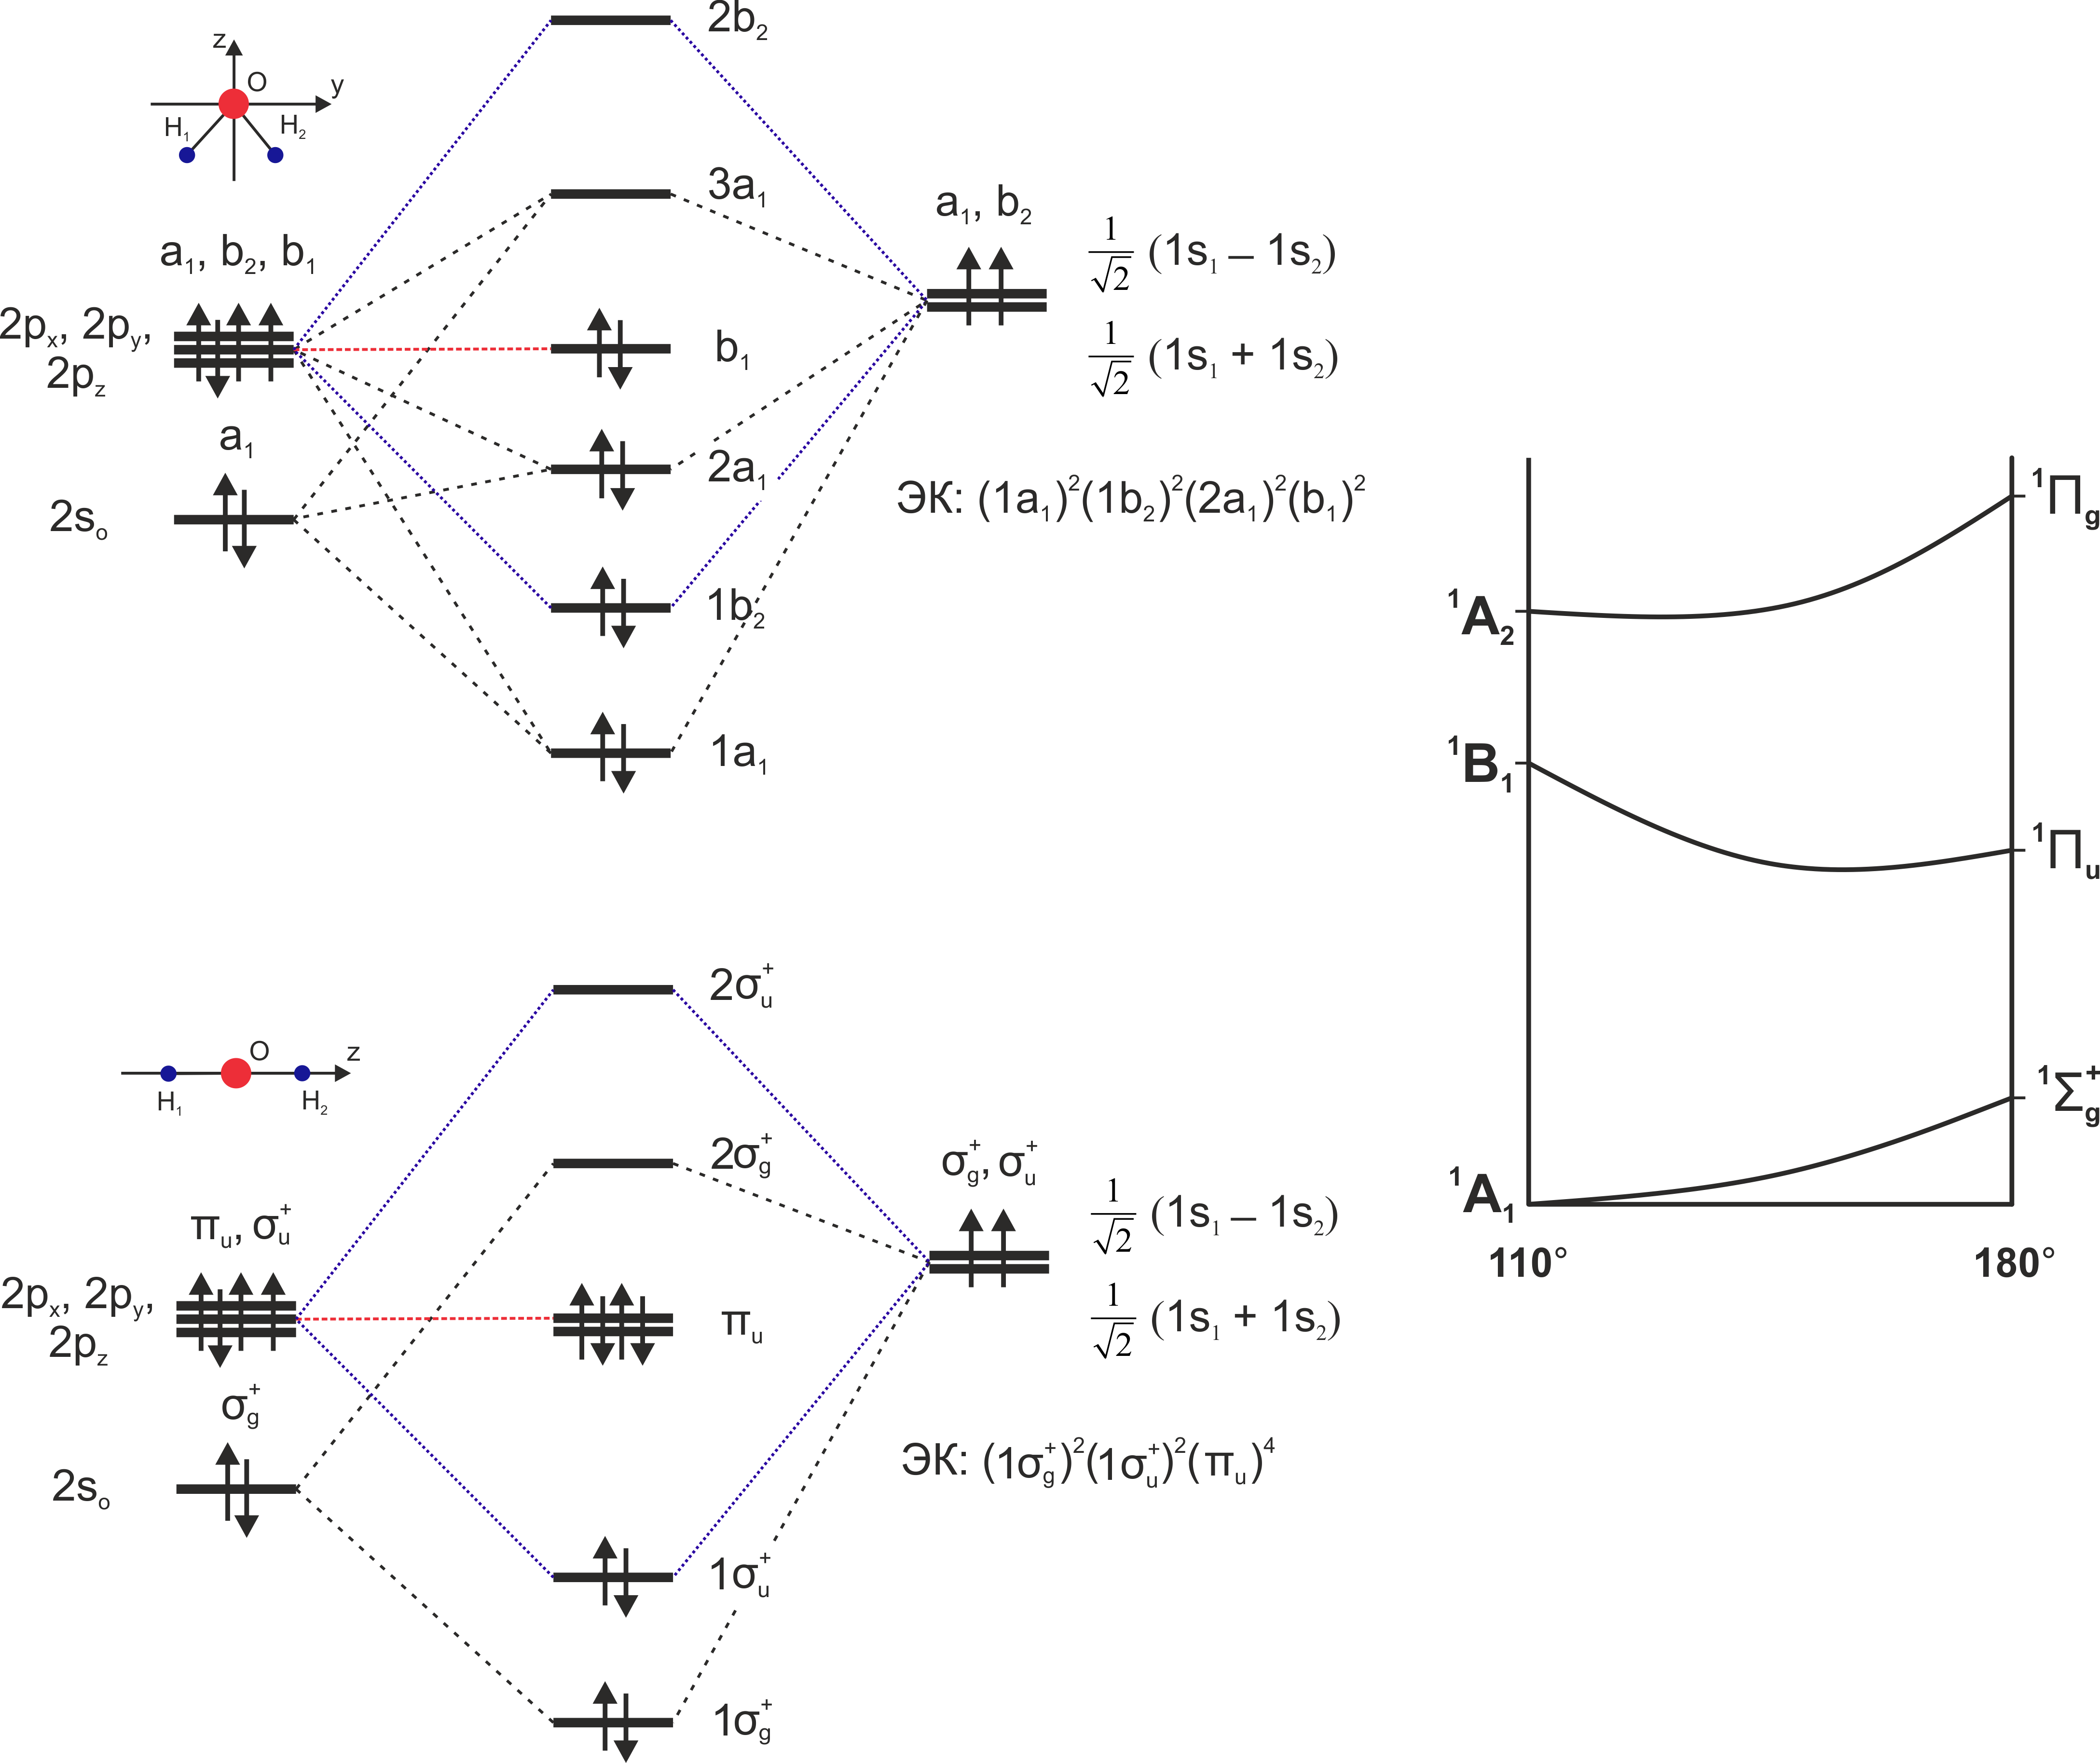
\includegraphics[width=9.4cm]{images/Fig_1_7_8_dec.png}
\centering
\end{figure}
\vspace{-\parskip}
\par
8. Задача 4 контрольной работы 2 осеннего семестра 2023/2024 учебного года. При учете интеграла перекрывания $S$ между соседними $p_z$ орбиталями для нахождения энергетических уровней и молекулярных орбиталей требуется решить следующее матричное уравнение:\par
\vspace{-\parskip}
\vspace{2mm}
\hspace{7mm}
$\begin{pmatrix}
\alpha-E & \beta-SE & 0 \\
\beta-SE & \alpha-E & \beta-SE \\
0 & \beta-SE & \alpha-E \\
\end{pmatrix}
\begin{pmatrix}
C_1 \\
C_2 \\
C_3 \\
\end{pmatrix}=0.$\par
\vspace{-\parskip}
\vspace{2mm}
Подставляя\hspace{\fill}$S=0,25$\hspace{\fill}получаем\hspace{\fill}энергии\hspace{\fill}$E_i$ равные\hspace{\fill}$\alpha$,\hspace{\fill}$1,55\alpha-2,19\beta$,\hspace{\fill}$0,74\alpha+1,04\beta$.\\ $E_{\Sigma}=2,48\alpha+2,08\beta$. Без учета $S$ энергетические уровни аллильного радикала: $\alpha$,~$\alpha-1,41\beta$, $\alpha+1,41\beta$, $E_{\Sigma}=3\alpha+2,82\beta$.\par
9. Образование молекулы ферроцена можно представить как взаимодействие катиона $\text{Fe}^{2+}$ ($3d^6$) и двух циклопентадиенильных анионов $\text{Cp}^-$. В качестве базиса орбиталей выберем $3d$ орбитали железа и $2p_z$ орбитали углерода, образующие ароматический цикл. Из-за высокой симметрии ферроцена ($D_{5d} / D_{5h}$) его можно рассматривать как квазилинейную систему в группе симметрии $D_{\infty h}$. В~этой группе $d$ орбитали железа будут иметь представления: $\Sigma_g^+$~($d_{z^2}$), $\Pi_g$~($d_{xz}, d_{yz}$), $\Delta_g$ ($d_{xy}, d_{x^2-y^2}$). Орбитали циклопентадиенила представляют собой две пятицентровые циклические системы, среди которых также найдутся комбинации с~симметрией $\Sigma_g^+$, $\Pi_g$ и $\Delta_g$. Для определенности можно считать, что взаимодействие $2p_z$ орбиталей между собой больше, чем с $d$ орбиталями железа. Итого 6~заполненных орбиталей двух Cp, далее расщепленные $d$ орбитали железа $\Delta_g$, $\Sigma_g^+$, $\Pi_g$ (в порядке увеличения энергии) и еще 4 незаполненные орбитали двух Cp. При переходе от группы $D_{\infty h}$ к $D_{5d}$ или $D_{5h}$ одномерное представление $\Sigma_g^+$  станет $А,$ двумерные $\Pi_g$ и $\Delta_g$ различными $Е$ представлениями. Таким образом качественно электронное строение можно описать конфигурацией для высокоспинового состояния Fe: $a^2(\text{Cp}) a^2(\text{Cp}) e^4(\text{Cp}) e^4(\text{Cp}) e^3(\text{Fe}) a^1(\text{Fe}) e^2(\text{Fe})$. Известно, что молекула ферроцена диамагнитна, поэтому более корректно будет рассматривать низкоспиное состояние комплекса: $a^2(\text{Cp}) a^2(\text{Cp}) e^4(\text{Cp}) e^4(\text{Cp}) e^4(\text{Fe}) a^2(\text{Fe})$. Оно соответствует полностью заполненной электронной конфигурации.\par
10. Задача 3 контрольной работы 2 осеннего семестра 2024/2025 учебного года. В данном ряду хюккелевских систем расположение энергетических уровней можно определить, например, используя теорию возмущений. Для каждого последующего $n$ происходит объединение двух одинаковых систем $n-1$, что дает поправки к энергиям $\pm \beta$. Кратность вырождения уровней при этом будет соответствовать биномиальным коэффициентам. Итого для произвольного $n$, обозначая $E_{\mu}=\alpha+\gamma_{\mu} \beta$, для заполненных МО получим для четных $n$ следующие величины кратности вырождения энергетического уровня и значения параметра $\gamma_{\mu}$:\par
\vspace{-\parskip}
\vspace{2mm}
\hspace{8mm}
\begin{tabular}{ |c|c|c|c|c| }
 КВ & $C_n^0$ & $C_n^1$ & $\ldots$ & $C_n^{n/2}$ \\ 
 $\gamma_{\mu}$ & $n$ & $n-2$ & $\ldots$ & $0$ \\  
\end{tabular}
\par
\vspace{-\parskip}
\vspace{3mm}
Для нечетных $n$:
\par
\vspace{-\parskip}
\vspace{2mm}
\hspace{8mm}
\begin{tabular}{ |c|c|c|c|c| }
 КВ & $C_n^0$ & $C_n^1$ & $\ldots$ & $C_n^{(n-1)/2}$ \\ 
 $\gamma_{\mu}$ & $n$ & $n-2$ & $\ldots$ & $1$ \\  
\end{tabular}\par
\vspace{-\parskip}
\vspace{2mm}
Свободные МО расположены симметрично, так как все рассматриваемые системы с $n > 1$ являются четными альтернантными. Полная электронная энергия определяется соответствующей суммой. Случай четного $n$:
\begin{equation*}
\begin{aligned}
& E_{\Sigma}=2^n \alpha+2\sum_{i=0}^{n/2} C_n^i (n-2i)\beta = \ldots = 2^n \alpha + (2+n)\beta C_n^{(n+2)/2}.\hspace{13mm}
\end{aligned}
\end{equation*}
Для нечетного $n$ аналогично:
\begin{equation*}
\begin{aligned}
& E_{\Sigma}= 2^n \alpha + 2\beta n C_{n-1}^{(n-1)/2} = 2^n \alpha + (1+n) \beta C_{n}^{(n+1)/2}.\hspace{27mm}
\end{aligned}
\end{equation*}
\par
\vspace{-\parskip}
%\hspace{\fill}
11. Группа симметрии молекулы $D_{3h}$. Симметрия и энергия молекулярных орбиталей: $1a_{2}''$ $E_1=\alpha+\sqrt6\beta$, $1e''$ $E_{2,3}=\alpha+\sqrt3 \beta$, $2a_{2}''$ $E_4=\alpha+\beta$, $2e''$ $E_{5,6}=\alpha+\beta$, $a_{1}''$~$E_7=\alpha$, $3a_{2}''$ $E_8=\alpha-\beta$, $3e''$ $E_{9,10}=\alpha-\beta$, $4e''$ $E_{11,12}=\alpha-\sqrt3 \beta$, $4a_{2}''$ $E_{13}=\alpha-\sqrt6 \beta$. По~теории возмущений данную молекулу можно рассматривать как циклическую систему из 12 центров и дополнительный атом в середине, что приводит к~вырожденной теории возмущений для уровней $E=\alpha$. Итоговые энергии и симметрии в первом порядке теории возмущений: $1a_{2}''$ $E_1=\alpha+2\beta$, $1e''$~$E_{2,3}=\alpha+\sqrt3 \beta$, $2a_{2}''$ $E_4=\alpha+\sqrt{3/2} \beta$, $2e''$ $E_{5,6}=\alpha+\beta$, $a_{1}''$ $E_7=\alpha$, $3e''$ $E_{8,9}=\alpha-\beta$, $3a_{2}''$ $E_{10}=\alpha-\sqrt{3/2} \beta$, $4e''$ $E_{11,12}=\alpha-\sqrt3 \beta$, $4a_{2}''$ $E_{13}=\alpha-2 \beta$. Во втором порядке теории возмущений поправка к энергии будет только для уровней с симметрией $a_2''$~с~энергией $E = \alpha \pm 2\beta$. Она равна $\Delta E^{(2)}= |\braket{\psi(a_2'')|V|\psi_{13}}|^2/(\pm 2\beta) = \pm 3/8 \beta$. Итоговые энергии МО:~$1a_{2}''$ $E_1=\alpha+2,375\beta$, $1e''$ $E_{2,3}=\alpha+\sqrt3 \beta$, $2a_{2}''$ $E_4=\alpha+\sqrt{3/2} \beta$, $2e''$ $E_{5,6}=\alpha+\beta$, $a_{1}''$~$E_7=\alpha$, $3e''$ $E_{8,9}=\alpha-\beta$, $3a_{2}''$ $E_{10}=\alpha-\sqrt{3/2} \beta$, $4e''$ $E_{11,12}=\alpha-\sqrt3 \beta$, $4a_{2}''$ $E_{13}=\alpha-2,375 \beta$.\par
12. Задача 3 контрольной работы 2 осеннего семестра 2023/2024 учебного года. Самая коротковолновая линия поглощения $\pi$-системы пентадиенильного радикала соответствует переходу между молекулярными орбиталями с~минимальной и максимальной энергией. В группе симметрии $C_{2v}$ данные орбитали соответствуют $B_2$~неприводивому представлению. Таким образом, указанный переход соответствует $\pi$~поляризации.\par
13. Задача 1 контрольной работы 2 осеннего семестра 2022/2023 учебного года. Группа симметрии молекулы $D_{2h}$. Симметрия и энергия молекулярных орбиталей: $1b_{1u}$ $E_1=\alpha+2,34\beta$, $1b_{2g}$ $E_2=\alpha+1,81\beta$, $2b_{1u}$ $E_3=\alpha+0,47\beta$, $a_{u}$ $E_4=\alpha$, $b_{3g}$~$E_5=\alpha$, $2b_{2g}$ $E_6=\alpha-0,47\beta$, $3b_{1u}$ $E_7=\alpha-1,81\beta$, $3b_{2g}$ $E_8=\alpha-2,34\beta$. Электронная конфигурация основного состояния $(1b_{1u})^2 (1b_{2g})^2 (2b_{1u})^2 (a_u)^1 (b_{3g})^1$. Основной терм $^3B_{3u}$.\par
\newpage

\subsection{Специальные хюккелевские системы}
1. Электронная конфигурация циклобутадиена $(a_{2u})^2(e_g)^2$ , если считать, что его $\pi$-система относится к группе симметрии $D_{4h}$ (ось $x$ направлена вправо между атомами углерода, ось $y$ направлена вверх между атомами углерода). Основной терм $^3A_{2g}$.\par
2. Все МО орбитали в линейной хюккелевской системе невырождены, поэтому данная система будет являться радикалом только при $n=4k+1$ и $n=4k+3$, где $k=0,1,2,\ldots$. Пусть система относится к группе симметрии $D_{\infty h}$, симметрии МО чередуются и общее количество разрешенных переходов: (1) $N=\frac{(n-1)(n+3)}{8}$, если $n=4k+1$; (2) $N=\frac{(n+1)(n+1)}{8}$, если $n=4k+3$. Число разрешенных переходов с различной энергией равно $N_{\text{E}}=N/2$, если $n = 4k+1,\,4k+3$, так как энергетические уровни расположены симметрично относительно уровня $E=\alpha$.\par
3. Используя вырожденную теорию возмущений для учета индуктивного заместителя с помощью единственного ненулевого матричного элемента оператора возмущения: $\bra{\phi_1} V \ket{\phi_1}=\xi \beta$, $\xi<0$, можно определить, что $E_{\text{ВЗМО}}=\alpha$, если $n=4k$ и $E_{\text{ВЗМО}}=\alpha+2\beta \sin{\frac{\pi}{n}}+\frac{2}{n}\xi \beta$, если $n=4k+2$.\par
4. Задача 5 дифференциального зачета осеннего семестра 2022/2023 учебного года. Описанная ситуация соответствует переходу между термами $^2B_{2g} \rightarrow\,\,^2B_{1u}$, который разрешен в $\sigma$ поляризации.\par
5. Согласно методу Хюккеля у бесконечного сопряженного полиена можно было бы ожидать появления металлической проводимости, так как энергетический зазор между заполненными и свободными молекулярными орбиталями в~такой системе должен быть близок к нулю. Расстояние между энергетическими уровнями с максимальной и минимальной энергией $\Delta E \rightarrow 4\beta$, если $n \rightarrow \infty$.  \par
6. Данная система является нечетной альтернантной. Исходя из орбитали неспаренного электрона можно определить ненулевые спиновые плотности на различных центрах: $\rho_1 = 25/56$, $\rho_2 = 7/32$, $\rho_{3,\,4,\,5,\,9,\,12} = 9/224$, $\rho_6 = 1/14$, $\rho_{7,\,10} = 1/224$,  $\rho_{8,\,11,\,13} = 1/56$. Для расчета спиновой плотности меченые центры пронумерованы в порядке сверху вниз, слева направо.\par
7. Используя общее решение для циклических систем можно определить, что порядок связи, например, между центрами 1 и $n$, равен $b_{1n}=\frac{2}{n}\sin^{-1}{\frac{\pi}{n}}$.\par
8. Формально нельзя, так как несмотря на различную симметрию, в обоих случаях в спектре поглощения будет 1 линия с энергией $2\beta$. При этом для квадратной геометрии основной триплетный терм $^3A_{2g}$ и синглетные термы $^1A_{1g}$, $^1B_{1g}$, $^1B_{2g}$, соответствующие этой же электронной конфигурации $(a_{2u})^2(e_g)^2$, имеют близкую, но неодинаковую энергию энергию, что может привести к~большему количеству линий в спектре поглощения, в сравнении с прямоугольной геометрией и соответствующей ей полностью заполененной электронной конфигурацией.\par
9. Случай $\text{H}_3^+$. Полная электронная энергия $E_{\Sigma}$: (1), (2) $2\alpha + 2\sqrt2 \beta$; (3) $2\alpha + 4 \beta$. Спиновая плотность $\rho_i$ равна 0 на всех центрах для всех структур. Порядок связи $b_{ij}$: (1), (2) $b_{12}=b_{23}=\sqrt2 / 2$, $b_{13}=1/2$; (3) $b_{12}=b_{23}=b_{13}=2/3$. Наиболее выгодной является циклическая структура.\\
Случай $\text{H}_3$. Полная электронная энергия $E_{\Sigma}$: (1), (2) $3\alpha + 2\sqrt2 \beta$; (3) $3\alpha + 3 \beta$. Спиновая плотность $\rho_i$: (1), (2) $\rho_{1,\,3}=1/2$, $\rho_2=0$; (3) $\rho_{1,\,2,\,3}=1/3$. Порядок связи $b_{ij}$: (1),~(2)~$b_{12}=b_{23}=\sqrt2 / 2$, $b_{13}=0$; (3) $b_{12}=b_{23}=b_{13}=1/2$. Наиболее выгодной является циклическая структура.\\
Случай $\text{H}_3^-$. Полная электронная энергия $E_{\Sigma}$: (1), (2) $4\alpha + 2\sqrt2 \beta$; (3) $4\alpha + 2 \beta$. Спиновая плотность $\rho_i$: (1), (2) 0 на всех центрах; (3) $\rho_{1,\,2,\,3}=2/3$.  Порядок связи $b_{ij}$: (1),~(2)~$b_{12}=b_{23}=\sqrt2 / 2$, $b_{13}=-1/2$; (3) $b_{12}=b_{23}=b_{13}=1/3$. Наиболее выгодной является угловая и линейная структура, которые в рамках метода Хюккеля не~отличаются.\par
10. Задача 4 контрольной работы 2 осеннего семестра 2022/2023 учебного года. Для полносвязанной системы с $n$ центрами будет однократно вырожденный уровень с $E = \alpha + (n - 1)\beta$ и $(n - 1)$-кратно вырожденный уровень с энергией $E = \alpha - \beta$. Полная электронная энергия $E_{\Sigma} = n(\alpha + \beta)$.\par
11. В обоих случаях данная система является нечетной альтернантной системой. При этом количество меченых и немеченых центров отличается на 2, то есть это дирадикал. Определяя по две орбитали неспаренного электронного для каждого случая можно посчитать ненулевые спиновые плотности на различных центрах: (1) $\rho_{1,\,2,\,3,\,4} = 1/2$, (2) $\rho_{2,\,3,\,4,\,5} = 1/2$. Меченые центры пронумерованы в порядке сверху вниз, слева направо.\par
\newpage

\subsection{Применение теории возмущений}
1. Задача 1 контрольной работы 2 осеннего семестра 2021/2022 учебного года. В~рамках теории возмущений первого порядка волновые функции не меняются. Порядок связи останется таким же, как в невозмущенном этилене $b_{12}=1$. Во втором порядке теории возмущений при учете заместителя с помощью возмущения $\bra{\phi_1} V \ket{\phi_1}=\xi \beta$ порядок связи станет равным $b_{12}'=\frac{16-\xi ^2}{16+ \xi ^2}$.\par
2. Разделим $\pi$-систему нафталина на две одинаковых линейных $\pi$-системы из 5 центров. Центры в этих линейных системах пронумерованы по порядку $\phi_1 - \phi_5$ и $\phi_1' - \phi_5'$, соответственно. Образование нафталина из них соответствует возмущению $\bra{\phi_1}V \ket{\phi_1'}=\bra{\phi_3} V \ket{\phi_3'}=\bra{\phi_5} V \ket{\phi_5'}=\beta$. Применяя теорию возмущений для вырожденного случая к нижним МО линейных систем можно найти поправки к их энергии $\Delta E_{1,2}= \pm \beta/2 $. Минимальная энергия соответствует поправке равной $\Delta E_1 = \beta/2$ с правильной волновой функцией $\psi=\frac{1}{\sqrt{24}}(\phi_1+\sqrt3\phi_2+2\phi_3+\sqrt3\phi_4+\phi_5+\phi_1'+\sqrt3\phi_2'+2\phi_3'+\sqrt3\phi_4'+\phi_5')$. Энергия данной орбитали $E\approx \alpha+2,33\beta$. \par
3. Изменение длин связей изменяет резонансный интеграл между соответствующими центрами. Введем возмущение $\bra{\phi_1} V \ket{\phi_2}=\bra{\phi_3} V \ket{\phi_4} = -0,1\beta$, что соответствует увеличению длин связи между центрами 1-2 и 3-4, соотвественно. После применения теории возмущений к заполненным уровням циклической системы получим: $E_{1}= \alpha+1,9\beta$, $E_{2,3}=\alpha\pm 0,1\beta$. Итого $E_{\Sigma}=4\alpha+4\beta$, то~есть $\Delta E_{\Sigma}=0$. В случае уменьшения длин связей возмущение будет иметь вид $\bra{\phi_1}V\ket{\phi_2}=\bra{\phi_3}V\ket{\phi_4}=0,1\beta$. Аналогичные вычисления дают $\Delta E_{\Sigma}=0,2\beta$.\par
\begin{wrapfigure}{r}{47mm} %this figure will be at the right
    \centering
    \vspace{0mm}
    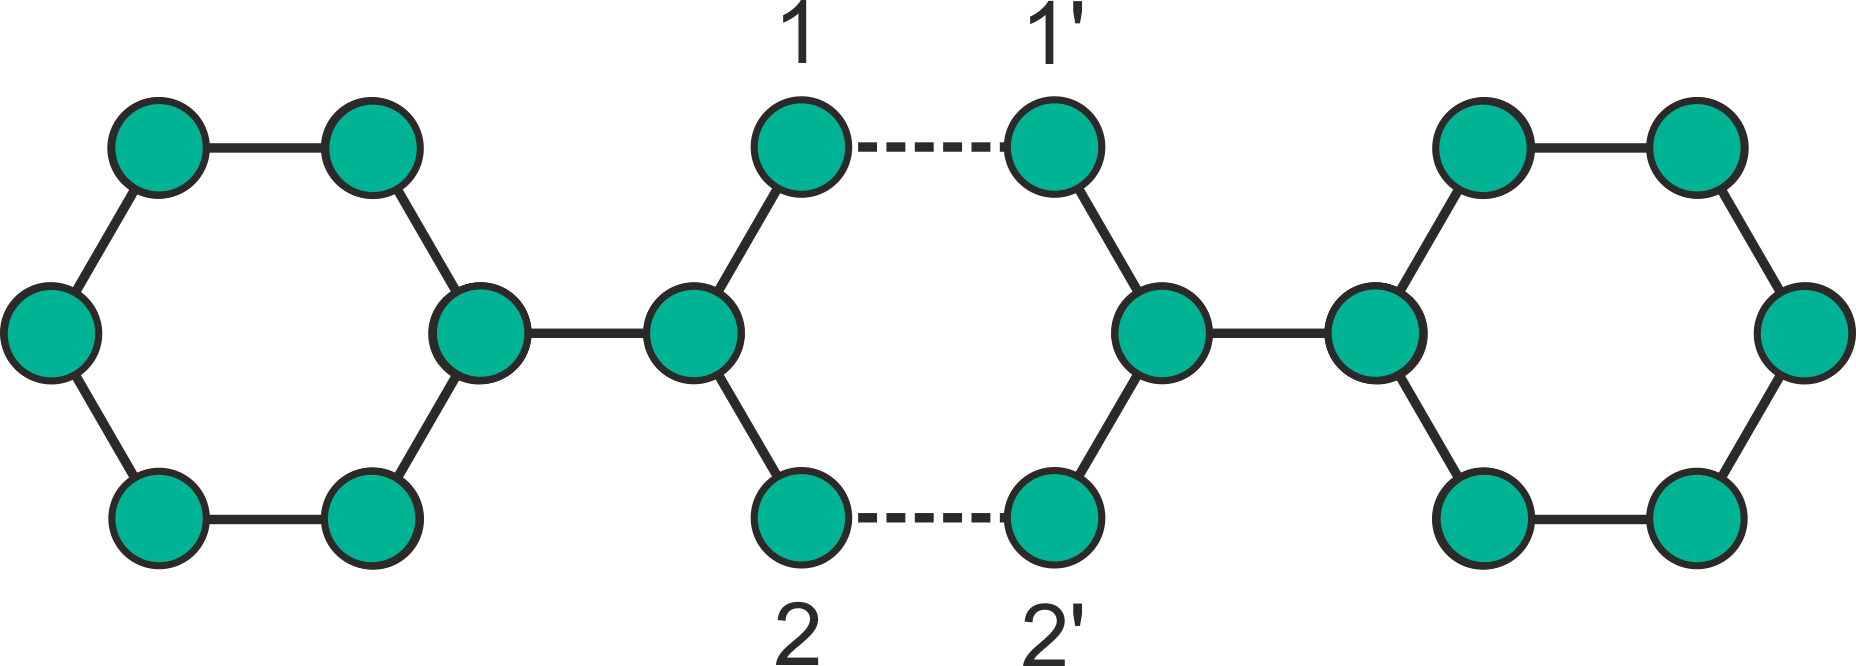
\includegraphics[width=40mm]{images/Fig_1_9_4_dec.png}
    \vspace{-5mm}
\end{wrapfigure}
4. Разделим $\pi$-систему п-терфенила на две одинаковых альтернантных системы, как показано на рисунке справа. Молекулярные орбитали неспаренного электрона: $\psi_{\textrm{НЭ}_1}=\frac{1}{\sqrt2}(\phi_1 -\phi_2)$ и $\psi_{\textrm{НЭ}_2}=\frac{1}{\sqrt2}(\phi_1' -\phi_2')$. Данные уровни вырождены, имеют энергию $E_{1,2}=\alpha$ и на них расположено 3 электрона (анион-радикал). Возмущение вида $\bra{\phi_1}V\ket{\phi_1’}=\bra{\phi_2}V\ket{\phi_2’}=\beta$ приводит к~поправкам к энергии $\Delta E_{1,2}=\pm \beta$. Тогда неспаренный электрон будет локализован на уровне, соответствующем поправке $\Delta E =-\beta$. Его правильная волновая функция имеет вид $\psi_{\textrm{НЭ}}=\frac{1}{\sqrt{2}}(\psi_{\textrm{НЭ}_1}-\psi_{\textrm{НЭ}_2})=\frac{1}{2}(\phi_1 -\phi_2-\phi_1' +\phi_2')$. Итого спиновая плотность равна $\rho_{1,\,2,\,1',\,2'}=1/4$.\par
5. Задача 5 контрольной работы 2 осеннего семестра 2023/2024 учебного года. Промежуточное состояние во всех случаях является одинаковой нечетной альтернантной системой. Используя МО неспаренного электрона можно посчитать $\pi$-заряд на центрах I, II, III: $q_{\text {I}}=26/51$; $q_{{\text {II}}}=1;$ $ q_{{\text {III}}}=50/51$. Тогда в~первом порядке теории возмущений изменение полной электронной энергии при введении –CH$_3$ группы в положение I, II или III: $\Delta E_{\text {I}}=26/51 \xi \beta$; $\Delta E_{{\text {II}}}=\xi \beta$; $\Delta E_{{\text {III}}}=50/51 \xi \beta$. Таким образом, повышение энергетического барьера меньше при замещении по положению I.\par
6. Вводим индуктивные заместители в $\pi$-систему бензола по теории возмущений: $\bra{\phi_1}{V}\ket{\phi_1}=\bra{\phi_2}{V}\ket{\phi_2}=\bra{\phi_4}{V}\ket{\phi_4}=\bra{\phi_5}{V}\ket{\phi_5}=\xi\beta$, где $ \xi=-0,1$. Поправки к энергиям уровней $E_{2,3}$ и $E_{4,5}$ равны $\Delta E_2 =\Delta E_4=\frac{1}{3}\xi\beta$, $\Delta E_3=\Delta E_5=\xi\beta$. Волновые функции не изменяются. В анион-радикале МО неспаренного электрона $\psi_4=\frac{1}{\sqrt{12}}(\phi_1+\phi_2-2\phi_3+\phi_4+\phi_5-2\phi_6)$, $\rho_{1,\,2,\,4,\,5}=1/12, \rho_{3,\,6}=1/3$. В~катион-радикале МО неспаренного электрона $\psi_3=\frac{1}{2}(\phi_1+\phi_2-\phi_4-\phi_5)$, $\rho_{1,\,2,\,4,\,5}=1/4$. Самый длинноволновый электрический дипольный переход имеет наименьшую энергию. В бензоле ($D_{6h}$) это переход из электронной конфигурации $(a_{2u})^2(e_{1g})^4$ терм $^1A_{1g}$ в конфигурацию $(a_{2u})^2(e_{1g})^3(e_{2u})^1$ термы $^{3,1}B_{1u}, {^{3,1}B_{2u}}, {^{3,1}E_{1u}}$. Переход $^1A_{1g}$ $\rightarrow$ ${^{1}E_{1u}}$ разрешен в $\sigma$ поляризации, Энергия перехода равна $\Delta E =-2\beta$. Cимметрия дурола $D_{2h}$. Наиболее длиноволновый переход имеет энергию $\Delta E \approx -1,933\beta$ и соответствует переходу с $\psi_3$ на $\psi_4$. Это переход из электронной конфигурации $(b_{1u})^2(b_{2g})^2(b_{3g})^2$ терм $^1{A_{g}}$ в конфигурацию $(b_{1u})^2(b_{2g})^2(b_{3g})^1(b_{1u})^1$ термы $^{3,1}{B_{2u}}$. Переход $^{1}{A_{g}}$ $\rightarrow$ $^{1}{B_{2u}}$ разрешен в $\sigma$ поляризации.\par
7. Для сравнения относительной устойчивости $\pi$-систем антрацена и фенантрена каждую из них удобно разделить на две одинаковые линейные альтернантные системы из 7 центров. Объединяя их назад по теории возмущений можно показать, что $\pi$-система антрацена является более устойчивой: $\Delta E_{\textrm{А}}=2\beta$; $\Delta E_{\textrm{Ф}}=3\beta / 2$.\par
8. Промежуточное состояние в данной реакции представляет собой $\pi$-систему аллильного радикала с дополнительным электроном ($S_N Ar$). В промежуточном состоянии $\pi$-заряд на центрах равен $q_{1,\,3}=3/2$, $q_{2}=1$. Используя выражение для изменения полной электронной энергии при введении заместителя $\Delta E^{(1)}=\sum_j q_j\Delta\alpha_j$, где $q_j$ – $\pi$-заряд на центре $j$, $\Delta\alpha_j$ – изменение кулоновского интеграла для $j$-того центра, можно показать, что нуклеофильное ароматическое замещение преимущественно реализуется в положение, расположенное ближе к –CF$_3$ группе, $\Delta E^{(1)}=0,35\beta$.\par
9. Задача 3 контрольной работы 2 осеннего семестра 2022/2023 учебного года.  Промежуточное состояние в обоих случаях является одинаковой нечетной альтернантной системой. Используя МО неспаренного электрона и $\pi$-заряд, в первом порядке теории возмущений определяем изменение полной электронной энергии при введении –CH$_3$ группы в положение 1 или 2: $\Delta E_1=3/2 \xi \beta$; $\Delta E_2=\xi \beta$. Таким образом, повышение энергетического барьера меньше при~замещении по положению 2.\par
10. Промежуточное состояние в данной реакции представляет собой альтернантную систему пентадиенильного радикала с 4 ($S_E Ar$) или 6 ($S_N Ar$) электронами. В случае нуклеофильного ароматического замещения $\pi$-заряд равен $q_{1,\,3,\,5}=4/3$, $q_{2,\,4}=1$. В случае электрофильного ароматического замещения $\pi$-заряд равен $q_{1,\,3,\,5}=2/3$, $q_{2,\,4}=1$. Используя теорию возмущений можно показать, что нуклеофильное замещение преимущественно протекает в положение 3, расположенное ближе к –CF$_3$ группе, $\Delta E^{(1)} = 0,3\beta$. Аналогично, электрофильное замещение преимущественно протекает в положение 2, расположенное ближе к –CH$_3$ группе, $\Delta E^{(1)}\approx 0,233\beta$.\par
\begin{wrapfigure}{r}{20mm} %this figure will be at the right
    \centering
    \vspace{-2ex}
    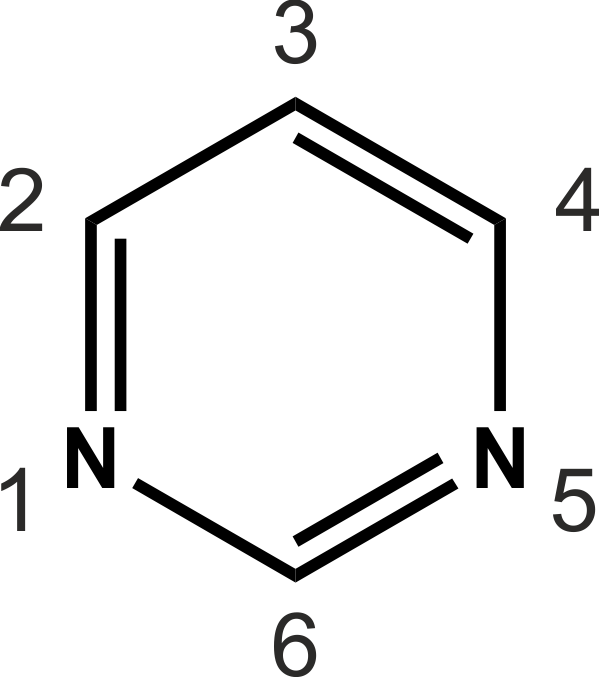
\includegraphics[width=12mm]{images/Fig_1_9_11_dec.png}
    \vspace{-5mm}
\end{wrapfigure}
11. Теоретический вопрос 2 дифференциального зачета осеннего семестра 2024/2025 учебного года. Изменяя кулоновский интеграл атома углерода на кулоновский интеграл атома азота по теории возмущений и нумеруя центры в пиримидине так, как показано на рисунке, можно получить МО неспаренного электрона: $\psi_{\text{НЭ}}=\frac{1}{\sqrt{12}}(2\phi_6+\phi_1+\phi_5-2\phi_3-\phi_2-\phi_4)$. Таким образом, спиновая плотность равна $\rho_{1,\,2,\,4,\,5}=1/12$; $\rho_{3,\,6}=4/12$.\par
\begin{wrapfigure}{r}{20mm} %this figure will be at the right
    \centering
    \vspace{-2ex}
    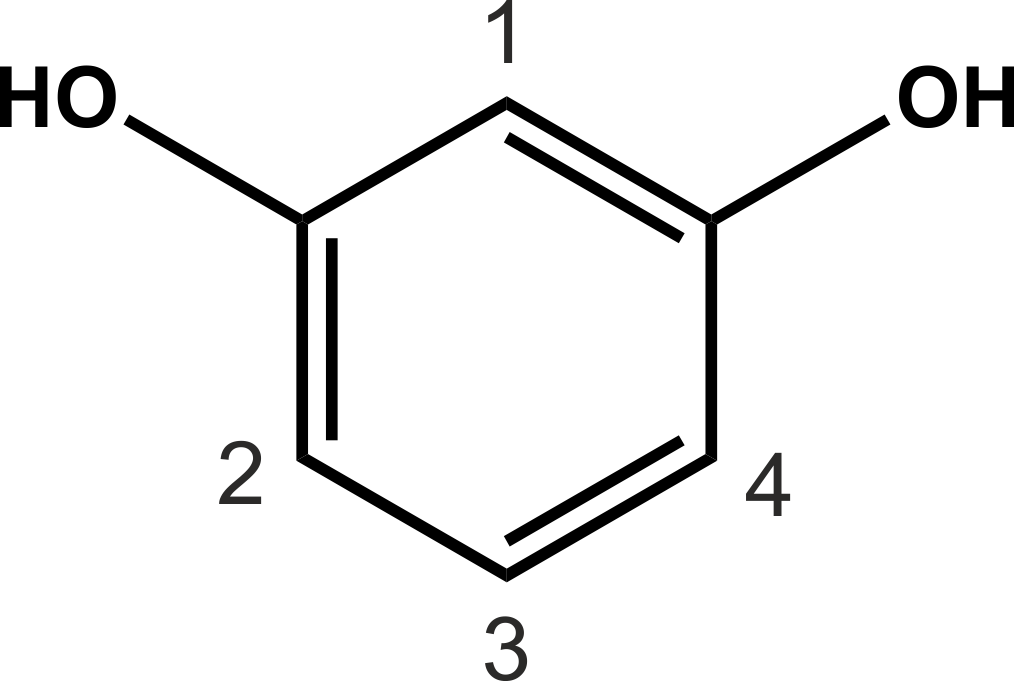
\includegraphics[width=19mm]{images/Fig_1_9_12_dec.png}
    \vspace{0mm}
\end{wrapfigure}
12. Группа –OH является +M мезомерным заместителем. Для определения преимущественного направления электрофильного замещения необходимо использовать второй порядок теории возмущений. Поправка к полной электронной энергии для случая электрофильного замещения при введении +M~заместителя может быть определена по выражению:
\begin{equation*}
\begin{aligned}
& \Delta E_{\Sigma}^{(2)}=2\sum_{\mu = m+1}^{n} \frac{C_{\mu r}^2 k^2}{h-\gamma_{\mu}} \beta, \hspace{58mm}
\end{aligned}
\end{equation*}
где $\alpha_{\text{O}}=\alpha_{\text{C}}+h\beta$, $\bra{\phi_{\text{O}}} V \ket{\phi_{\text{C}}}=k\beta$, $r$ – номер центра с –OH группой, $m$ – порядковый номер ВЗМО промежуточного состояния, $C_{\mu r}$ – коэффициент перед $r$-тым центром в $\mu$-той МО промежуточного состояния, $n$ – количество МО в~промежуточном состоянии. В данной задаче промежуточное состояние представляет собой $\pi$-систему пентадиенильного радикала с 4 электронами. Тогда, обозначая различные положения замещения как показано на рисунке, а также используя $h=1,2$ и $k=1,1$ получаются следующие поправки: (1) Положение 1: $2,032\beta$, (2) Положения 2, 4: $1,963\beta$, (3) Положение 3: $0,963\beta$. Таким образом, положение 1 является преимущественным направлением электрофильного замещения в~молекуле резорцина.\par
13. Необходимо сравнить полную электронную энергию $\pi$-систем промежуточных состояний, возникающих в процессе протекания данной реакции. Возможные варианты: (1) Замещение в положения 1, 2; Остается $\pi$-система бутадиена, $E_{\Sigma}\approx 4\alpha+4,47\beta$; (2) Замещение в положения 1, 3; Остается $\pi$-система аллильного радикала и изолированный центр, $E_{\Sigma}= 4\alpha+2\sqrt2\beta$; (3) Замещение в~положения 1, 4; Остаются две изолированных $\pi$-системы этилена, $E_{\Sigma}= 4\alpha+4\beta$. Полная электронная энергия минимальна в случае (1), который и является преимущественным направлением замещения. Полная электронная энергия промежуточного состояния для случая (2) отличается от случая (1) незначительно. Разница между данными вариантами может быть компенсирована характеристиками присоединяющихся радикальных частиц, например стерическим фактором. Наименее выгодным вариантом является вариант (2).\par
14. В бензоле ($D_{6h}$) самой высокой энергии соответствует запрещенный переход между конфигурациями $(a_{2u})^2(e_{1g})^4$ терм $^1{A_{1g}}$ и $(a_{2u})^1(e_{1g})^4(b_{2g})^1$ термы $^{3,1}B_{1u}$. Атомы дейтерия отличаются от атомов водорода кулоновским интегралом, который меняется на величину $\Delta \alpha =\alpha\frac{m_e}{2m_H} < 0$, см. задачу 1.2. Далее используем первый порядок теории возмущений: (1) $\bra{\phi_3}V\ket{\phi_3}=\bra{\phi_4}V\ket{\phi_4}=\Delta \alpha$ в случае 1,2-дидейтеробензола, (2)~$\bra{\phi_3}V\ket{\phi_3}=\bra{\phi_5}V\ket{\phi_5}=\Delta \alpha$ для 1,3-дидейтеробензола, (3)~$\bra{\phi_3}V\ket{\phi_3}=\bra{\phi_6}V\ket{\phi_6}=\Delta \alpha $ для 1,4-дидейтеробензола. Во всех случаях возмущение приводит к поправке $\Delta E_{1,\,6}^{(1)}= \Delta \alpha/3 $. Энергия перехода не~изменится и~различить изомеры не получится. При этом в отличие от бензола молекулы дидейтеробензола обладают более низкой симметрией, из-за чего для всех изомеров данный переход становится разрешенным.\par
15. Задача 2 дифференциального зачета осеннего семестра 2023/2024 учебного года. Направление преимущественного присоединения можно определить сравнивая индекс локализации для указанных трех случаев протекания реакции: $L=\sum_{\mu} n_{\mu}  \gamma_{\mu}^{\text{нач}} - \sum_{\mu} n_{\mu}  \gamma_{\mu}^{\text{кон}}$, где $n_{\mu}$ – количество электронов на $\mu$-ой МО, $\gamma_{\mu}$ – коэффициенты перед резонансными интегралами в энегрии $\mu$-ой МО: $\varepsilon_{\mu}=\alpha+\gamma_{\mu} \beta$. Поскольку начальное состояние во всех трех случаях одинаковое, то достаточно проанализировать второе слагаемое: $L'=\sum_{\mu} n_{\mu}  \gamma_{\mu}^{\text{кон}}$. Чем оно больше, тем вероятнее реакция. Центр I: конечное состояние – две $\pi$-системы этилена, $L'=4$; Центр II: конечное состояние – $\pi$-система аллильного радикала и изолированный центр, $L'=2,82$; Центр III: конечное состояние – $\pi$-система бутадиена, $L'=4,48$. Центр III является преимущественным направлением реакции присоединения атома водорода.\par
\newpage

%\usepackage[fit, breakall]{truncate}
%\phantomsection
\section[Спектроскопические методы исследования вещества]{\texorpdfstring{Электронное строение координационных соединений.\\Спектроскопические методы исследования вещества}{Электронное строение координационных соединений. Спектроскопические методы исследования вещества}}
%\addcontentsline{toc}{chapter}{2 Электронное строение координационных соединений. Спектроскопические методы исследования }
%\markboth{Электронное строение координационных соединений. Спектроскопические методы исследования}{Электронное строение координационных соединений. Спектроскопические методы исследования}
\subsection{Правила Вудворда-Хоффмана}
\begin{wrapfigure}{r}{30mm} %this figure will be at the right
    \centering
    \vspace{1.8mm}
    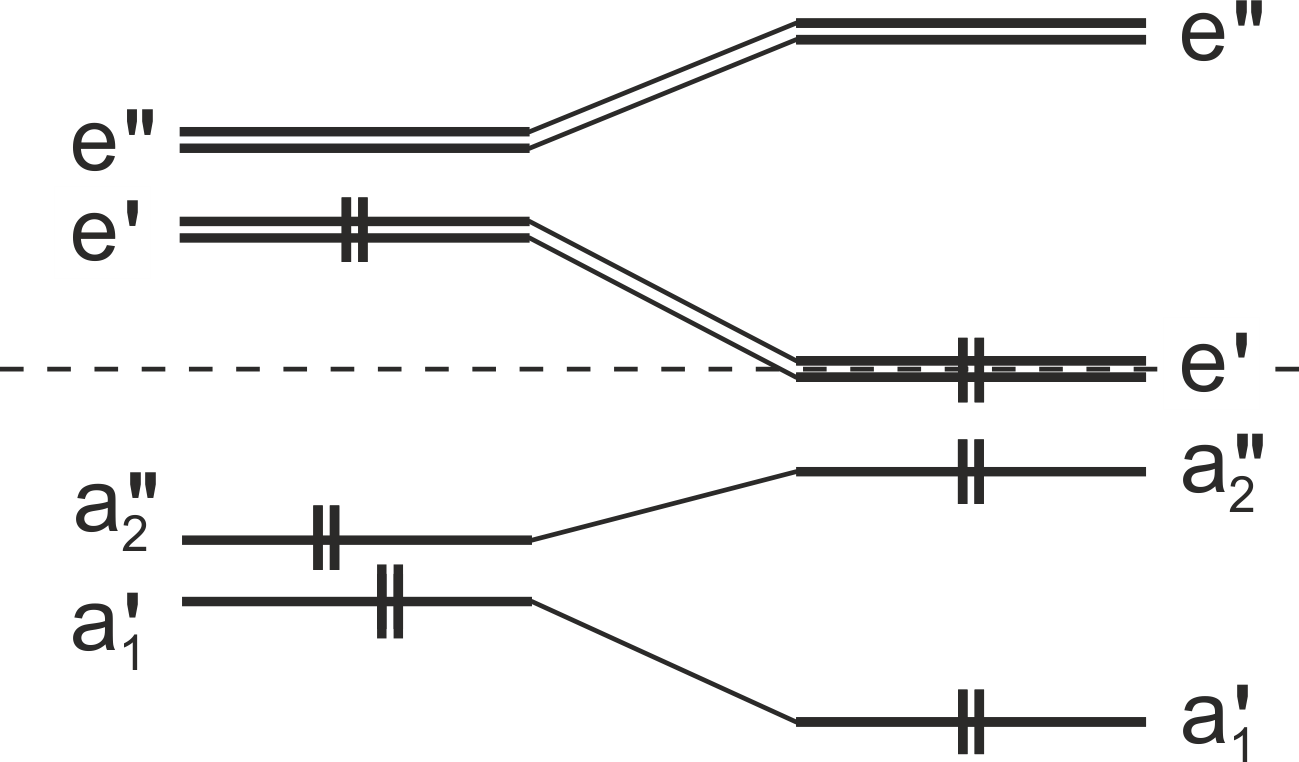
\includegraphics[width=30mm]{images/Fig_2_1_1_dec.png}
    \vspace{-5mm}
\end{wrapfigure}
1. Задача 3 контрольной работы 1 весеннего семестра 2021/2022 учебного года. Корреляционная диаграмма для группы симметрии $D_{3h}$ приведена на рисунке ниже.  Считая, что в реагентах молекулярные орбитали с симметрией $a'_1$ и $a''_2$, а также орбитали $e'$ и $e''$ имеют одинаковую энергию, изменение полной электронной энергии равно $2\beta$. Реакция разрешена термически.\par
\begin{wrapfigure}{r}{30mm} %this figure will be at the right
    \centering
    \vspace{-2.2mm}
    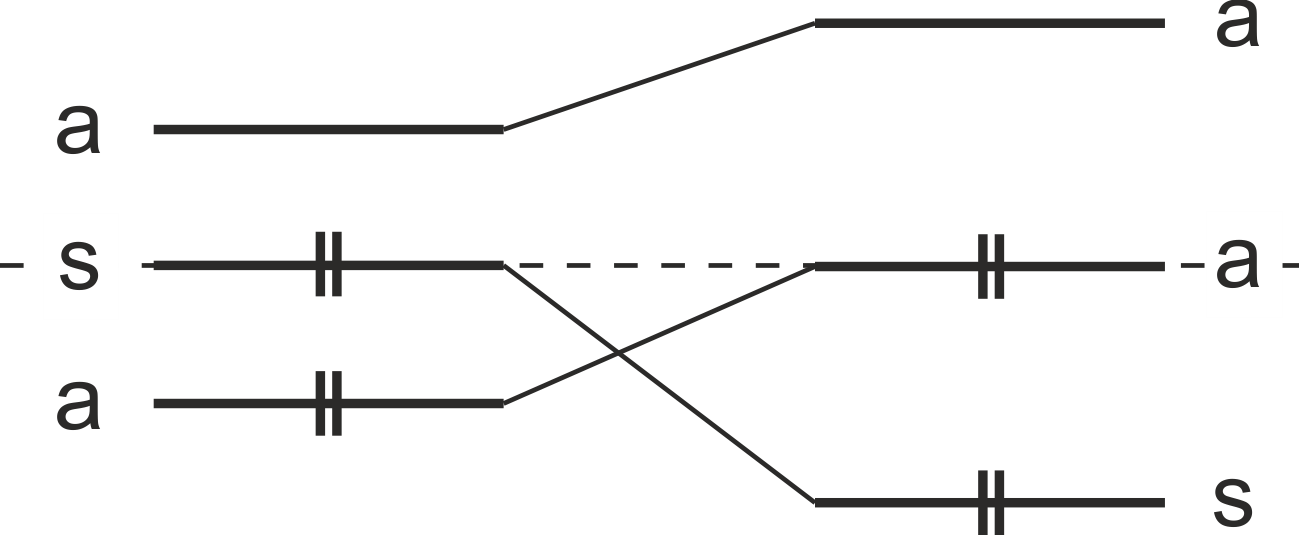
\includegraphics[width=30mm]{images/Fig_2_1_2_dec.png}
    \vspace{-5mm}
\end{wrapfigure}
2. Задача 1 контрольной работы 1 весеннего семестра 2023/2024 учебного года. Данная реакция термически протекает в конротаторном механизме, поэтому продуктом является цис-изомер, соответствующая корреляционная диаграмма приведена на рисунке.\par
3. В ходе реакции сохраняется группа симметрии $C_2$, при этом меняется направление единственной оси симметрии данной группы. Аналогично можно рассмотреть группу симметрии $D_2$. Реакция запрещена термически. Связывающая молекулярная орбиталь (МО) реагентов симметрии $b$ в базисе $2p_z$ атомных орбиталей становится разрыхляющей орбиталью продуктов, разрыхляющая МО реагентов симметрии $a$ становится связывающей орбиталью продуктов.\par
4. В $4\pi_s$ + $2\pi_s$ топологии реакция разрешена термически, есть ровно один $4n+2$ супра-компонент. В супра-/антара- топологии реакция запрещена термически, так как она соответствует, например, $2\pi_s$ + $2\pi_s$ + $2\pi_a$ компонентам. Корреляционная диаграмма для супра-/супра- топологии приведена на~рисунке. Для случая супра-/антара- топологии корреляционную диаграмму построить нельзя. В ходе реакции не сохраняется ни один элемент симметрии, см. рисунок.\par
\vspace{-\parskip}
\vspace{1mm}
\begin{figure}[h]
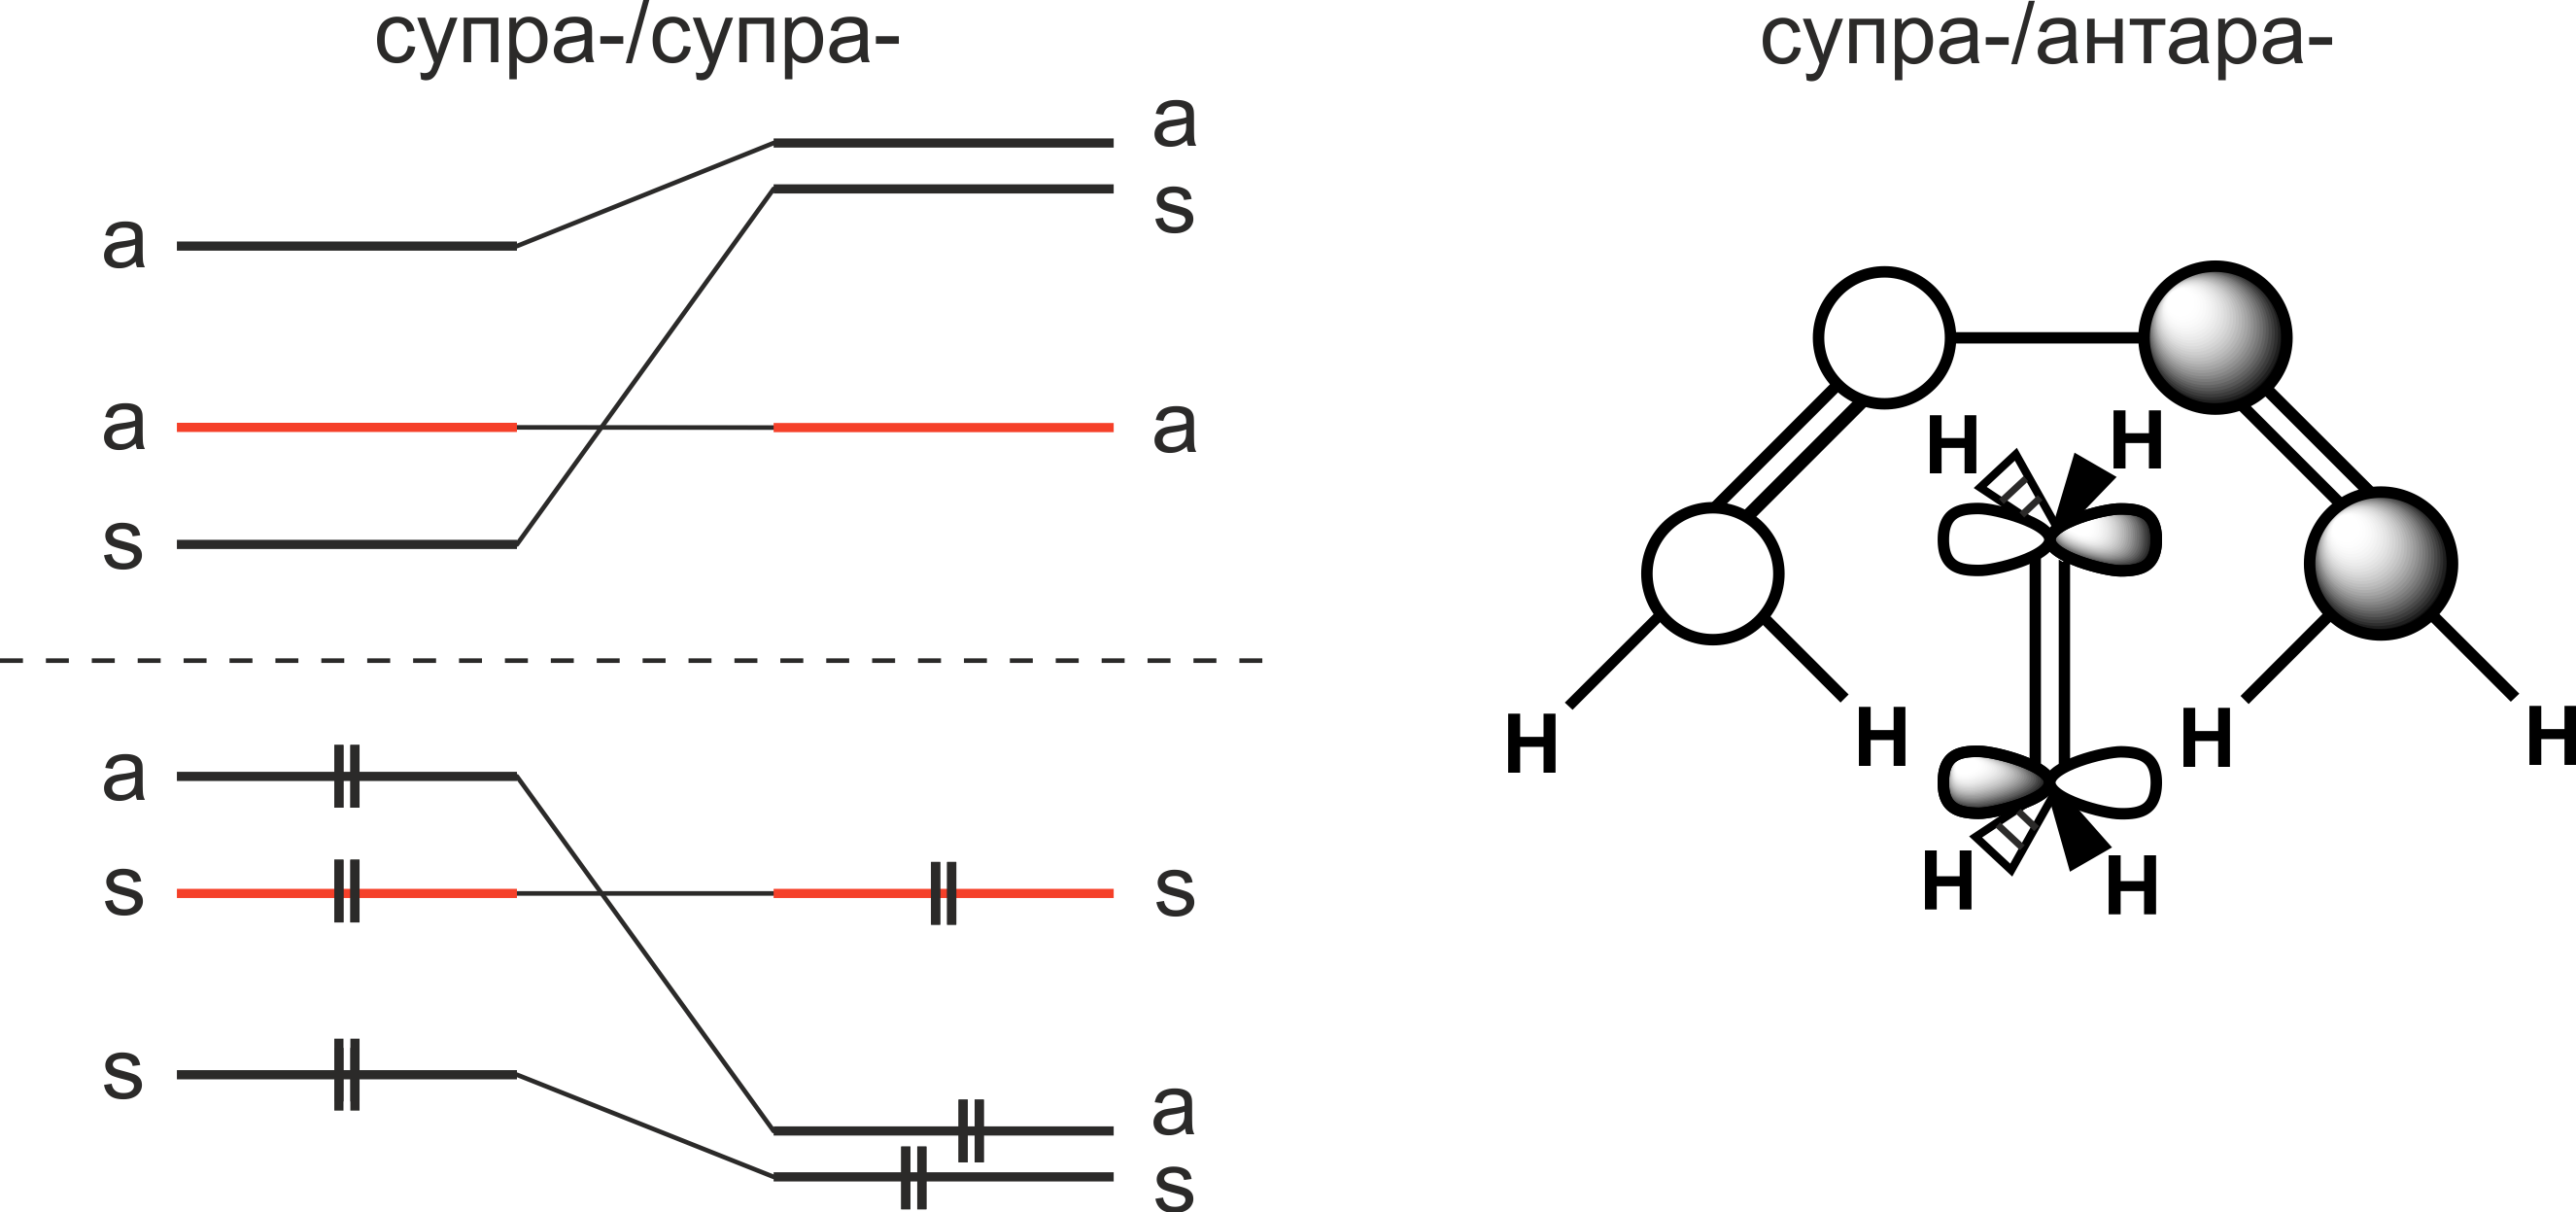
\includegraphics[width=6.5cm]{images/Fig_2_1_4_dec.png}
\centering
\end{figure}
\vspace{-\parskip}
\par
\begin{wrapfigure}{r}{30mm} %this figure will be at the right
    \centering
    \vspace{-0.7mm}
    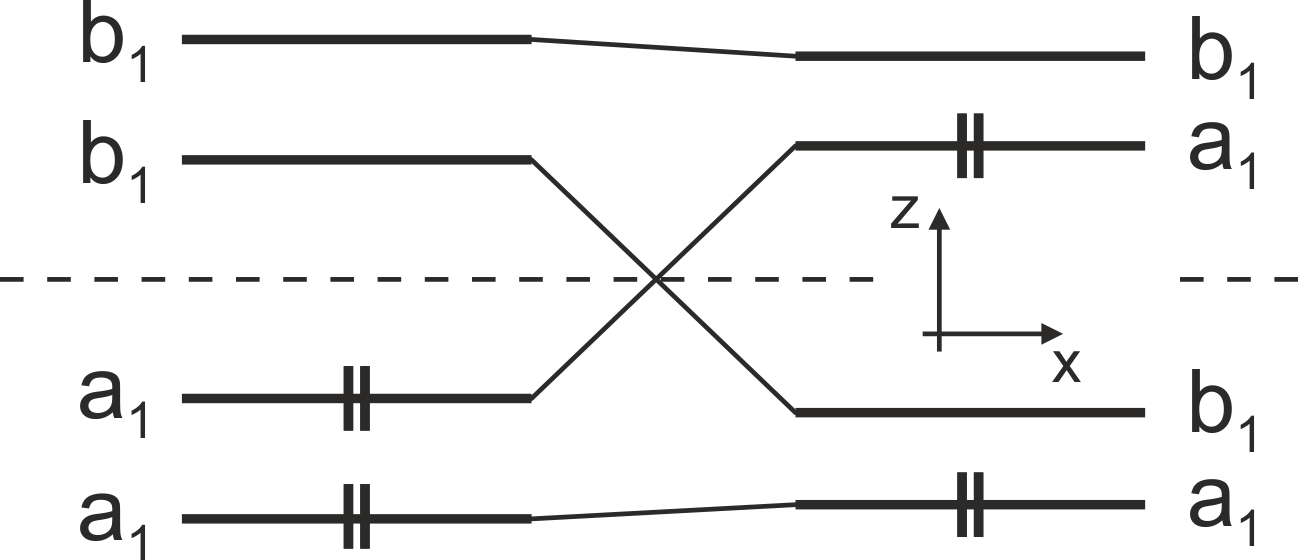
\includegraphics[width=30mm]{images/Fig_2_1_5_dec.png}
    \vspace{-9mm}
\end{wrapfigure}
5. В ходе всей реакции сохраняется группа симметрии  $C_{2v}$. Реакция протекает фотохимически. Корреляционная диаграмма приведена на рисунке.\par
%\vspace{-\parskip}
\begin{wrapfigure}{r}{30mm} %this figure will be at the right
    \centering
    \vspace{5.4mm}
    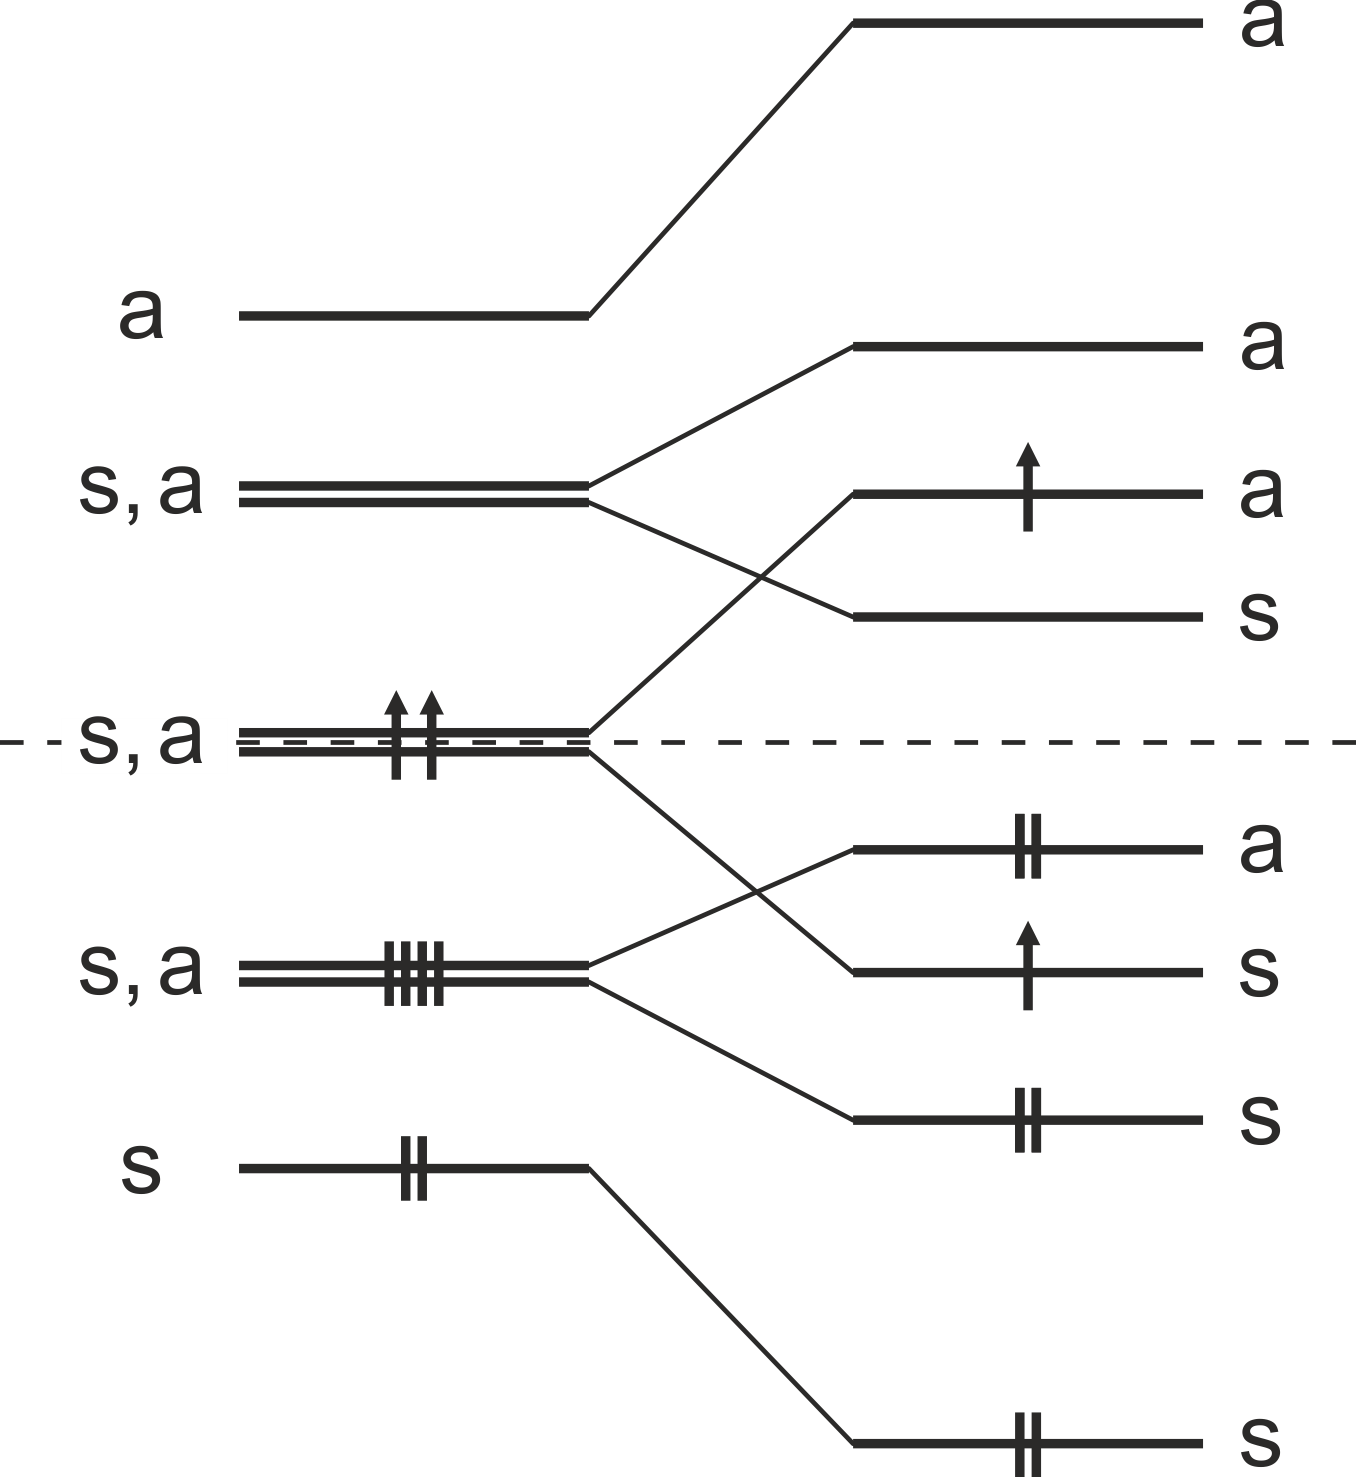
\includegraphics[width=30mm]{images/Fig_2_1_6_dec.png}
    \vspace{-5mm}
\end{wrapfigure}
6. Если считать, что циклооктатетраен плоский, то его основной терм триплетный по спину и реакция запрещена термически для дисротаторного механизма. Корреляционная диаграмма приведена на рисунке. Данный подход не совсем корректный. Если же учесть конформацию циклооктатетраена, необходимую для протекация реакции, то данная реакция в дисротаторном механизме соответствует трем $2\pi_s$ компонентам, то~есть она разрешена термически. В этом случае одна двойная связь выходит из сопряжения и~не участвует в~реакции. Реагент необходимо рассматривать как две линейные $\pi$-системы из 2 и 6 атомов, соответственно.\par
%\vspace{-\parskip}
\begin{wrapfigure}{r}{30mm} %this figure will be at the right
    \centering
    \vspace{-1mm}
    \includegraphics[width=30mm]{images/Fig_2_1_7_dec.png}
    \vspace{-5mm}
\end{wrapfigure}
7. В ходе всей реакции сохраняется группа симметрии $D_{2h}$. Корреляционная диаграмма для указанной в~условии системы координат и базиса $1s$ атомных орбиталей приведена на рисунке, реакция запрещена термически. Изменение полной электронной энергии равно $-2\beta$.\par
%\vspace{-\parskip}
8. Общая формулировка правил Вудворда-Хоффмана: перициклическая реакция термически разрешена если общее число $4n+2$ супраповерхностых и~$4n$~антараповерхностных компонент равно нечетному числу.  Более конкретно для~циклоприсоединения Дильса-Альдера, если $p+q=4n$, то реакция разрешена термически для супра-/антара- и антара-/супра- топологий, разрешена фотохимически для супра-/супра- и антара-/антара- топологий. Если $p+q=4n+2$, то~реакция разрешена термически для супра-/супра- и антара-/антара- топологий, разрешена фотохимически для супра-/антара- и антара-/супра- топологий. В~данном случае $p$ и $q$ равны количеству электронов в $\pi$-системах реагентов, а~$n$~– целое число.\par
%\vspace{-\parskip}
\begin{wrapfigure}{r}{30mm} %this figure will be at the right
    \centering
    \vspace{0mm}
    \includegraphics[width=30mm]{images/Fig_2_1_9_dec.png}
    \vspace{-5mm}
\end{wrapfigure}
9. В ходе всей реакции сохраняется группа симметрии $C_{2v}$. Корреляционная диаграмма приведена на рисунке. Реакция разрешена термически. Электрический дипольный переход в~H$_2$ возможен в конфигурацию $a_1^1b_1^1$, терм $^1B_1$. Фотохимически реакция также разрешена.\par
%\vspace{-\parskip}
10. Данная рекция может протекать как через промежуточное состояние в~конформации кресло, так и в конформации ванна. Рассмотрим для определенности только конформацию кресло. Как показано на рисунке, в этом случае реакция соответствует $2\pi_s$ + $2\pi_s$ + $2\sigma_s$ компонентам. Всего три $4n+2$ супра-компоненты, то есть реакция разрешена термически. Стереохимия продукта также приведена на рисунке. В случае конформации ванна данная реакция также разрешена термически.\par
\vspace{-\parskip}
\vspace{1mm}
\begin{figure}[h]
\includegraphics[width=6.5cm]{images/Fig_2_1_10_dec.png}
\centering
\end{figure}
\par
%\vspace{-\parskip}
\vspace{-\parskip}
\begin{wrapfigure}{r}{30mm} %this figure will be at the right
    \centering
    \vspace{4mm}
    \includegraphics[width=30mm]{images/Fig_2_1_11_dec.png}
    \vspace{-5mm}
\end{wrapfigure}
11. В ходе всей реакции сохраняется группа симметрии $C_s$ с единственной операцией симметриии $\sigma_{zx}$. Корреляционная диаграмма приведена на рисунке. Для простоты для атома азота учитываются только $2p$ атомные орбитали. Расположение молекулярных орбиталей по~энергии приведено качественно. Молекулярные орбитали молекулы водорода выделены красным цветом. Основное триплетное состояние реагентов коррелирует с возбужденным состоянием молекулы аммиака. Реакция запрещена термически.\par
12. Считаем, что при таком протекании реакции $3d$ атомные орбитали металла включены в систему молекулярных орбиталей. Их расщепление в поле двух этиленов для простоты не учитываем. В ходе всей реакции сохраняется группа симметрии $C_{2v}$. Корреляционная диаграмма приведена на рисунке. Реакция термически разрешена для электронных конфигураций $3d^2-3d^8$, без учета спиновой мультиплетности основного терма металла.\par
\vspace{-\parskip}
\vspace{1.5mm}
\begin{figure}[h]
\includegraphics[width=6.5cm]{images/Fig_2_1_12_dec.png}
\centering
\end{figure}
\par
13. Задача 2 контрольной работы 1 весеннего семестра 2024/2025 учебного года. Корреляционная диаграмма для супра-/супра- топологии приведена на~рисунке ниже.
\vspace{-\parskip}
\vspace{1.5mm}
\begin{figure}[h]
\includegraphics[width=8cm]{images/Fig_2_1_13_dec.png}
\centering
\end{figure}
\par
\vspace{-\parskip}
\newpage

\subsection{Теория кристаллического поля}
1. \\
2. 
\newpage

\subsection{Электронная спектроскопия}
1. \\
2. 
\newpage

\subsection{ИК и КР спектроскопии}
1. \\
2. 
\newpage

\subsection{Эффект Яна-Теллера}
1. \\
2. 
\newpage

\subsection{Вращательная спектроскопия и ее производные}
1. Предел канта равен $\frac{\text{d}}{\text{d}J}( \Delta E_R) = -\frac{1}{2}-\frac{B'}{B'-B}$, где $B'$ и $B$ – вращательные постоянные для колебательных состояний $\nu=1$ и $\nu=0$, соответственно. Подстановка межъядерного расстояния в эту формулу после округления до ближайшего целого числа дает 49.\par
2. $B=6,08114$ ГГц, $I=1,37\cdot10^{-45}$ кг$\cdot$м$^2$. Длины связей определяются из системы уравнений, составленной на основе моментов инерции изотопологов $^{16}\text{O}^{12}\text{C}^{32}\text{S}$ и~$^{16}\text{O}^{12}\text{C}^{34}\text{S}$, посчитанных с помощью приведенных в~условии данных.\par
3. \par
4. Группа симметрии $D_{4h}$, симметрический волчок. $A=B/2$.\par
5. X$-$X$-$Y линейная.\par
6. $J=2k$, $F=0$; $J=2k+1$, $F=1$, где $F$ – полный ядерный спин двух атомов водорода, $k$ – положительное целое число.\par
7. \par
8. \par
9. 25/64.\par
10. \par
11. Задача 2 контрольной работы 2 весеннего семестра 2024/2025 учебного года. $R=1,25\cdot10^{-10}$ м. Молекула HCl имеет приведенную массу, близкую к заданной в условии. \par
12. Задача 2 контрольной работы 2 весеннего семестра 2023/2024 учебного года. $B=3013,845$ МГц, $R=2,17\cdot10^{-10}$ м.\par
13. Задача 2 контрольной работы 2 весеннего семестра 2022/2023 учебного года. В обоих случаях чисто вращательный спектр будет представлять из себя набор эквидистантных линий, с расстоянием между линиями равным вращательной постоянной и относительной интенсивностью, определяемой населенностью вращательных уровней $N_J$. Населенность равна $(2J+1)\exp(-BJ(J+1)/kT)$ и~$(J+1)\exp(-BJ(J+1)/kT)$, соответственно, без учета и при учете описанного в~условии фактора. Анализ показывает, что максимум указанных величин $N_J$~достигается при $J_{max}\approx 2,65$ и $J_{max}\approx 2,41$. Таким образом, максимальной интенсивности будут обадать линии, соответствующие переходам с вращательных уровней $J=2$ и $J=3$.\par
\newpage

\subsection{ЭПР спектроскопия}
1. \\
2. 
\newpage

\subsection{Химический обмен в магнитном резонансе}
1. \\
2. 
\newpage

\subsection{ЯМР спектроскопия}
1. \\
2. 
\newpage


% Include the "notation" appendix from the BackMatter subfolder.
%\include{./BackMatter/notation}

% Include the "code" appendix from the BackMatter subfolder.
%\include{./BackMatter/code}

% Include the "glossary" appendix from the BackMatter subfolder.
%\include{./BackMatter/glossary}

% Include the "index" appendix from the BackMatter subfolder.
%\chapter{Index}

\blindtext

% Include the "references" appendix from the BackMatter subfolder.
%\bibliography{references.bib}
%\bibliographystyle{ieeetr}
%\nocite{*}
%\addcontentsline{toc}{chapter}{Список литературы}
%\thispagestyle{empty}


%%\bibliography{references.bib}
%\thispagestyle{empty}
%%\bibliographystyle{ieeetr}
\renewcommand*{\bibfont}{\footnotesize}
\nocite{*}
\printbibliography[heading=bibnumbered, title={Список литературы}]
%heading=bibnumbered, bibintoc
% End the document.
\end{document}
